% Options for packages loaded elsewhere
\PassOptionsToPackage{unicode}{hyperref}
\PassOptionsToPackage{hyphens}{url}
\PassOptionsToPackage{dvipsnames,svgnames,x11names}{xcolor}
\documentclass[
  10pt,
  a4paper]{article}
\usepackage{xcolor}
\usepackage[left=3cm,right=2cm,top=1cm,bottom=1cm,headheight=50pt,includeheadfoot]{geometry}
\usepackage{amsmath,amssymb}
\setcounter{secnumdepth}{5}
\usepackage{iftex}
\ifPDFTeX
  \usepackage[T1]{fontenc}
  \usepackage[utf8]{inputenc}
  \usepackage{textcomp} % provide euro and other symbols
\else % if luatex or xetex
  \usepackage{unicode-math} % this also loads fontspec
  \defaultfontfeatures{Scale=MatchLowercase}
  \defaultfontfeatures[\rmfamily]{Ligatures=TeX,Scale=1}
\fi
\usepackage{lmodern}
\ifPDFTeX\else
  % xetex/luatex font selection
\fi
% Use upquote if available, for straight quotes in verbatim environments
\IfFileExists{upquote.sty}{\usepackage{upquote}}{}
\IfFileExists{microtype.sty}{% use microtype if available
  \usepackage[]{microtype}
  \UseMicrotypeSet[protrusion]{basicmath} % disable protrusion for tt fonts
}{}
\makeatletter
\@ifundefined{KOMAClassName}{% if non-KOMA class
  \IfFileExists{parskip.sty}{%
    \usepackage{parskip}
  }{% else
    \setlength{\parindent}{0pt}
    \setlength{\parskip}{6pt plus 2pt minus 1pt}}
}{% if KOMA class
  \KOMAoptions{parskip=half}}
\makeatother
\usepackage{longtable,booktabs,array}
\usepackage{calc} % for calculating minipage widths
% Correct order of tables after \paragraph or \subparagraph
\usepackage{etoolbox}
\makeatletter
\patchcmd\longtable{\par}{\if@noskipsec\mbox{}\fi\par}{}{}
\makeatother
% Allow footnotes in longtable head/foot
\IfFileExists{footnotehyper.sty}{\usepackage{footnotehyper}}{\usepackage{footnote}}
\makesavenoteenv{longtable}
\usepackage{graphicx}
\makeatletter
\newsavebox\pandoc@box
\newcommand*\pandocbounded[1]{% scales image to fit in text height/width
  \sbox\pandoc@box{#1}%
  \Gscale@div\@tempa{\textheight}{\dimexpr\ht\pandoc@box+\dp\pandoc@box\relax}%
  \Gscale@div\@tempb{\linewidth}{\wd\pandoc@box}%
  \ifdim\@tempb\p@<\@tempa\p@\let\@tempa\@tempb\fi% select the smaller of both
  \ifdim\@tempa\p@<\p@\scalebox{\@tempa}{\usebox\pandoc@box}%
  \else\usebox{\pandoc@box}%
  \fi%
}
% Set default figure placement to htbp
\def\fps@figure{htbp}
\makeatother
% definitions for citeproc citations
\NewDocumentCommand\citeproctext{}{}
\NewDocumentCommand\citeproc{mm}{%
  \begingroup\def\citeproctext{#2}\cite{#1}\endgroup}
\makeatletter
 % allow citations to break across lines
 \let\@cite@ofmt\@firstofone
 % avoid brackets around text for \cite:
 \def\@biblabel#1{}
 \def\@cite#1#2{{#1\if@tempswa , #2\fi}}
\makeatother
\newlength{\cslhangindent}
\setlength{\cslhangindent}{1.5em}
\newlength{\csllabelwidth}
\setlength{\csllabelwidth}{3em}
\newenvironment{CSLReferences}[2] % #1 hanging-indent, #2 entry-spacing
 {\begin{list}{}{%
  \setlength{\itemindent}{0pt}
  \setlength{\leftmargin}{0pt}
  \setlength{\parsep}{0pt}
  % turn on hanging indent if param 1 is 1
  \ifodd #1
   \setlength{\leftmargin}{\cslhangindent}
   \setlength{\itemindent}{-1\cslhangindent}
  \fi
  % set entry spacing
  \setlength{\itemsep}{#2\baselineskip}}}
 {\end{list}}
\usepackage{calc}
\newcommand{\CSLBlock}[1]{\hfill\break\parbox[t]{\linewidth}{\strut\ignorespaces#1\strut}}
\newcommand{\CSLLeftMargin}[1]{\parbox[t]{\csllabelwidth}{\strut#1\strut}}
\newcommand{\CSLRightInline}[1]{\parbox[t]{\linewidth - \csllabelwidth}{\strut#1\strut}}
\newcommand{\CSLIndent}[1]{\hspace{\cslhangindent}#1}
\setlength{\emergencystretch}{3em} % prevent overfull lines
\providecommand{\tightlist}{%
  \setlength{\itemsep}{0pt}\setlength{\parskip}{0pt}}
\usepackage[brazil]{babel}
\usepackage{titling}
\usepackage[final]{pdfpages}
\usepackage{geometry}
\usepackage{subfig}
\usepackage{breqn}
\usepackage{booktabs}
%\usepackage{longtable}
\usepackage{textcomp}
\usepackage{graphics}
\usepackage{lastpage}
\usepackage{epigraph}
%\usepackage{csquotes}
\usepackage{dirtytalk}
\usepackage{lscape}
\setlength{\parindent}{1.25cm} % Default is 15pt.
\usepackage{indentfirst}
\usepackage{setspace}
\renewcommand{\baselinestretch}{1.5} 
%\usepackage{fontspec} % xelatex only
%%-----------------------------------------------------------------------
%\setmainfont{Times New Roman}
%\setsansfont{Arial}
%\setmonofont[Color={0019D4}]{Courier New}
%%-----------------------------------------------------------------------
%\usepackage{newtxtext} % Times New Roman
\usepackage{fontawesome5}
% with fontawesome5 you can use \faRProject to refer to R or use \Rlogo
\newcommand{\Rlogo}{\protect
\includegraphics[height=1.8ex,keepaspectratio]{Rlogo.png}}
\usepackage{fancyhdr}
\renewcommand{\footrulewidth}{0.4pt}
\pagestyle{fancy}
\fancyhf{}
\fancyhead[L]{
\includegraphics[width=15mm, height = 11mm]{logo.png}}
\fancyhead[CO,CE]{
%  
\includegraphics[width=15mm, height = 11mm]{logo.png}\\
\textbf{LAUDO DE AVALIAÇÃO}\\
\textbf{MÉTODO INVOLUTIVO}\\
%  Av. Afonso Delambert Neto, nº 103, Sala 7B, Lagoa da Conceição, Florianópolis/SC\\
%  (48)98426-1422
}
\fancyfoot[CO, CE]{Fazenda Rio Grande, Primavera do Leste, MT\\
Método Involutivo
}
\fancyfoot[R]{\thepage~de~\pageref{LastPage}}
\usepackage{booktabs}
\usepackage{longtable}
\usepackage{array}
\usepackage{multirow}
\usepackage{wrapfig}
\usepackage{float}
\usepackage{colortbl}
\usepackage{pdflscape}
\usepackage{tabu}
\usepackage{threeparttable}
\usepackage{threeparttablex}
\usepackage[normalem]{ulem}
\usepackage{makecell}
\usepackage{xcolor}
\usepackage{bookmark}
\IfFileExists{xurl.sty}{\usepackage{xurl}}{} % add URL line breaks if available
\urlstyle{same}
\hypersetup{
  pdftitle={Laudo de Avaliação},
  pdfauthor={Eng.~Luiz Fernando Palin Droubi; Eng.~Lutemberg de Araújo Florencio},
  colorlinks=true,
  linkcolor={red},
  filecolor={Maroon},
  citecolor={Blue},
  urlcolor={blue},
  pdfcreator={LaTeX via pandoc}}

\title{Laudo de Avaliação}
\usepackage{etoolbox}
\makeatletter
\providecommand{\subtitle}[1]{% add subtitle to \maketitle
  \apptocmd{\@title}{\par {\large #1 \par}}{}{}
}
\makeatother
\subtitle{Valor de uma gleba urbana}
\author{Eng.\textordmasculine~Luiz Fernando Palin
Droubi \and Eng.\textordmasculine~Lutemberg de Araújo Florencio}
\date{18/09/2025}

\begin{document}
\maketitle

\thispagestyle{fancy}

{
\hypersetup{linkcolor=}
\setcounter{tocdepth}{2}
\tableofcontents
}
\newpage

\section*{Resumo}\label{resumo}
\addcontentsline{toc}{section}{Resumo}

\begin{enumerate}
\def\labelenumi{\arabic{enumi}.}
\item
  \textbf{Nome Oficial}: Fazenda Rio Grande
\item
  \textbf{Endereço do Imóvel}: Rodovia BR 070 Km 272 a Esquerda,
  Primavera do Leste, MT.
\item
  \textbf{Tipo do Imóvel}: Terreno (gleba)
\item
  \textbf{Solicitante}: Protásio Vargas Neto.
\item
  \textbf{Proprietário}: Antônio Agilberto Vargas e Elizabete Mascarello
\item
  \textbf{Objetivo}: Determinar o valor de mercado.
\item
  \textbf{Finalidade}: Alienação da gleba.
\item
  \textbf{Resumo dos Valores de Avaliação}:
\end{enumerate}

\begin{center}
\textbf{Estimativa de Valor Central:}
\end{center}

\[V_{gleba} = \text{R\$ }161.000.000,00 \]

\begin{center}
\vspace*{2\baselineskip}
\textbf{Intervalo de Valores Prováveis:}
\end{center}

\[[148.400.000,00; \;174.150.000,00]\]

\begin{enumerate}
\def\labelenumi{\arabic{enumi}.}
\setcounter{enumi}{8}
\item
  \textbf{Especificação}: Grau II de fundamentação.
\item
  \textbf{Data de Referência}: set/2025
\item
  \textbf{Responsáveis técnicos}: \theauthor
\end{enumerate}

\newpage

\section{Introdução}\label{introduuxe7uxe3o}

O presente Laudo foi elaborado seguindo os preceitos NBR-14.653 -- Norma
Brasileira para Avaliação de Bens -\/-- Partes 1 e 2 -- da Associação
Brasileira de Normas Técnicas (\citeproc{ref-NBR1465302}{ABNT, 2011},
\citeproc{ref-NBR1465301}{2019}).

\subsection{Objeto}\label{objeto}

O imóvel objeto da avaliação é uma gleba constituída de duas matrículas
independentes, situados em perímetro urbano, mais especificamente
localizado na Zona Urbana Intermediária, segundo plano diretor de
Primavera do Leste/MT, conforme mapa apresentado no
\hyperref[anexo-viii]{ANEXO VIII}. O imóvel apresenta atualmente uso
rural (cultivo de soja e milho), contando com área de 315,97 ha,
(3.159.722 \(m^2\)), localizado à margem esquerda da Rodovia BR-070, km
272.

\section{Objetivo e Finalidade}\label{objetivo-e-finalidade}

\begin{itemize}
\tightlist
\item
  \textbf{Objetivo}
\end{itemize}

Determinar o valor de mercado.

\begin{itemize}
\tightlist
\item
  \textbf{Finalidade}
\end{itemize}

Alienação da gleba.

\section{Metodologia Adotada}\label{metodologia-adotada}

Método Involutivo.

\subsection{Escolha com justificativa:}\label{escolha-com-justificativa}

A NBR 14.653-1/2019(\citeproc{ref-NBR1465301}{ABNT, 2019}), conceitua o
Método Involutivo em seu item 7.2.2, \emph{in verbis}:

\epigraph{Método Involutivo: Identifica o valor do bem, alicerçado no seu 
aproveitamento eficiente, baseado em modelo de estudo de viabilidade 
técnico-econômica, mediante hipotético empreendimento compatível com as 
características do bem e com as condições do mercado no qual está inserido, 
considerando-se cenários viáveis para execução e comercialização do produto. O
método involutivo pode identificar o valor de mercado. No caso de utilização de
premissas especiais, o resultado é um valor especial.}{NBR 14.653-01 \\ 7.7.2}

Utilizou-se o Método Involutivo devido a inexistência de imóveis em
quantidade necessária e suficientemente semelhantes ao avaliando para
adoção do Método Comparativo Direto de Dados de Mercado. Tal limitação
justifica o emprego do método involutivo.

\section{Documentação utilizada}\label{documentauxe7uxe3o-utilizada}

Consigna-se que o presente trabalho avaliatório considerou como
documentação de referência:

\begin{itemize}
\tightlist
\item
  Cópia (digitalizada) da Certidão de inteiro teor, datada de
  04/03/2024, referente à Matrícula nº 45.556, emitida pelo Registo de
  Imóveis da Circunscrição da Comarca de Primavera do Leste (MT);
\item
  Cópia (digitalizada) da Certidão de inteiro teor, datada de
  27/05/2025, referente à Matrícula nº 34.497, emitida pelo Registo de
  Imóveis da Circunscrição da Comarca de Primavera do Leste (MT);
\item
  Arquivo KML (\emph{Keyhole Markup Language}), disponibilizado pelo
  solicitante, com a identificação da poligonal dos imóveis constantes
  nas matrículas nº 45.556 e nº 34.497, com áreas de 176,22 ha e 139,76
  ha, respectivamente.
\item
  Certificados de Cadastro de Imóvel Rural (CCIR) do INCRA, Emissão
  Exercício 2019
\end{itemize}

A documentação acima referida (exceto arquivo KML) pode ser vista no
\hyperref[anexo-ix]{ANEXO IX}.

\section{Pressupostos, ressalvas e fatores
limitantes}\label{pressupostos-ressalvas-e-fatores-limitantes}

O avaliador considera que os elementos a ele fornecidos são legítimos e
que as informações prestadas por terceiros foram dadas de boa fé,
merecendo, portanto, todo o crédito.

Foram admitidas como verdadeiras as informações constantes nos
documentos e projetos/plantas de engenharia fornecidos pelo solicitante,
tais como áreas, dimensões, confrontantes, compartimentos, tipologias
entre outras características inerentes ao avaliando. Referidas
informações não foram objeto de validação minuciosa pelo avaliador. Ao
contrário, por ocasião da vistoria, foram observados apenas aspectos
gerais, com base em inspeção visual, sem a utilização de instrumentos de
precisão. O avaliador não assume responsabilidade sobre matéria legal ou
de engenharia, fornecidos pelo interessado. Caso ocorram alterações ou
não se confirmem as referidas informações, o(s) valor(es) apresentados
deverão ser revistos pelo avaliador.

O imóvel foi avaliado na suposição de que esteja livre e desembaraçado
de quaisquer ônus, encargos ou gravames de qualquer natureza que possam
afetar o seu valor, pressupondo que as áreas e características
informadas, bem como seus respectivos títulos estejam corretos e que a
documentação enviada para consulta seja a vigente.

Consigna-se que o presente trabalho avaliatório considerou como premissa
da avaliação que o imóvel avaliando, denominado ao longo deste laudo de
``Fazenda Rio Grande'', é constituído por dois terrenos com matrículas
independentes (nº 45.556 e nº 34.497), porém contíguos, perfazendo uma
área total de 315,97 ha, conforme arquivo KML (\emph{Keyhole Markup
Language}) disponibilizado pelo solicitante. Registra-se que a referida
área (315,97 ha) diverge do somatório das áreas informadas nas Certidões
e nos Certificados de Cadastro de Imóvel Rural (CCIR) dos supracitados
imóveis (matrículas nº 45.556 e nº 34.497). Contudo, conforme
previamente acordado com o solicitante, o pressuposto desta avaliação é
considerar a área total informada no arquivo KML, ou seja, 315,97 ha.

O signatário não assume responsabilidade sobre matéria legal ou de
engenharia, fornecidos pelo interessado.

Não foram efetuadas quaisquer análises jurídicas da documentação do
imóvel, por não se integrarem com o escopo desta avaliação, não tendo
sido efetuadas medições de campo para a finalidade desta avaliação. Não
foram consultados os órgãos públicos de âmbito Municipal, Estadual ou
Federal, quanto à situação legal do imóvel perante os mesmos.

Nenhum estudo de impacto ambiental foi solicitado ou realizado. Para
efeito de avaliação, partiu-se do pressuposto da inexistência de passivo
ambiental sobre o bem, sendo assumida a total obediência às leis e
regulamentos ambientais no âmbito federal, estadual e municipal, a menos
que declarado em contrário.

A respeito das áreas verdes, constatou-se que os imóveis possuem área
menor do que 4 módulos fiscais. Nesta situação, a Reserva Legal do
imóvel é constituída da vegetação nativa presente na data de 22/07/2008,
conforme código florestal vigente (ver
\href{https://www.embrapa.br/codigo-florestal/area-de-reserva-legal-arl}{link}).
Conforme consultas à especialistas em perícias ambientais,
considerou-se, de comum acordo com o Contratante, que as áreas
identificadas como de vegetação nativa não tiveram seu uso modificado no
projeto hipotético. Considerou-se ainda, também de comum acordo com o
Contratante, que a alteração de uso do imóvel (rural para industrial)
será feita mantendo-se a área de reserva legal existente, conforme
orientação de perito ambiental consultado.

Esta avaliação é independente e livre de quaisquer vantagens ou
envolvimento das pessoas que realizaram os serviços.

Os valores encontrados estão fixados em moeda corrente Real (R\$) e para
a data base de seus cálculos.

Registra-se que a estimativa do valor de mercado do lote paradigma --
integrante do projeto hipotético do loteamento industrial -- com a
finalidade de subsidiar a aplicação do Método Involutivo para determinar
o valor da gleba objeto da presente avaliação, consta no
\hyperref[anexo-i]{ANEXO I}.

As avaliações foram feitas de acordo com as normas brasileiras de
avaliação NBR 14653-1 --
\say{Avaliação de bens – Parte 1: Procedimentos Gerais}
(\citeproc{ref-NBR1465301}{ABNT, 2019}) e NBR 14653-2 --
\say{Avaliação de bens – Parte 2: Imóveis urbanos}
(\citeproc{ref-NBR1465302}{ABNT, 2011}).

\section{Localização do Imóvel}\label{localizauxe7uxe3o-do-imuxf3vel}

Trata-se de uma gleba, denominada de \say{Fazenda Rio Grande},
localizada às margens da Rodovia BR-070, Km 272, na cidade de Primavera
do Leste (MT), constituída por dois terrenos com matrículas
independentes, com números 34.497 e 45.556 do Livro n.º 2 do Registro de
Imóveis da Comarca de Primavera do Leste - MT, porém contíguos,
perfazendo uma área total de 315,97 ha (ver
\hyperref[pressupostos-ressalvas-e-fatores-limitantes]{Pressupostos,
ressalvas e fatores limitantes}).

A título de referência, registra-se que o imóvel avaliando está situado
na vizinhança do distrito industrial José de Alencar, em zona de
expansão urbana, lado esquerdo da rodovia BR-070, distando cerca de 3,5
km do conglomerado urbano de Primavera do Leste.

As coordenadas geográficas registradas na porteira de acesso do imóvel
(BR-070): -15.542142, -54.238286; Datum: WGS 84

OBS.: Os limites e confrontantes do imóvel avaliando podem ser
visualizados no arquivo KML (\emph{Keyhole Markup Language})
disponibilizado pelo solicitante.

Registra-se que o avaliando apresenta formato irregular, topografia com
leve aclive para os fundos e solo aparentemente seco.

A Figura \ref{fig:Perimetro} mostra a localização do imóvel avaliando
sobre uma imagem de fundo de satélite obtida de \emph{Stadia Maps}.

\begin{figure}[H]

{\centering \includegraphics[width=0.9\linewidth]{images/Perimetro-1} 

}

\caption{Localização do imóvel avaliando.}\label{fig:Perimetro}
\end{figure}

\subsection{Descrição da região, entorno e
acessos}\label{descriuxe7uxe3o-da-regiuxe3o-entorno-e-acessos}

O avaliando está situado em Primavera do Leste (MT), município
localizado a aproximadamente 239 km da capital, Cuiabá. Este possui uma
área de 5.247,897 \(km^2\), com população total estimada em 68.523
habitantes, o que corresponde a uma densidade demográfica de
aproximadamente 13,06 habitantes/\(km^2\) (IBGE, 2022).

As principais atividades econômicas do município estão ligadas ao
agronegócio, destacando-se a produção de soja, milho, algodão e feijão,
além da produção de arroz e sorgo. Outras cadeias produtivas relevantes
incluem a bovinocultura de corte e leite, bem como a avicultura e a
suinocultura. O município também possui crescente atividade industrial,
especialmente nas áreas de beneficiamento de grãos, produção de insumos
agrícolas e apoio logístico ao setor agroindustrial.

Primavera do Leste vem apresentando constante crescimento econômico e
demográfico nas últimas décadas, impulsionado principalmente pelo avanço
do agronegócio e pela consequente atração de empresas e indústrias do
setor. O desenvolvimento urbano tem acompanhado esta expansão,
resultando em melhorias na infraestrutura local e maior diversificação
da economia municipal.

\section{Vistoria}\label{vistoria}

A vistoria foi realizada em 09/07/2025. As Figuras abaixo ilustram a
situação da propriedade na data da vistoria.

As Figuras \ref{fig:Porteira1} e \ref{fig:Porteira2} mostram que a
propriedade o acesso principal da propriedade, pela BR-070. A Figura
\ref{fig:Sede} mostra a pequena sede existente, com ligação de energia e
água de poço. A Figura \ref{fig:Barracao} mostra uma benfeitoria da
propriedade (barracão). A Figura \ref{fig:Carreadores} ilustra como são
os carreadores internos da propriedade. Por fim, a Figura
\ref{fig:Vegetacao} mostra que há vegetação esparsa em alguns pontos da
propriedade e, aos fundos, uma vegetação mais densa, mais importante,
por fazer parte de uma área de provável proteção permanente (APP),
denominada Furnas.

\begin{figure}[H]

{\centering 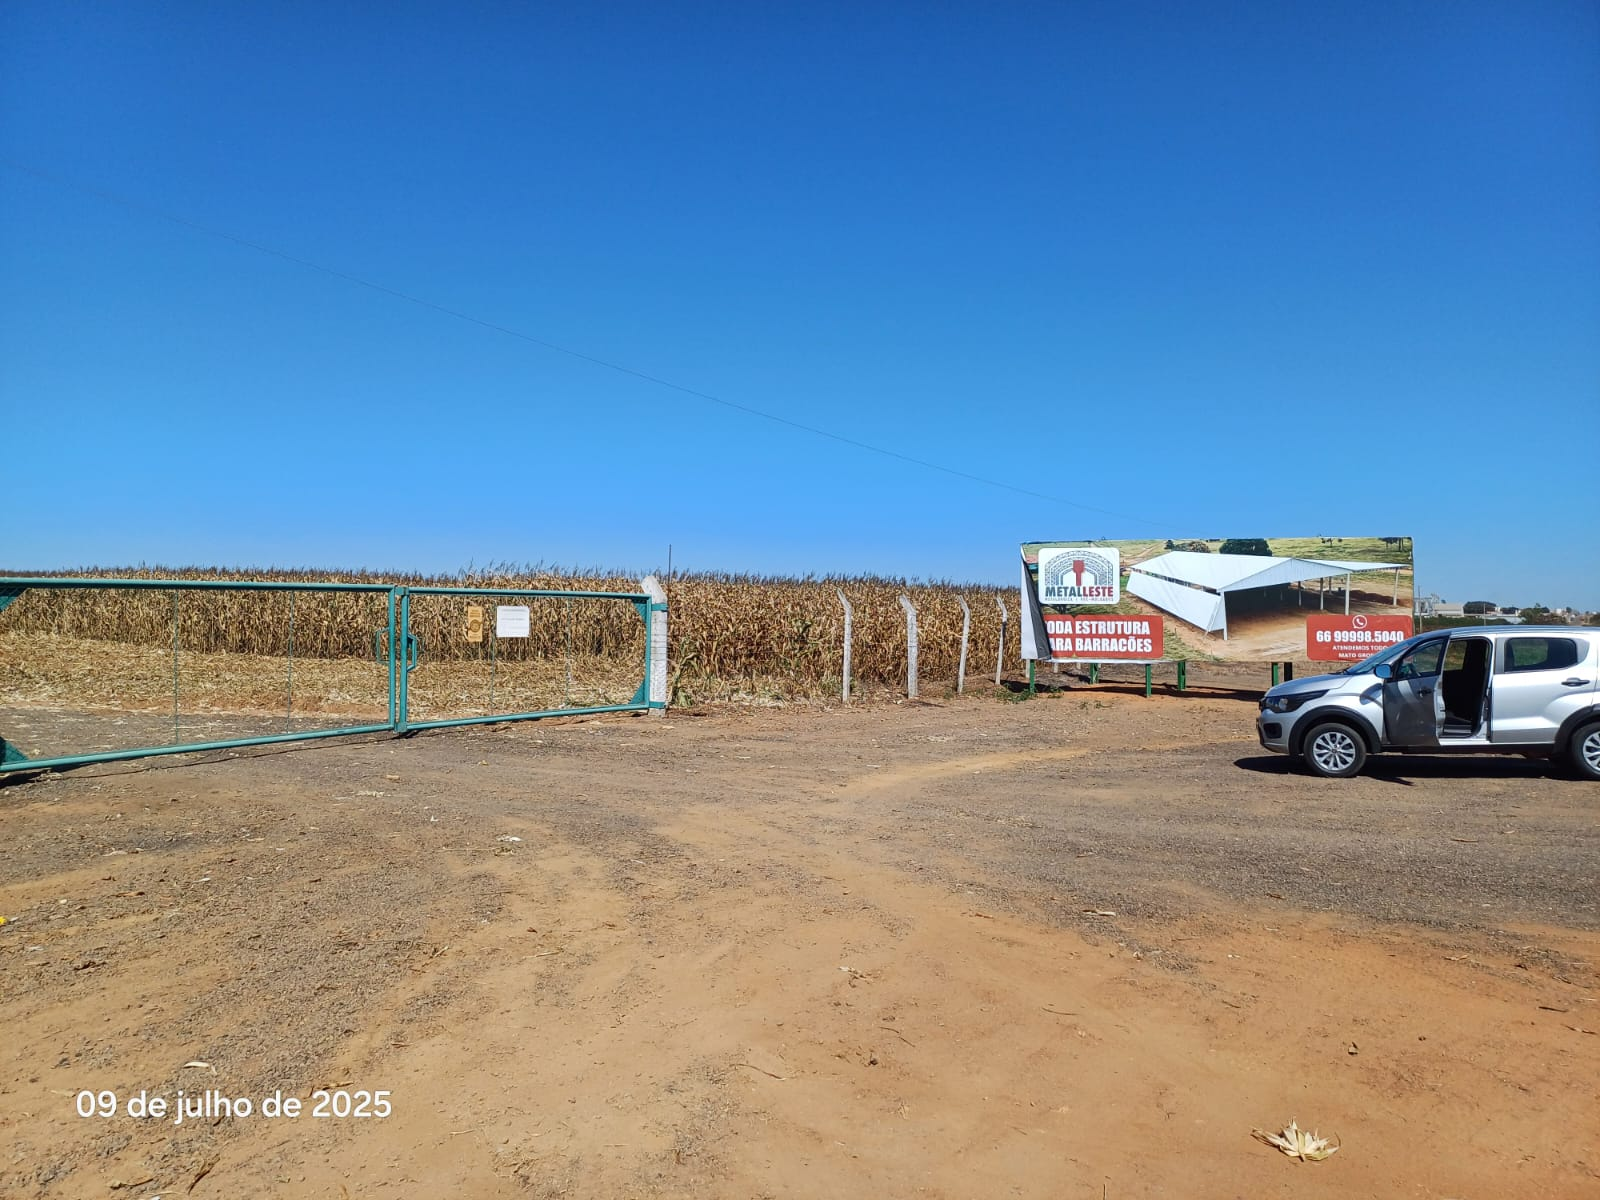
\includegraphics[width=0.49\linewidth]{./refs/Fotos/39} 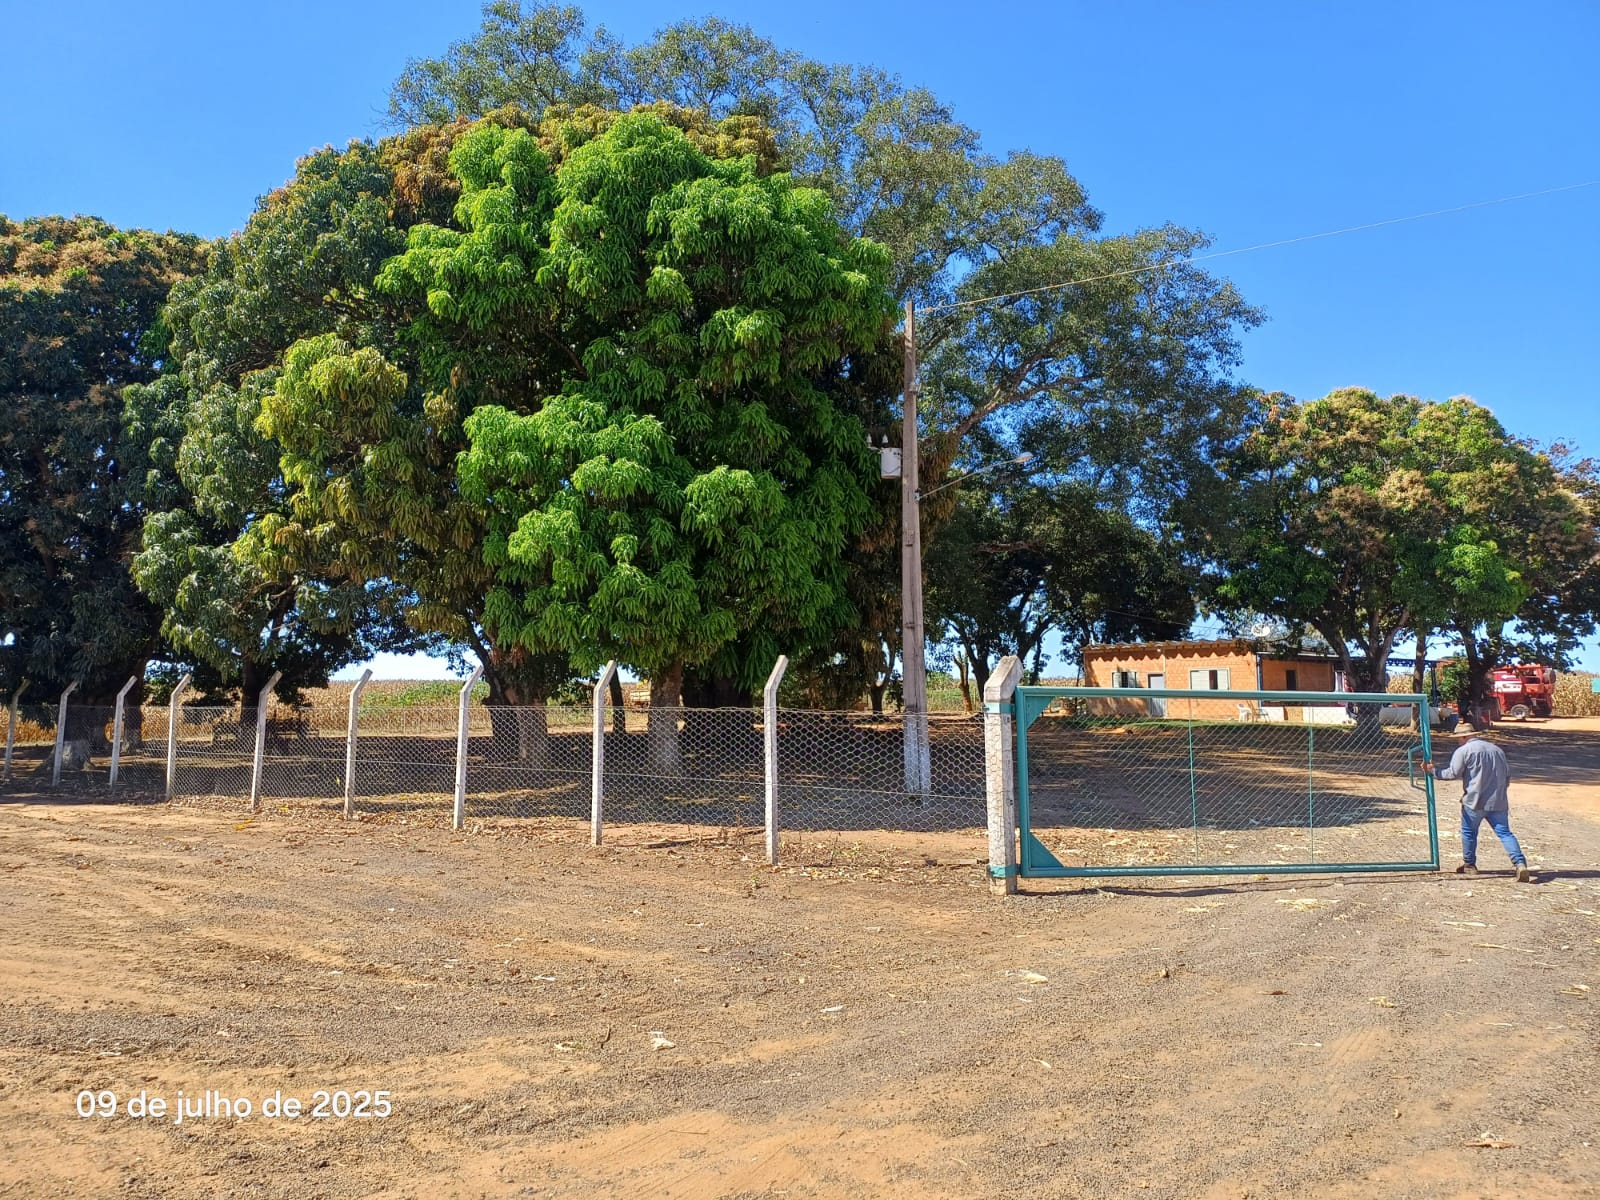
\includegraphics[width=0.49\linewidth]{./refs/Fotos/37} 

}

\caption{Porteira de acesso da propriedade}\label{fig:Porteira1}
\end{figure}

\begin{figure}[H]

{\centering 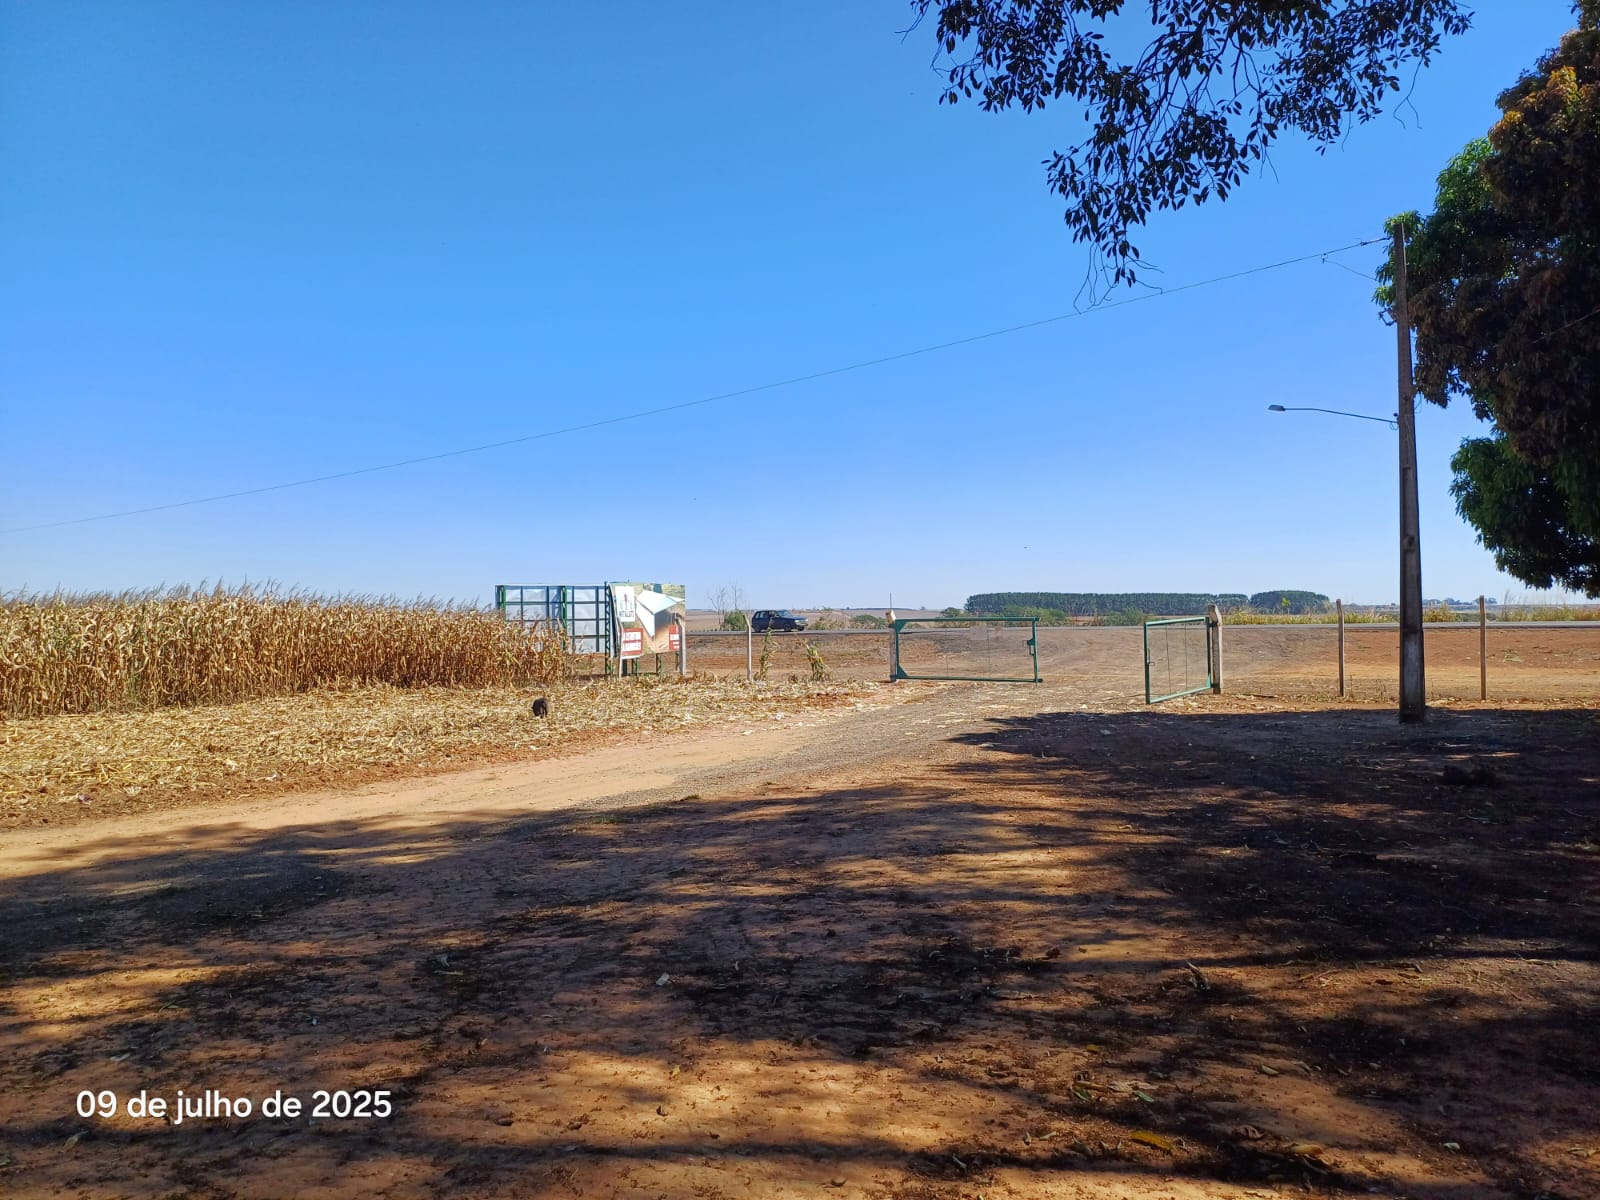
\includegraphics[width=0.7\linewidth]{./refs/Fotos/34} 

}

\caption{Porteira de acesso da propriedade. Vista Interna.}\label{fig:Porteira2}
\end{figure}

\begin{figure}[H]

{\centering 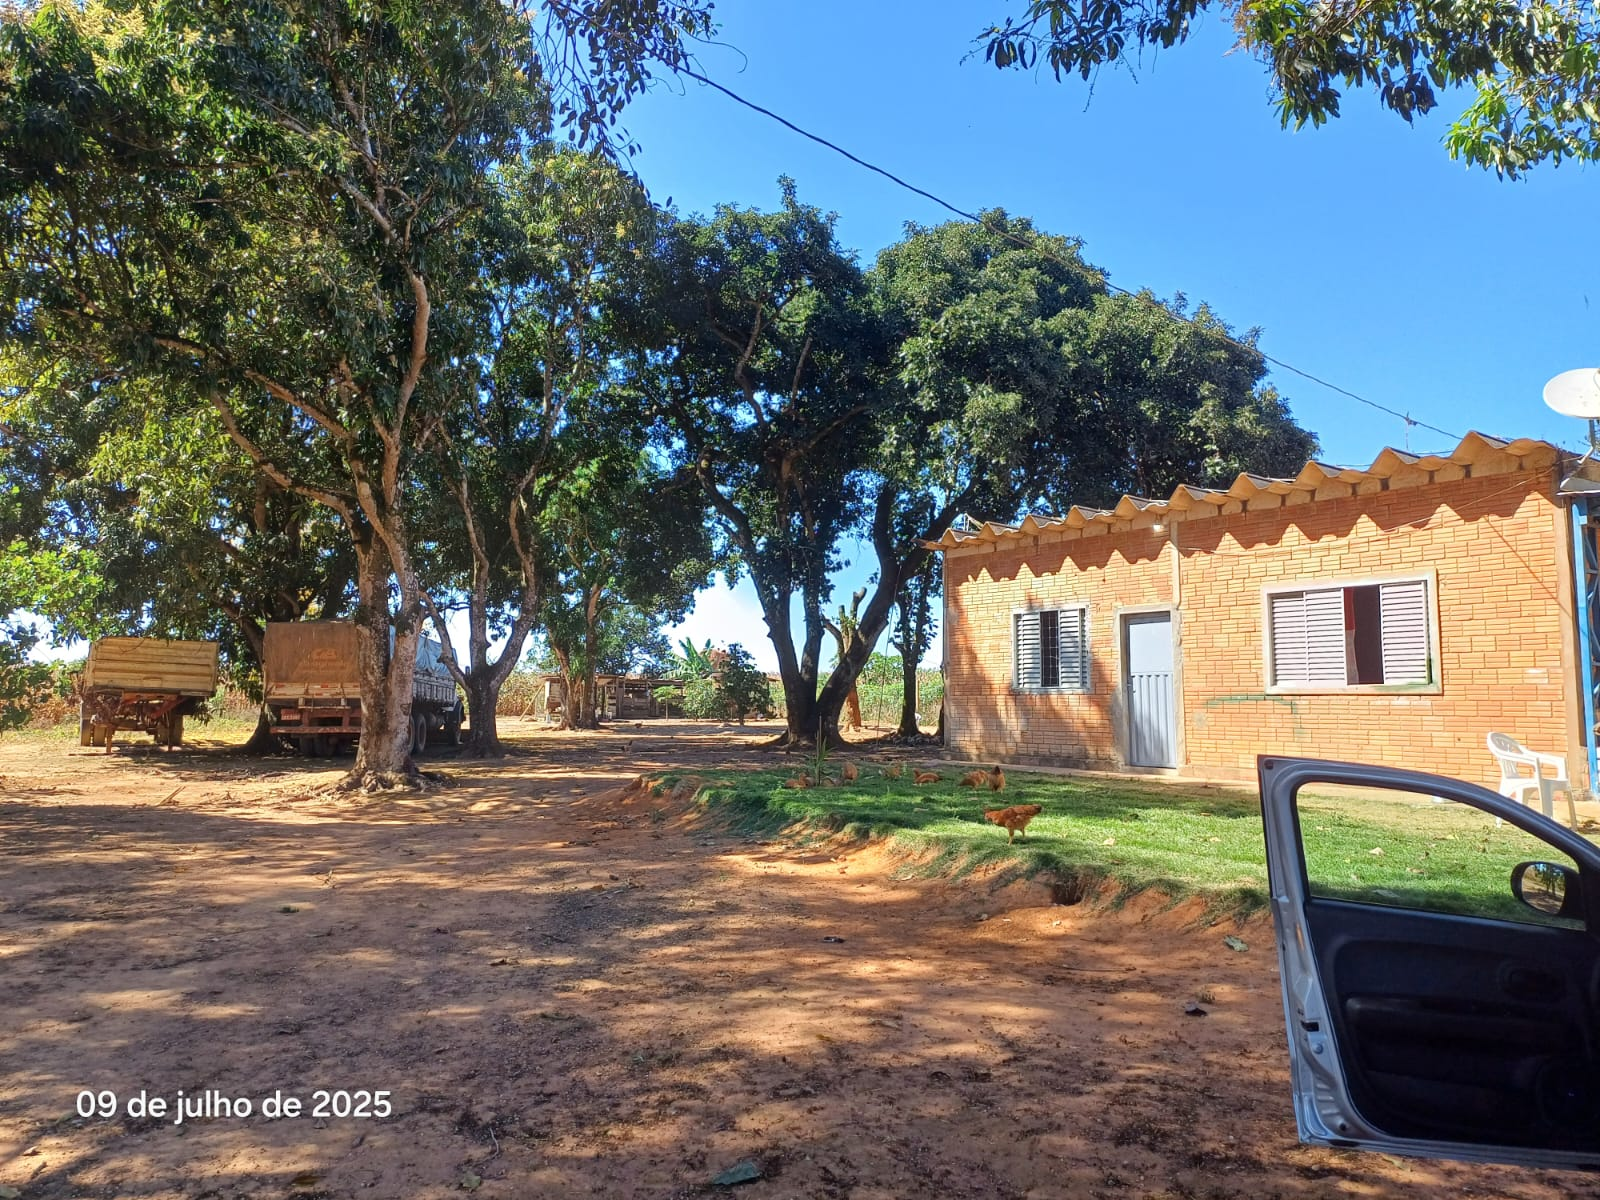
\includegraphics[width=0.49\linewidth]{./refs/Fotos/35} 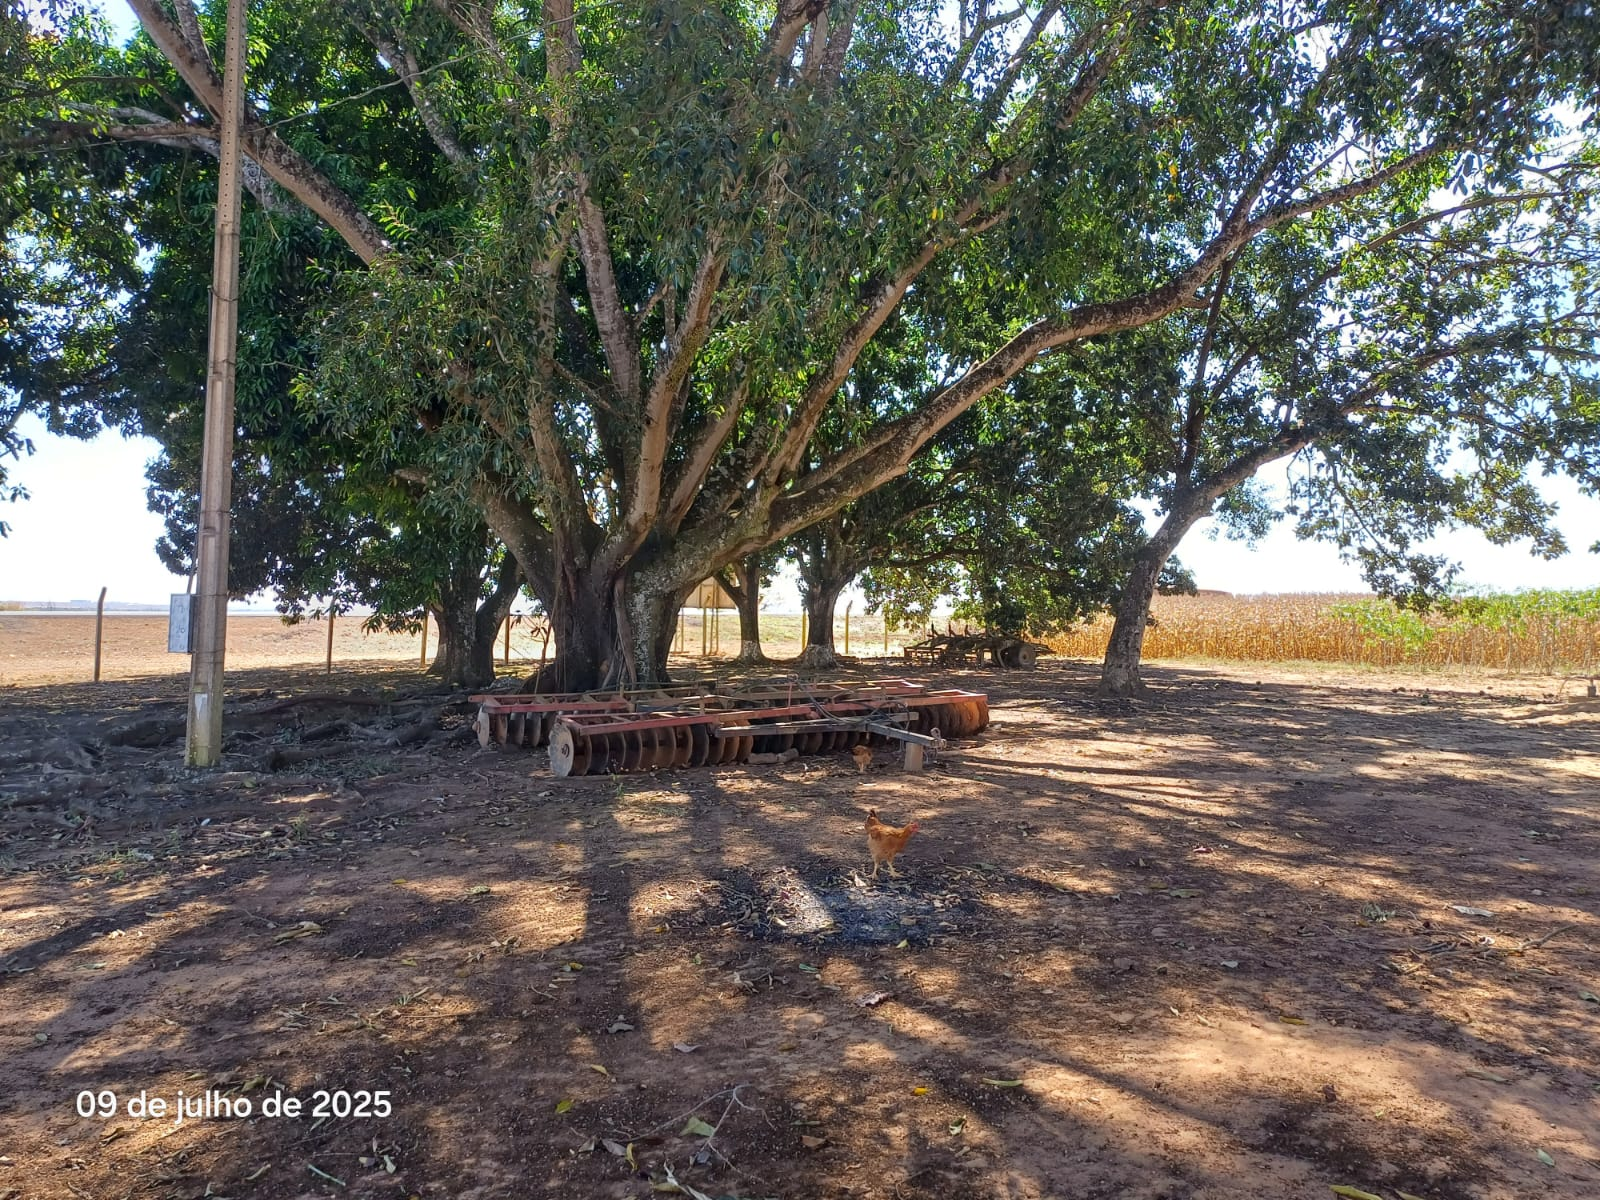
\includegraphics[width=0.49\linewidth]{./refs/Fotos/36} 

}

\caption{Sede.}\label{fig:Sede}
\end{figure}

\begin{figure}[H]

{\centering 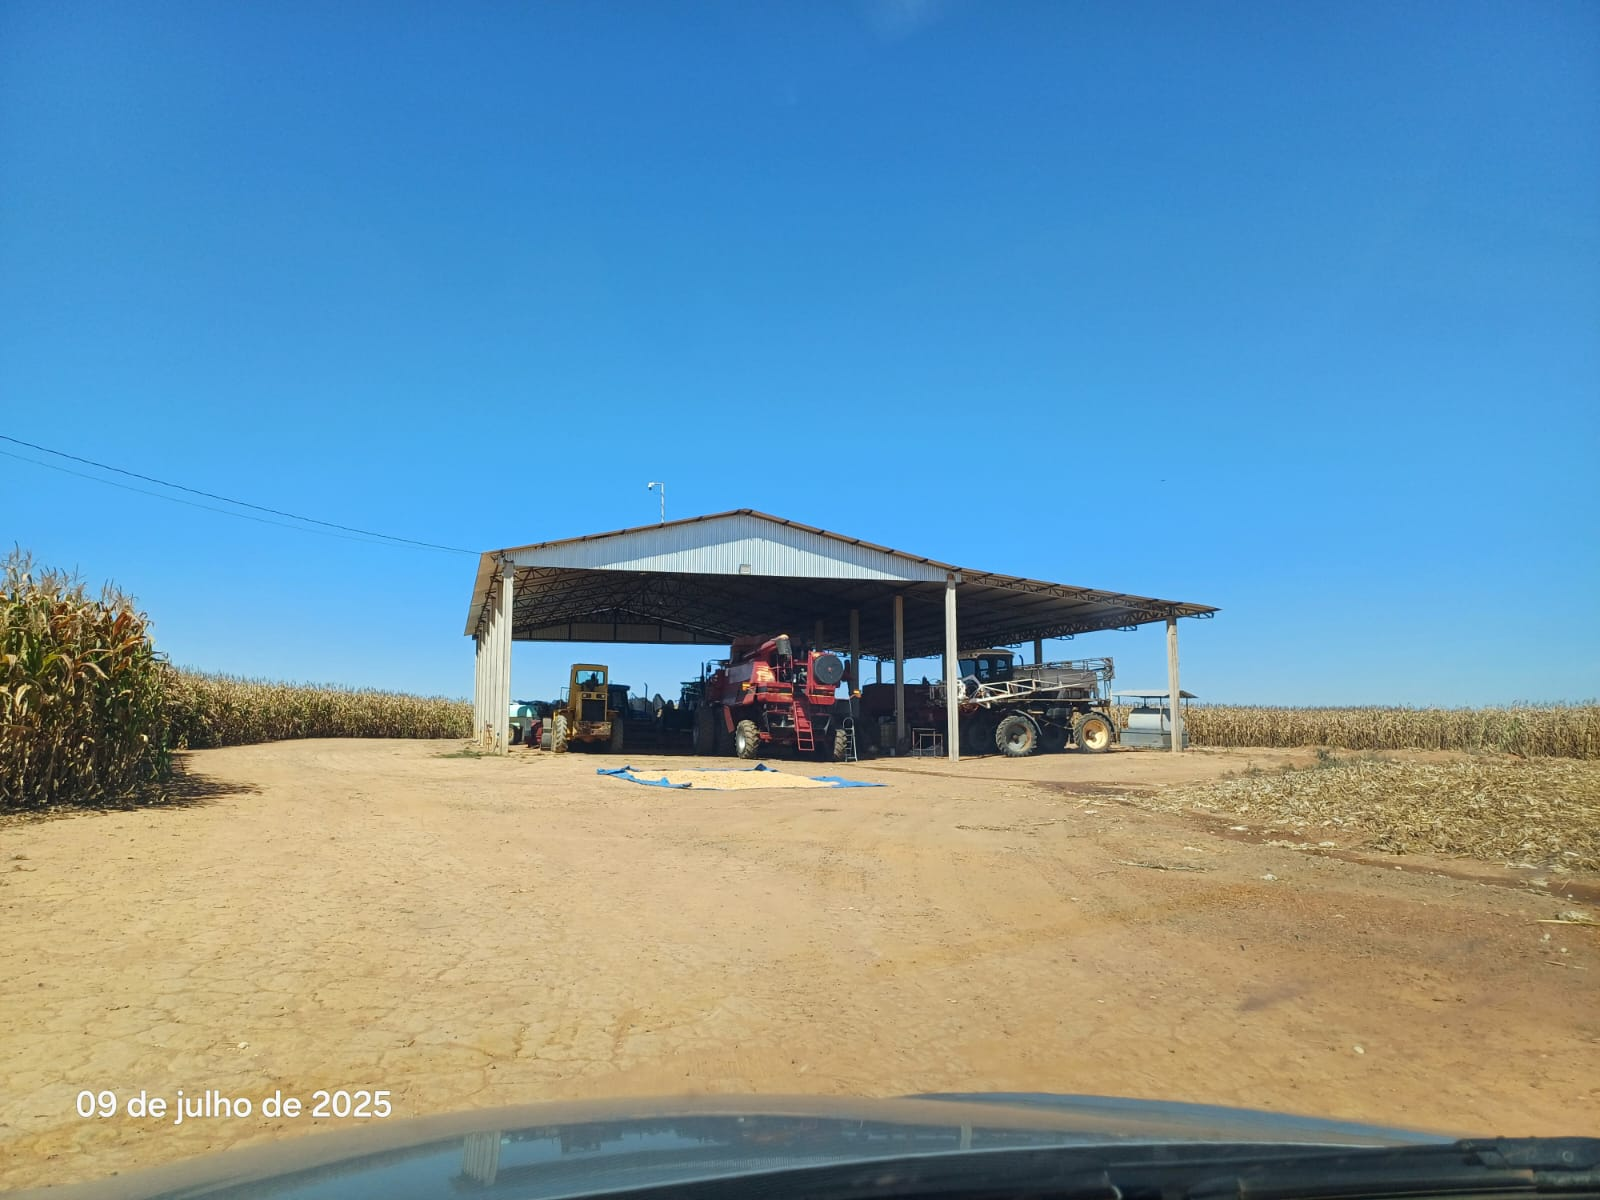
\includegraphics[width=0.49\linewidth]{./refs/Fotos/30} 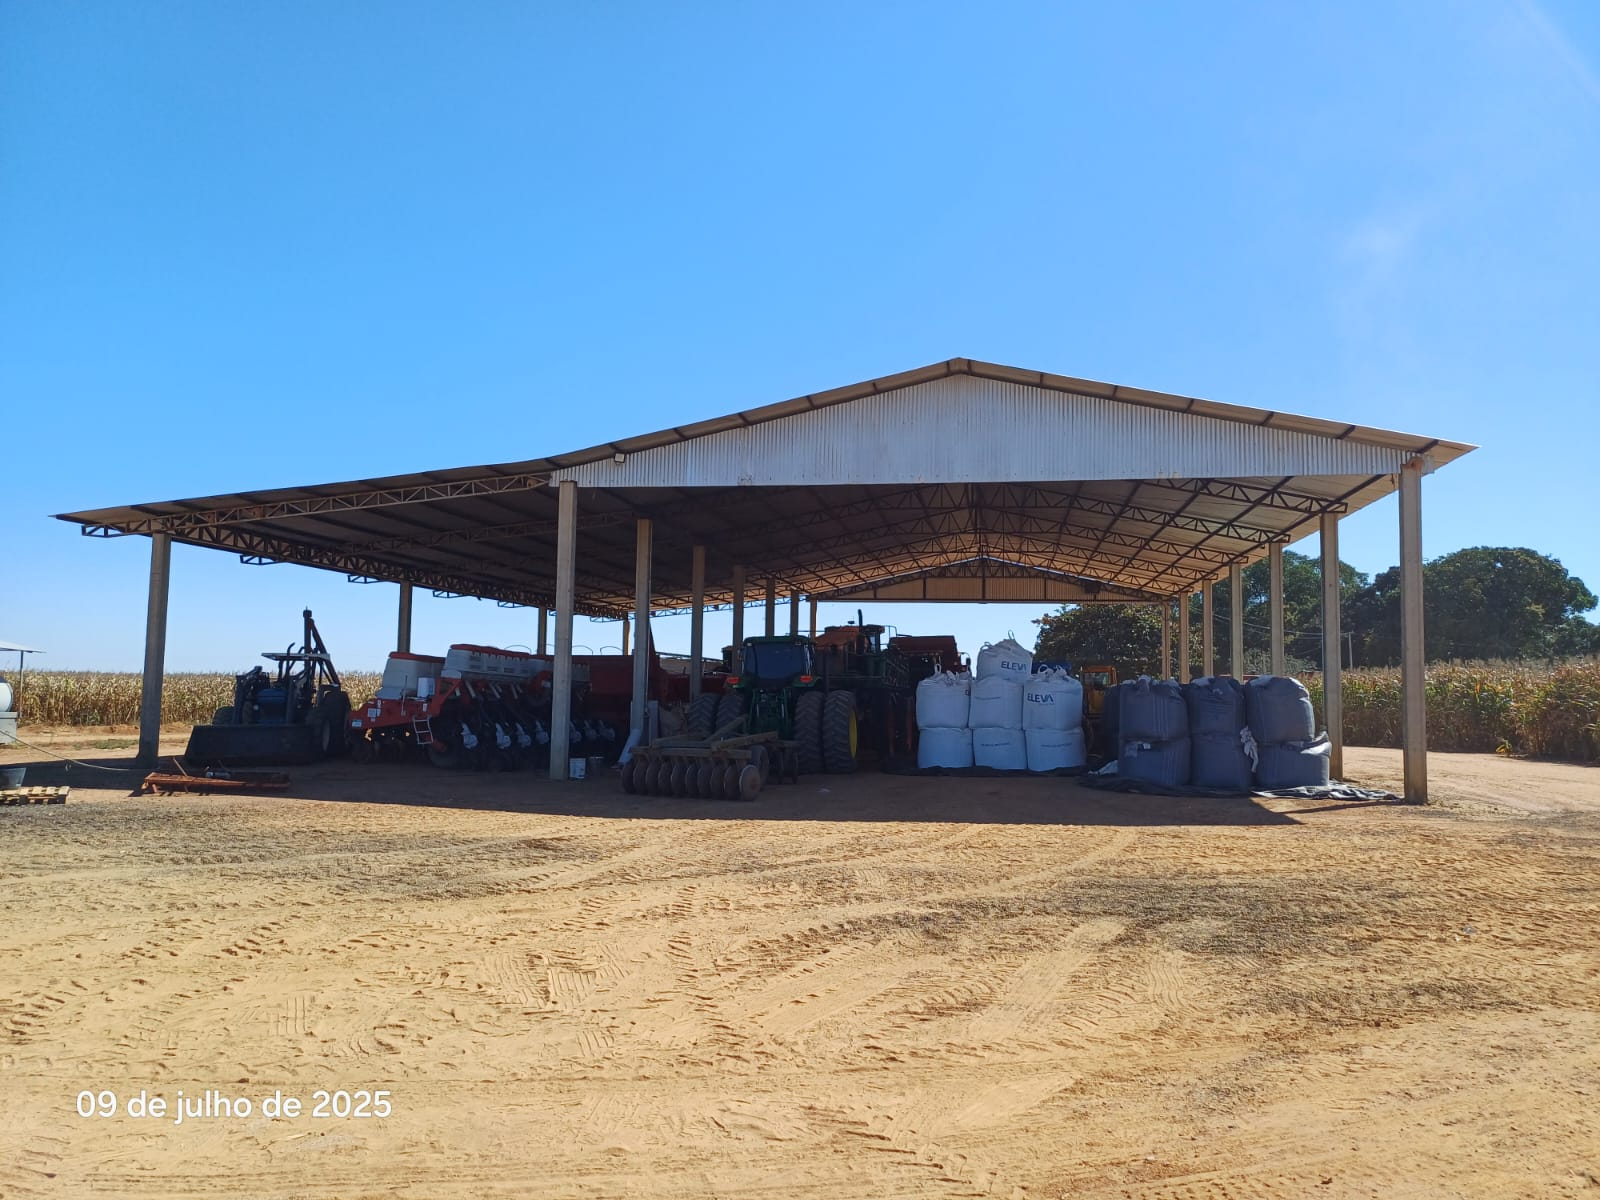
\includegraphics[width=0.49\linewidth]{./refs/Fotos/29} 

}

\caption{Barracão.}\label{fig:Barracao}
\end{figure}

\begin{figure}[H]

{\centering 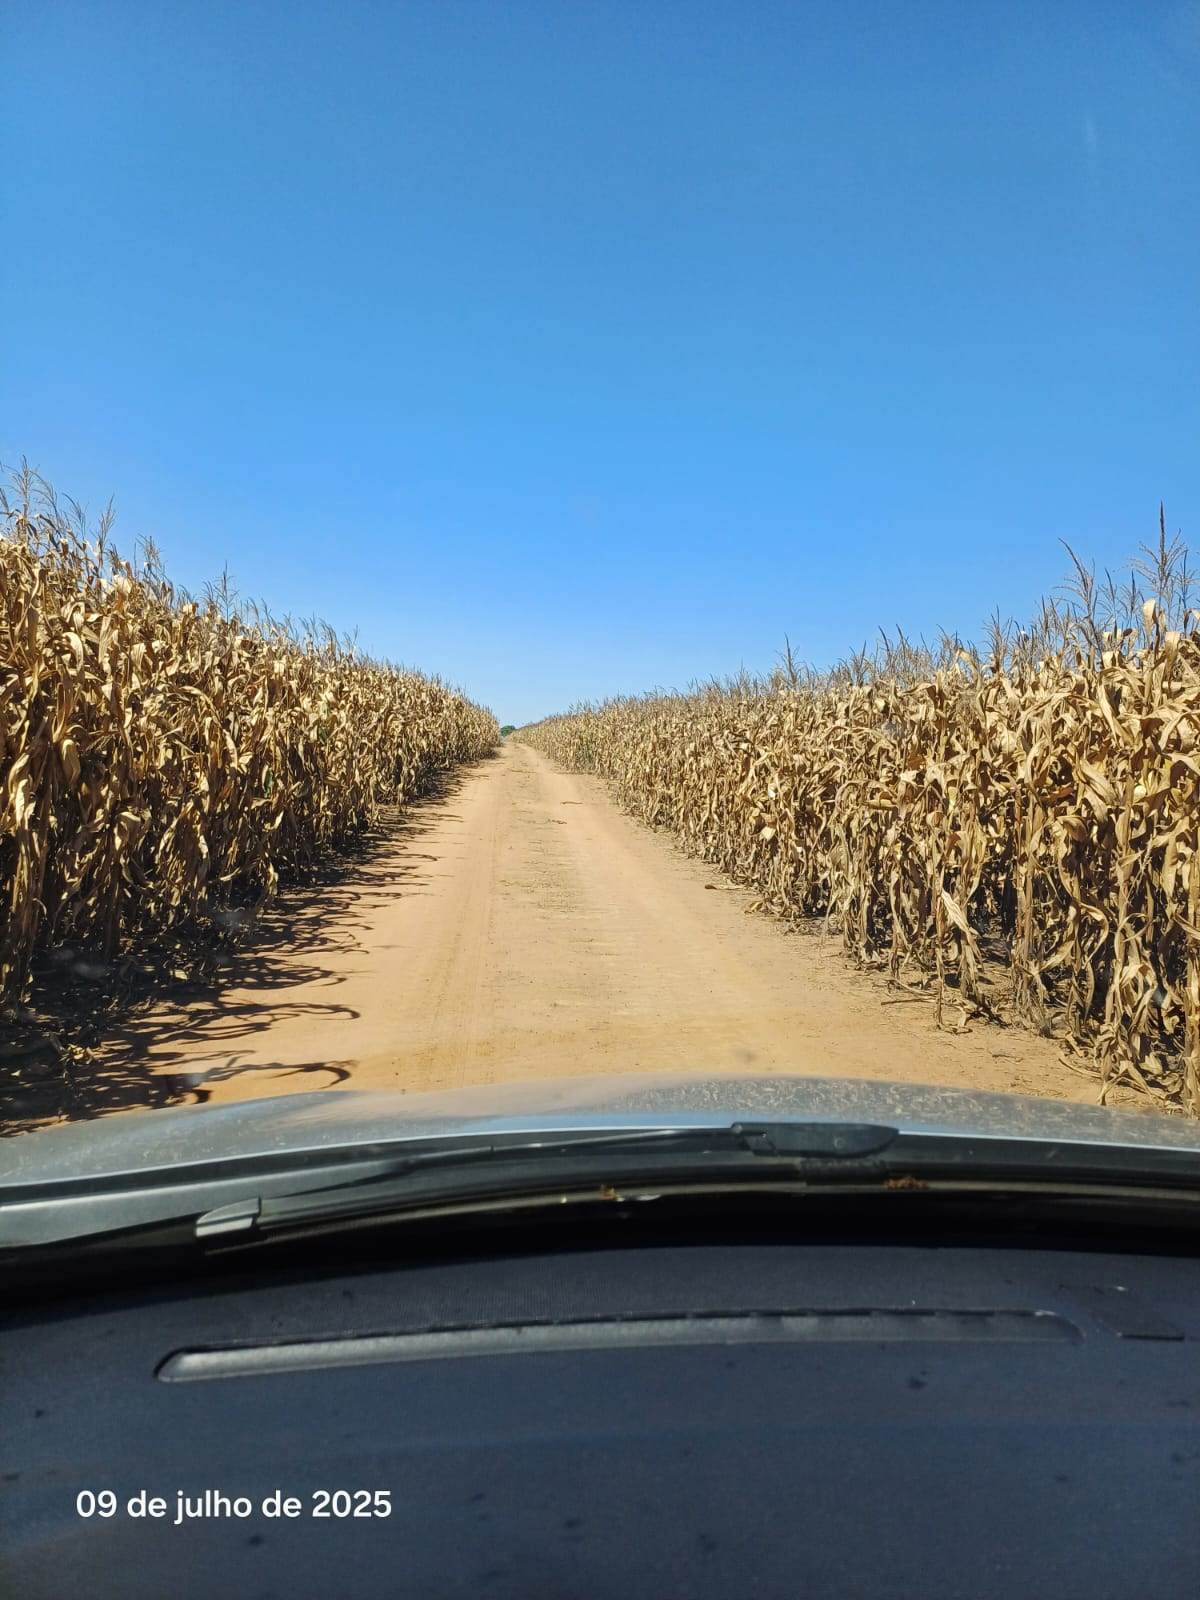
\includegraphics[width=0.49\linewidth]{./refs/Fotos/27} 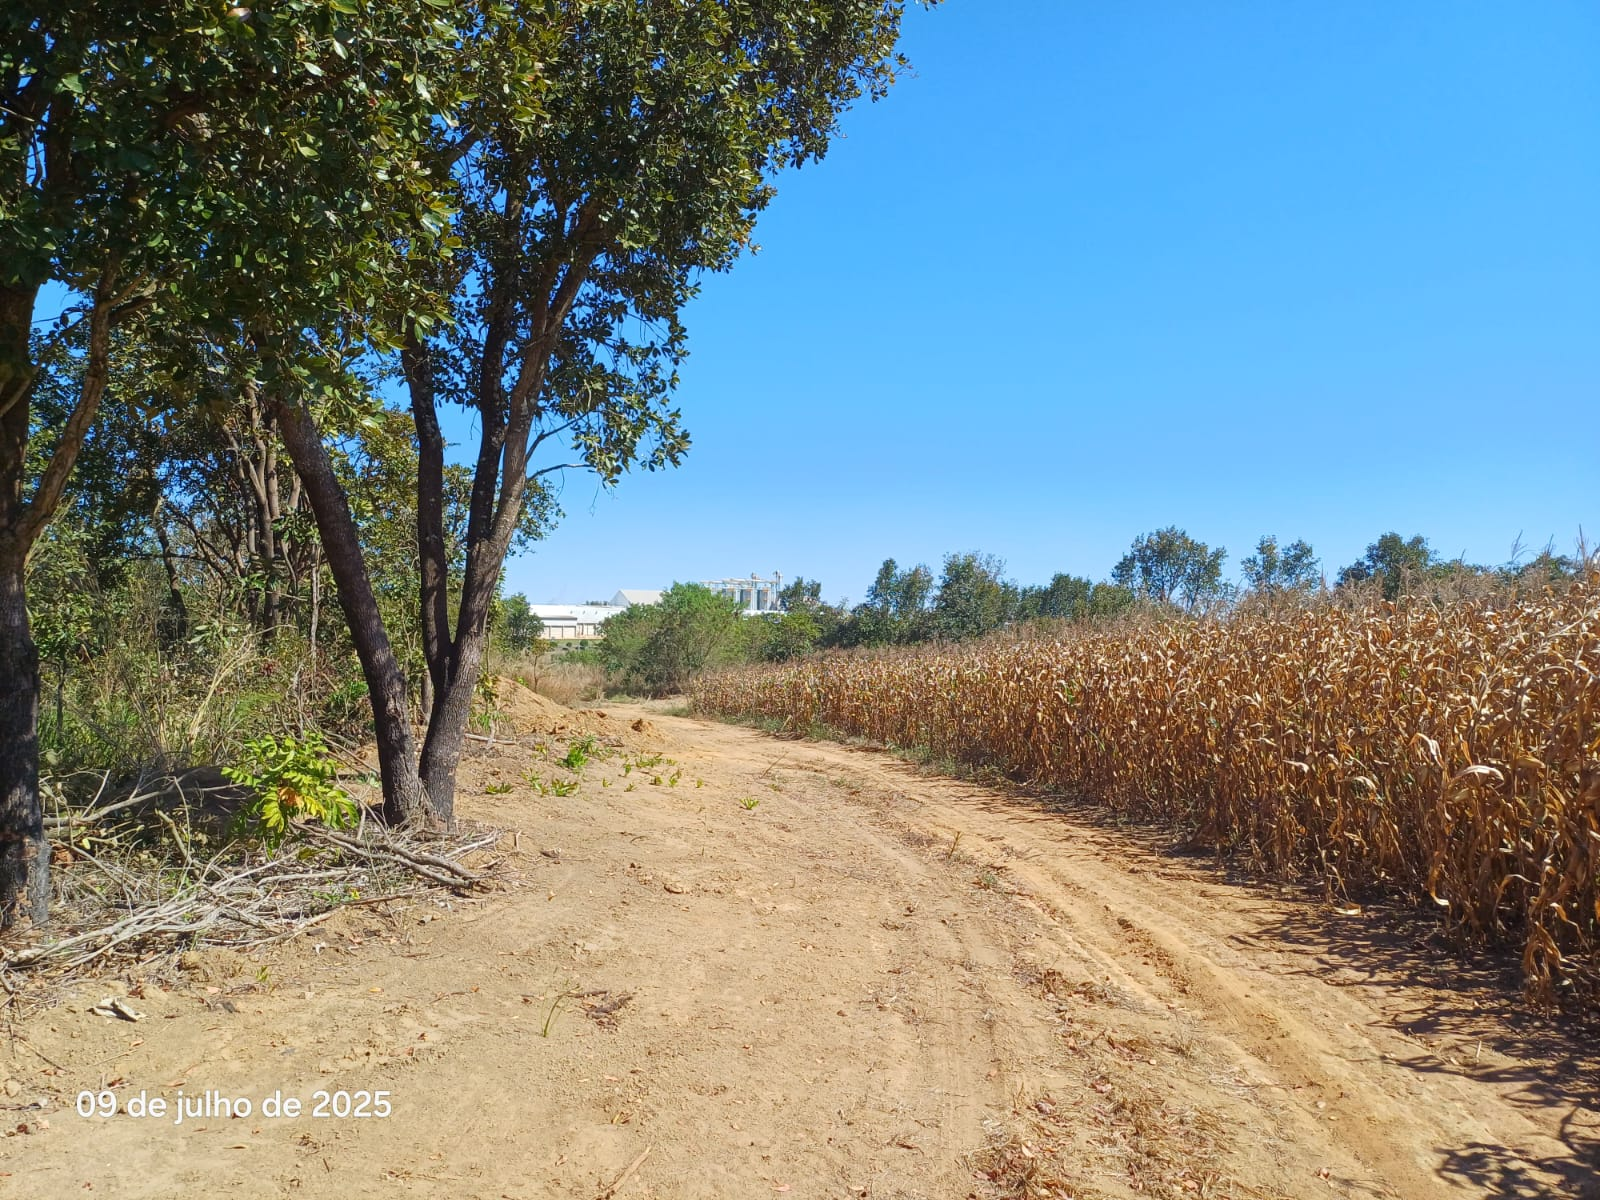
\includegraphics[width=0.49\linewidth]{./refs/Fotos/25} 

}

\caption{Carreadores internos.}\label{fig:Carreadores}
\end{figure}

\begin{figure}[H]

{\centering 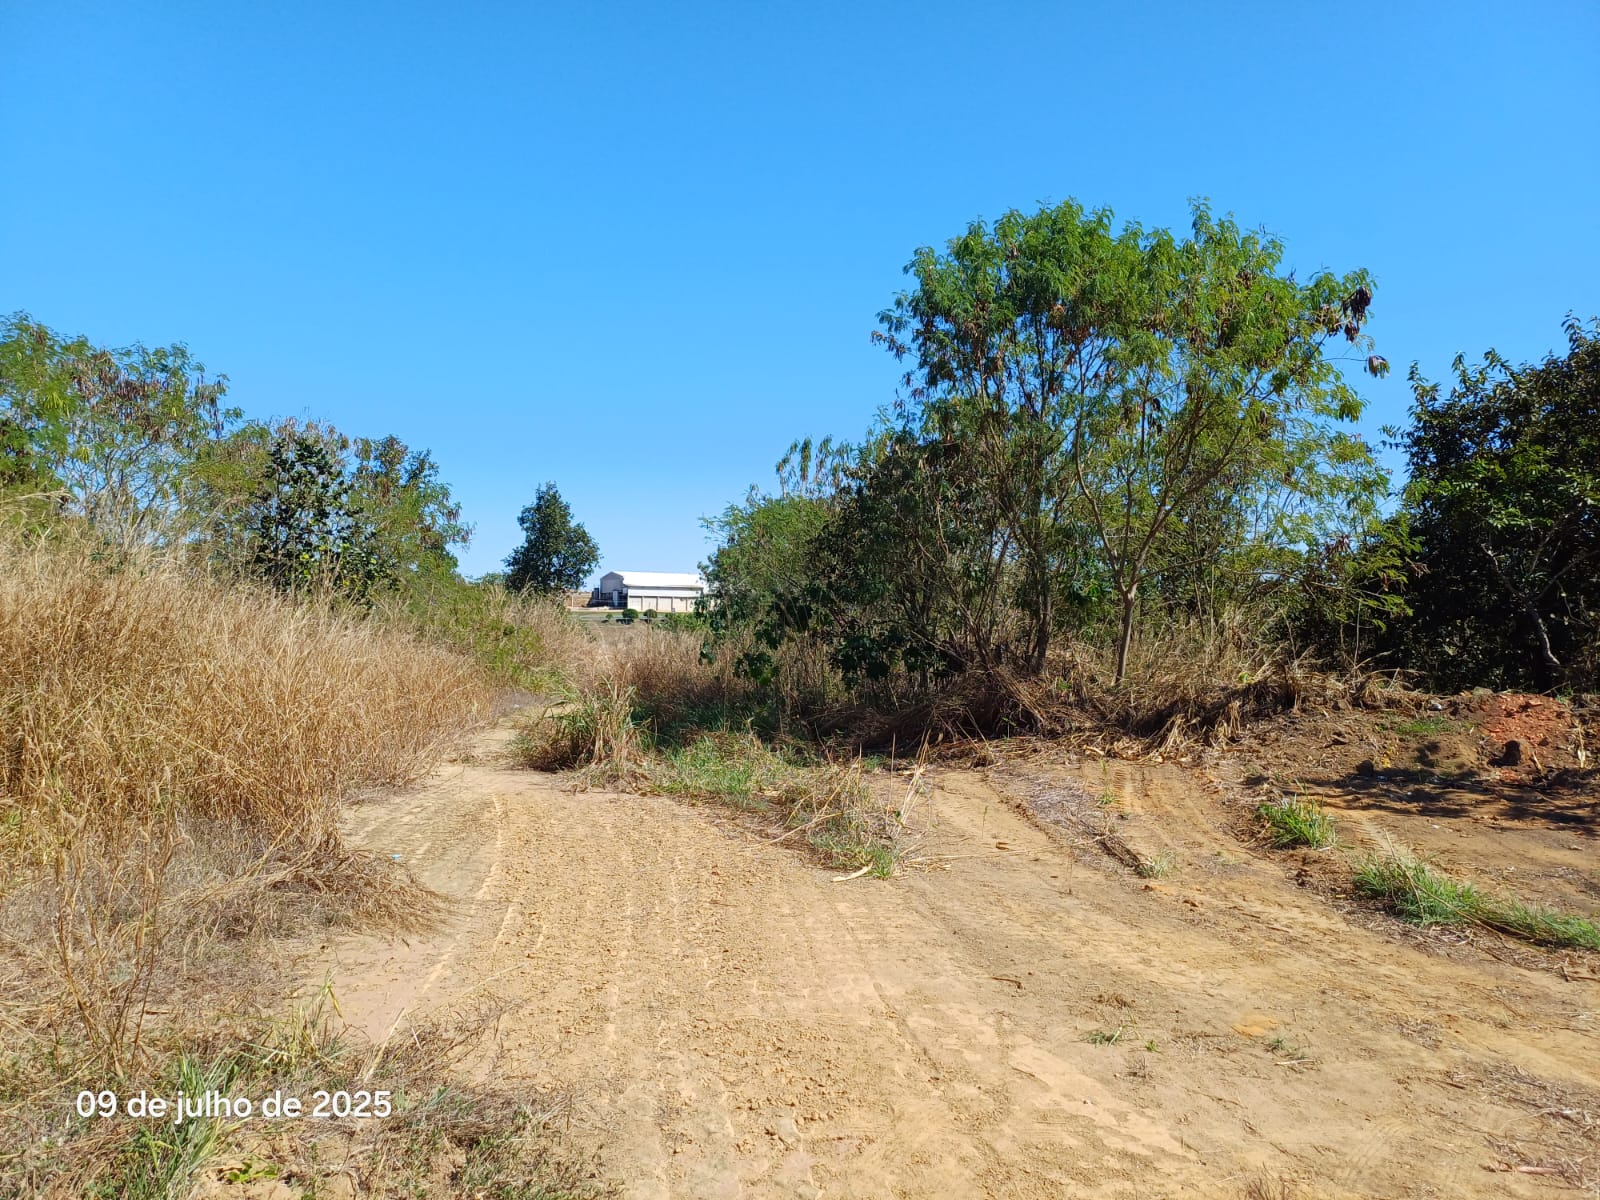
\includegraphics[width=0.49\linewidth]{./refs/Fotos/24} 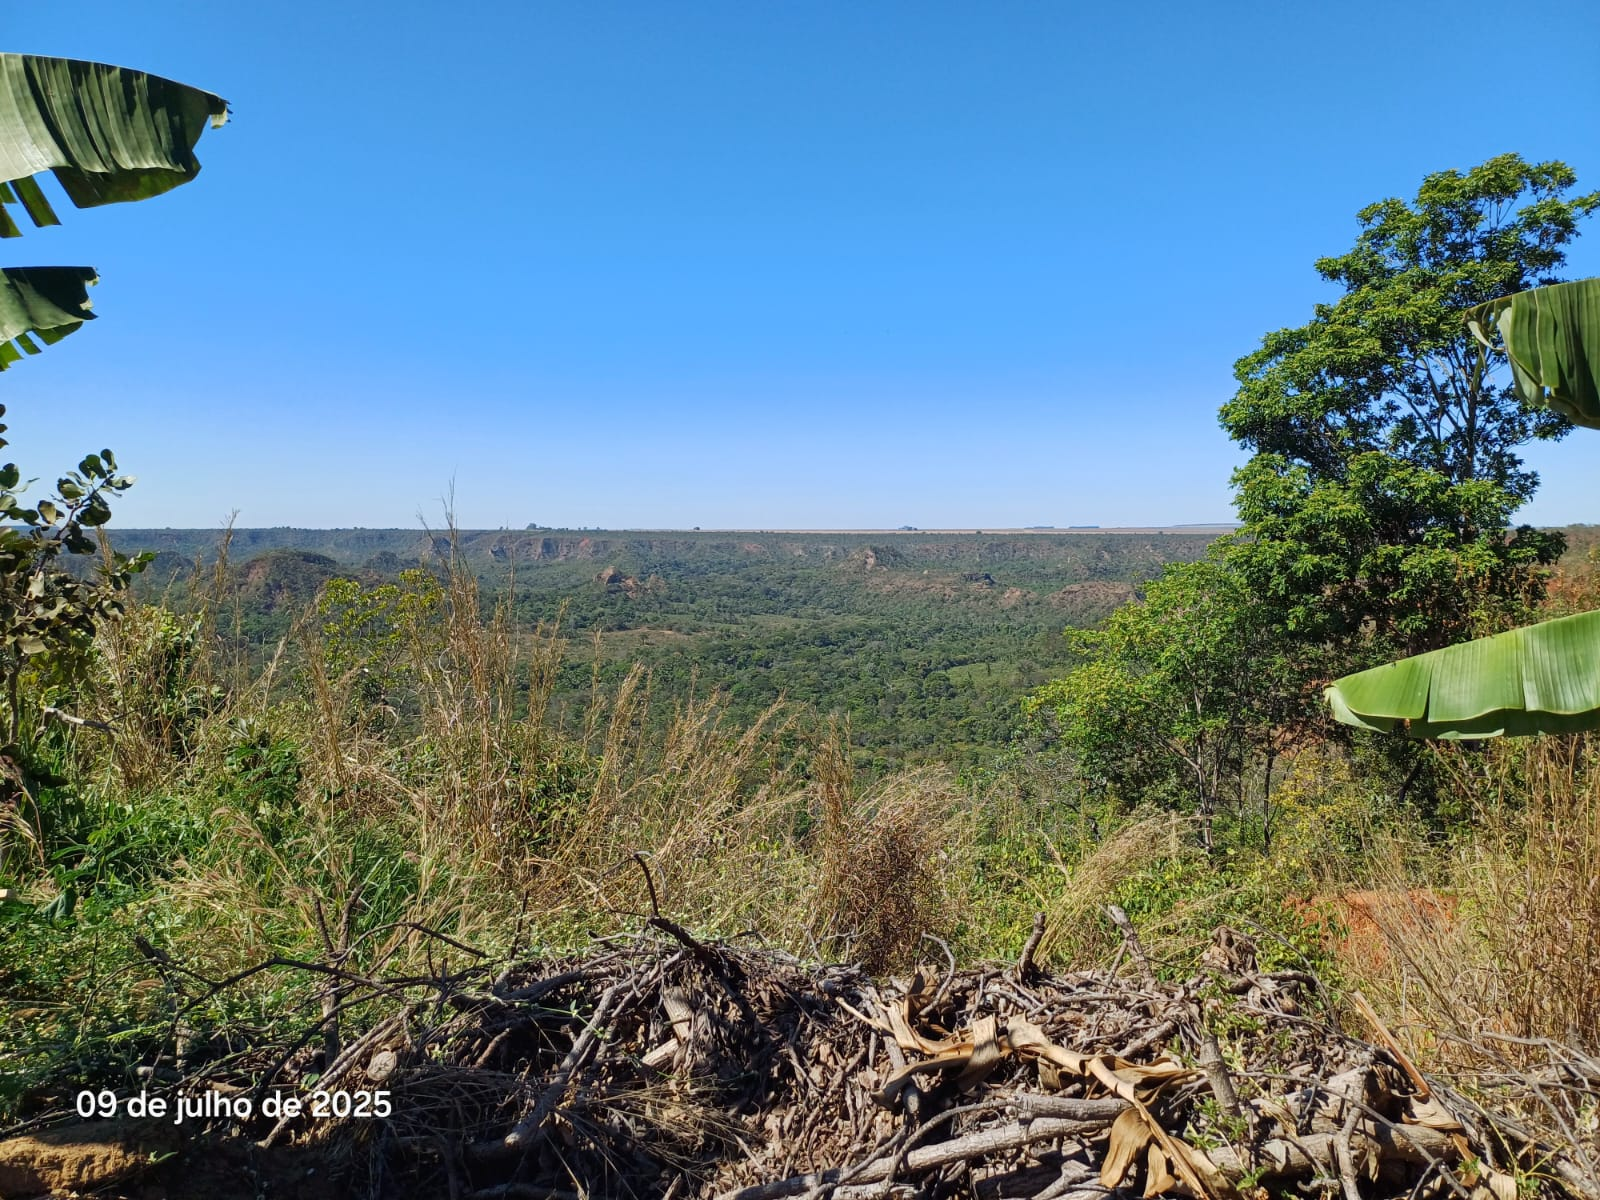
\includegraphics[width=0.49\linewidth]{./refs/Fotos/26} 

}

\caption{Vegetação esparsa/APP (Furnas).}\label{fig:Vegetacao}
\end{figure}

\section{Diagnóstico de Mercado}\label{diagnuxf3stico-de-mercado}

O imóvel está perfeitamente inserido no mercado de imóveis tipo lotes
industriais e/ou comerciais, encontrados no local, pois está localizado
nas imediações do distrito José de Alencar, importante distrito
industrial local. Sua localização é estratégica e tem facilidade de
acesso, especialmente por estar localizado às margens da Rodovia BR-070.

Quanto à expectativa do avaliador em relação ao desempenho do imóvel
avaliando no mercado, pode-se citar:

\begin{enumerate}
\def\labelenumi{\alph{enumi}.}
\tightlist
\item
  Quantidade de ofertas de bens similares: pequena em empreendimentos do
  tipo do projeto hipotético;
\item
  Público alvo para absorção do imóvel: pequenas, médias e grandes
  indústrias, além de possíveis investidores;
\item
  Desempenho de mercado: dada a conjuntura atual, com índices de
  inflação moderados, taxa de juros alta e expectativa de médio
  crescimento do PIB, o mercado de imóveis de maneira geral apresenta
  médio desempenho;
\item
  Absorção pelo mercado: a velocidade absorção do imóvel pelo mercado
  pode ser considerada de baixa à média;
\item
  Facilitadores para negociação do bem: localização estratégica e
  facilidade de acesso ao centro da cidade;
\item
  Liquidez: dadas as características do imóvel, público alvo e,
  principalmente da atual conjuntura econômica, um imóvel paradigma pode
  ser considerado de média liquidez.
\end{enumerate}

\section{Procedimentos
metodológicos}\label{procedimentos-metodoluxf3gicos}

\subsection{Métodos de avaliação}\label{muxe9todos-de-avaliauxe7uxe3o}

O método a ser usado numa avaliação, segunda a NBR 14653-1:2019, depende
da natureza do bem a ser avaliado e da finalidade da avaliação, da
qualidade e quantidade de informações coletadas no mercado imobiliário.
Sua escolha deve ser justificada, objetivando-se retratar o
comportamento do mercado por meio de modelos que expliquem seu valor.

Os métodos citados na NBR 14653-1:2019 são:

\begin{enumerate}
\def\labelenumi{\alph{enumi}.}
\tightlist
\item
  \textbf{Métodos para identificar o valor de um bem, de seus frutos e
  direitos}
\end{enumerate}

\begin{itemize}
\tightlist
\item
  \textbf{Método comparativo direto de dados de mercado:} Identifica o
  valor de mercado do bem por meio de tratamento técnico dos atributos
  dos elementos comparáveis, constituintes da amostra.
\item
  \textbf{Método involutivo:} estudo de viabilidade técnico-econômica,
  mediante hipotético empreendimento (que considere aproveitamento
  eficiente do terreno em avaliação) compatível com as características
  do bem e com as condições do mercado no qual está inserido,
  considerando-se cenários viáveis para execução e comercialização do
  produto.
\item
  \textbf{Método evolutivo:} Identifica o valor do bem pelo somatório
  dos valores de seus componentes. Caso a finalidade seja a
  identificação do valor de mercado, deve ser considerado o fator de
  comercialização.
\item
  \textbf{Método da capitalização da renda:} Identifica o valor do bem,
  com base na capitalização presente da sua renda líquida prevista,
  considerando-se cenários viáveis.
\end{itemize}

\begin{enumerate}
\def\labelenumi{\alph{enumi}.}
\setcounter{enumi}{1}
\tightlist
\item
  \textbf{Métodos para identificar o custo de um bem}
\end{enumerate}

\begin{itemize}
\tightlist
\item
  \textbf{Método comparativo direto de custo:} Identifica o custo do bem
  por meio de tratamento técnico dos atributos dos elementos
  comparáveis, constituintes da amostra.
\item
  \textbf{Método da quantificação de custo:} Identifica o custo do bem
  ou de suas partes por meio de orçamentos sintéticos ou analíticos a
  partir das quantidades de serviços e respectivos custos diretos e
  indiretos.
\end{itemize}

\begin{enumerate}
\def\labelenumi{\alph{enumi}.}
\setcounter{enumi}{2}
\tightlist
\item
  \textbf{Métodos para identificar indicadores de viabilidade da
  utilização econômica de um empreendimento}
\end{enumerate}

\begin{itemize}
\tightlist
\item
  Os procedimentos avaliatórios usuais com a finalidade de determinar
  indicadores de viabilidade da utilização econômica de um
  empreendimento são baseados no seu fluxo de caixa projetado, a partir
  do qual são determinados indicadores de decisão baseados no valor
  presente líquido, taxas internas de retorno, tempos de retorno, dentre
  outros.
\end{itemize}

A NBR 14.653-2:2011 (\citeproc{ref-NBR1465302}{ABNT, 2011}) em seu item
8.1.1 coloca que:

\epigraph{Para a identificação do valor de mercado, sempre que possível preferir
o método comparativo direto de dados de mercado (\ldots).}{NBR 14.653-02\\8.1.1}

\subsection{Método e Técnicas
Adotados}\label{muxe9todo-e-tuxe9cnicas-adotados}

Para a avaliação da gleba foi aplicado o método involutivo, considerando
um loteamento industrial hipotético.

As receitas do empreendimento foram obtidas a partir das vendas dos
lotes, baseadas no valor de mercado de um lote paradigma, cujo valor foi
obtido pelo método comparativo direto de dados de mercado usando a
técnica da regressão linear clássica.

Para o levantamento dos desembolsos necessários à urbanização da gleba
foi feito um orçamento usando custos paramétricos.

O modelo econômico-financeiro usado para avaliação da gleba será
detalhado a seguir.

\subsection{Método Involutivo}\label{muxe9todo-involutivo}

\subsubsection{Princípio}\label{princuxedpio}

O método involutivo baseia-se no estudo de viabilidade econômica de
aproveitamento de um terreno procurando determinar o valor do mesmo
através do estudo das condições máximas permissíveis e com
aproveitamento eficiente da área a ser futuramente utilizada.

O \emph{aproveitamento máximo} é o que as prefeituras municipais
permitem em seu Plano Diretor, limitado ao mesmo tempos simultaneamente
pela capacidade de absorção do mercado.

O \emph{aproveitamento eficiente} é a utilização mais adequada para o
local em questão (comercial, residencial, misto, industrial, \ldots).

\subsubsection{Roteiro de Aplicação}\label{roteiro-de-aplicauxe7uxe3o}

A NBR 14653-2:2011 apresenta as seguintes etapas para a aplicação do
método involutivo (item 8.2.2):

\begin{enumerate}
\def\labelenumi{\alph{enumi}.}
\tightlist
\item
  \textbf{Vistoria do imóvel}: caracterização de região, caracterização
  do terreno, caracterização das edificações e benfeitorias do entorno.
\item
  \textbf{Projeto hipotético}: Fazer um projeto de ocupação,
  considerando o máximo aproveitamento eficiente do terreno;
\item
  \textbf{Pesquisa de valores}: tem como objetivo estimar o valor de
  mercado do produto imobiliário (lote, apartamento, sala comercial,
  etc.) projetado e sua variação ao longo do tempo.
\item
  \textbf{Previsão de receitas}: são calculadas a partir da pesquisa de
  mercado, devendo-se considerar a eventual valorização imobiliária, a
  forma de comercialização e o tempo de absorção no mercado.
\item
  \textbf{Lançamento do custo de produção do PH}: corresponde à apuração
  dos custos diretos e indiretos. Principais itens a ser levado em
  conta:
\end{enumerate}

\begin{itemize}
\tightlist
\item
  Custos de aquisição e legalização do terreno (impostos e taxas
  cartoriais);
\item
  elaboração e aprovação do projeto;
\item
  custo da construção, incluindo o lucro do construtor;
\item
  Lucro do empreendimento (lucro da incorporação)
\end{itemize}

\begin{enumerate}
\def\labelenumi{\alph{enumi}.}
\setcounter{enumi}{5}
\tightlist
\item
  \textbf{Previsão de despesas adicionais. Exemplos}:
\end{enumerate}

\begin{itemize}
\tightlist
\item
  Publicidade;
\item
  Comercialização das unidades (corretagem).
\end{itemize}

\begin{enumerate}
\def\labelenumi{\alph{enumi}.}
\setcounter{enumi}{6}
\tightlist
\item
  \textbf{Margem de lucro do incorporador (item 8.2.2.7)}: Quando for
  usada margem de lucro, em modelos que não utilizem fluxo de caixa,
  esta deve ser considerada proporcional ao risco do empreendimento, que
  está diretamente ligado à quantidade de unidades resultantes do
  projeto, ao montante investido e ao prazo total previsto para retorno
  do capital. A margem de lucro adotada em modelos estáticos deve ter
  relação com o que é praticado no mercado.
\item
  \textbf{Prazos}: no caso de adoção de modelos dinâmicos, é recomendado
  que:
\end{enumerate}

\begin{itemize}
\tightlist
\item
  o prazo para a execução do projeto hipotético seja compatível com as
  suas características físicas, disponibilidade de recursos, tecnologia
  e condições mercadológicas;
\item
  o prazo para a venda das unidades seja compatível com o mercado.
\end{itemize}

\begin{enumerate}
\def\labelenumi{\roman{enumi}.}
\tightlist
\item
  \textbf{Taxas}: No caso de adoção de modelos dinâmicos recomenda-se
  explicitar as taxas de valorização imobiliária, de evolução de custos
  e despesas, de juros do capital investido e a mínima de atratividade.
\end{enumerate}

\begin{enumerate}
\def\labelenumi{\alph{enumi}.}
\setcounter{enumi}{9}
\tightlist
\item
  \textbf{Modelo}: o valor do terreno é obtido pela diferença entre as
  receitas e o total de custos e despesas. A avaliação poderá ser
  realizada com a utilização dos seguintes modelos, em ordem de
  preferência:
\end{enumerate}

\begin{itemize}
\tightlist
\item
  Por fluxos de caixa específicos;
\item
  com a aplicação de modelos simplificados dinâmicos;
\item
  com a aplicação de modelos estáticos.
\end{itemize}

\section{Construção do Modelo
Econômico-Financeiro}\label{construuxe7uxe3o-do-modelo-econuxf4mico-financeiro}

Serão detalhados neste item todos os procedimentos usados para a
construção do modelo econômico-financeiro usado para avaliar a gleba.

\subsection{Software utilizados}\label{software-utilizados}

Foi elaborado um
\href{https://valoristica.github.io/PrimaveraLeste/}{Sistema de
Informações Geográficas (SIG)} em linguagem \emph{JavaScript}, em
conjunto com a biblioteca \href{https://leafletjs.com/}{leaflet}, após a
confecção das camadas realizada com o auxílio \emph{software} livre
QGIS, contendo o anteprojeto do loteamento hipotético.

Todos os outros cálculos foram efetuados na linguagem \textsf{R}, versão
4.4.2.

\subsection{Projeto de Loteamento
Hipotético}\label{projeto-de-loteamento-hipotuxe9tico}

Um Projeto Hipotético (PH) foi elaborado com nível de detalhe suficiente
para prever o fluxo de caixa do projeto. Não faz parte do escopo deste
trabalho a construção de um projeto de loteamento detalhado,
contemplando a localização exata de todos os lotes, áreas
institucionais, arruamentos precisos, etc.

A Figura \ref{fig:PH} apresenta, portanto, um estudo preliminar do
projeto hipotético considerado. Nesta Figura, em verde-escuro podem ser
vistas as áreas verdes a serem preservadas, representando aprox. 23\% da
área total da gleba; em amarelo-escuro podem ser vistas as áreas a serem
destinadas para a construção de lotes (quadras), representando aprox.
67\% da área total da gleba. Por fim, as áreas institucionais foram
consideradas diluídas nos arruamentos, que representam aprox. 11\% da
área total da gleba.

Deste estudo preliminar foram obtidas as áreas apresentadas na Tabela 1
abaixo:

\begin{longtable}[]{@{}lrr@{}}
\caption{Subdivisão do loteamento hipotético.}\tabularnewline
\toprule\noalign{}
Descrição & Área (m2) & Proporção \\
\midrule\noalign{}
\endfirsthead
\toprule\noalign{}
Descrição & Área (m2) & Proporção \\
\midrule\noalign{}
\endhead
\bottomrule\noalign{}
\endlastfoot
Áreas Verdes e de lazer & 696.176 & 22,03\% \\
Áreas dos Lotes (útil) & 2.130.000 & 67,41\% \\
Árruamentos e outros & 333,55 & 0,011\% \\
\end{longtable}

A Tabela 1 mostra que 67,41\% da área da gleba podem ser transformados
em lotes, totalizando assim 2.130.000 \(m^2\) de área vendável.
Considerando um lote paradigma de 15.000 \(m^2\), esta área resulta em
142 lotes disponíveis para venda.

\begin{figure}[H]

{\centering \includegraphics[width=0.7\linewidth]{images/PH-1} 

}

\caption{Projeto Hipotético.}\label{fig:PH}
\end{figure}

Devido ao grande número de lotes, o fluxo de caixa do empreendimento
será dividido em 3 etapas de vendas, sendo as duas primeiras com duração
de 17 meses cada e a terceira com 14 meses. Considerou-se ainda que os
lotes começarão a ser vendidos após 11 meses do início do projeto.

Na primeira etapa serão vendidos 50 lotes, na segunda etapa serão
vendidos outros 50 e, por fim, na terceira etapa serão vendidos 42
lotes. A velocidade de venda de 3 lotes mensais foi adotada. A duração
total do empreendimento resultou em 59 meses.

As Figuras \ref{fig:Etapa1} a \ref{fig:Etapas2-3} mostram como foram
definidas as etapas do loteamento. Na Primeira Etapa serão urbanizados e
vendidos 50 lotes situados nas quadras adjacentesaos lotes industriais
existentes no distrito industrial lindeiro. Na Segunda Etapa serão
comercializados mais 50 lotes que se encontram na área central da
propriedade, nas proximidades da atual porteira de acesso principal da
propriedade. Já na 3ª e última etapa são considerados 42 lotes residuais
encontrados nas quadras situadas mais distantes da região central de
Primavera do Leste.

\begin{figure}[H]

{\centering \includegraphics[width=0.7\linewidth]{images/Etapa1-1} 

}

\caption{Etapa 1.}\label{fig:Etapa1}
\end{figure}

\begin{figure}[H]

{\centering \includegraphics[width=0.49\linewidth]{images/Etapas2-3-1} \includegraphics[width=0.49\linewidth]{images/Etapas2-3-2} 

}

\caption{Etapas 2 e 3.}\label{fig:Etapas2-3}
\end{figure}

\subsection{Estimativa de Receitas}\label{estimativa-de-receitas}

O valor de cada lote paradigma, conforme apresentado no
\hyperref[anexo-i]{ANEXO I} (Laudo do Método Comparativo Direto de Dados
de Mercado), é R\$ 3.750.000. A Tabela 2 apresenta um resumo das
estimativas de receitas por etapa e do Valor Global de Vendas (VGV).

\begin{longtable}[]{@{}lrr@{}}
\caption{Estimativas de Receitas por Etapa}\tabularnewline
\toprule\noalign{}
ETAPA & LOTES & RECEITA (R\$) \\
\midrule\noalign{}
\endfirsthead
\toprule\noalign{}
ETAPA & LOTES & RECEITA (R\$) \\
\midrule\noalign{}
\endhead
\bottomrule\noalign{}
\endlastfoot
1ª Etapa & 50 & 150.000.000,00 \\
2ª Etapa & 50 & 150.000.000,00 \\
3ª Etapa & 42 & 126.000.000,00 \\
\end{longtable}

\subsection{Estimativas de Custos de
Urbanização}\label{estimativas-de-custos-de-urbanizauxe7uxe3o}

Para a estimativa dos custos de urbanização foram usados custos
publicados pela PINI, que apresenta valores unitários para 1.000 m2 de
área útil do loteamento. O \hyperref[anexo-ii]{ANEXO II} apresenta uma
tabela destes valores.

A Tabela 3 apresenta os custos de urbanização para as diferentes etapas
consideradas.

\begin{longtable}[]{@{}
  >{\raggedright\arraybackslash}p{(\linewidth - 8\tabcolsep) * \real{0.5052}}
  >{\raggedleft\arraybackslash}p{(\linewidth - 8\tabcolsep) * \real{0.1237}}
  >{\raggedleft\arraybackslash}p{(\linewidth - 8\tabcolsep) * \real{0.1237}}
  >{\raggedleft\arraybackslash}p{(\linewidth - 8\tabcolsep) * \real{0.1237}}
  >{\raggedleft\arraybackslash}p{(\linewidth - 8\tabcolsep) * \real{0.1237}}@{}}
\caption{Custo de urbanização por 1.000 m2 de área útil.}\tabularnewline
\toprule\noalign{}
\begin{minipage}[b]{\linewidth}\raggedright
SERVIÇO
\end{minipage} & \begin{minipage}[b]{\linewidth}\raggedleft
CUSTO PINI
\end{minipage} & \begin{minipage}[b]{\linewidth}\raggedleft
1ª ETAPA
\end{minipage} & \begin{minipage}[b]{\linewidth}\raggedleft
2ª ETAPA
\end{minipage} & \begin{minipage}[b]{\linewidth}\raggedleft
3ª ETAPA
\end{minipage} \\
\midrule\noalign{}
\endfirsthead
\toprule\noalign{}
\begin{minipage}[b]{\linewidth}\raggedright
SERVIÇO
\end{minipage} & \begin{minipage}[b]{\linewidth}\raggedleft
CUSTO PINI
\end{minipage} & \begin{minipage}[b]{\linewidth}\raggedleft
1ª ETAPA
\end{minipage} & \begin{minipage}[b]{\linewidth}\raggedleft
2ª ETAPA
\end{minipage} & \begin{minipage}[b]{\linewidth}\raggedleft
3ª ETAPA
\end{minipage} \\
\midrule\noalign{}
\endhead
\bottomrule\noalign{}
\endlastfoot
Topografia & 12.060,06 & 100\% & 100\% & 100\% \\
Terraplanagem leve & 2.078,35 & 100\% & 100\% & 100\% \\
Terraplanagem média & 5.968,19 & 0\% & 0\% & 0\% \\
Terraplanagem pesada & 15.693,02 & 0\% & 0\% & 0\% \\
Rede de água potável & 11.959,62 & 100\% & 100\% & 100\% \\
Rede de Esgoto & 28.885,35 & 100\% & 100\% & 100\% \\
Drenagem de Águas pluviais: galerias & 11.881,14 & 100\% & 100\% &
100\% \\
Drenagem de Águas pluviais: guias e sarjetas & 9.786,87 & 100\% & 100\%
& 100\% \\
Pavimentação & 31.994,26 & 100\% & 100\% & 100\% \\
Rede de Iluminação Pública & 3.880,58 & 100\% & 100\% & 100\% \\
CUSTO TOTAL & - & 112.526,23 & 112.526,23 & 112.526,23 \\
\end{longtable}

Como o loteamento em questão possui diversas quadras que ficam defronte
à Rodovia BR-070, e o proprietário pode vender estas quadras de maneira
integral para grandes indústrias, considerou-se neste laudo que a
urbanização se dará apenas nas quadras internas do loteamento.

A Tabela 4 mostra um resumo dos custos totais de urbanização por etapa.

\begin{longtable}[]{@{}lrrr@{}}
\caption{Estimativas de Custos de Urbanização por Etapa}\tabularnewline
\toprule\noalign{}
ETAPA & LOTES & ÁREA ÚTIL (M2) & CUSTOS (R\$) \\
\midrule\noalign{}
\endfirsthead
\toprule\noalign{}
ETAPA & LOTES & ÁREA ÚTIL (M2) & CUSTOS (R\$) \\
\midrule\noalign{}
\endhead
\bottomrule\noalign{}
\endlastfoot
1ª Etapa & 30 & 450.000,00 & 50.636.803,50 \\
2ª Etapa & 37 & 555.000,00 & 62.452.057,65 \\
3ª Etapa & 17 & 255.000,00 & 28.694.188,65 \\
TOTAL & 84 & 2.130.000,00 & 141.783.049,80 \\
\end{longtable}

\subsection{Benefícios e Despesas
Indiretas}\label{benefuxedcios-e-despesas-indiretas}

Para os benefícios e despesas indiretas (BDI) do urbanizador será
adotada a taxa de 23,02\%, atendendo o Acórdão nº 2622/2013 do Tribunal
de Contas da União (TCU) que estabelece valores de BDI por tipos de
obras públicas e para aquisição de materiais e equipamentos.

Como não existe especificada a atividade do loteador neste acórdão,
fez-se uma média ponderada pelos custos atribuídos às atividades ali
especificadas. Os custos são aqueles apresentados na Tabela 3, sendo que
os custos dos serviços de topografia são divididos pela metade entre as
atividades \say{construção 
de rodovias} e \say{redes de abastecimento de água e coleta de esgoto}
constantes no referido acórdão. A Tabela 5 apresenta os resultados desta
ponderação.

\begin{longtable}[]{@{}lrrrr@{}}
\caption{Determinação do BDI do Urbanizador.}\tabularnewline
\toprule\noalign{}
SERVIÇO & BDI ACÓRDÃO & CUSTOS & PESO & BDI URB. \\
\midrule\noalign{}
\endfirsthead
\toprule\noalign{}
SERVIÇO & BDI ACÓRDÃO & CUSTOS & PESO & BDI URB. \\
\midrule\noalign{}
\endhead
\bottomrule\noalign{}
\endlastfoot
RODOVIAS & 20,97\% & 40.102,64 & 0,356 & 7,47\% \\
REDES (ÁGUAS + ESGOTO) & 24,18\% & 68.543,01 & 0,609 & 14,73\% \\
REDE ELÉTRICA & 25,84\% & 3.880,58 & 0,034 & 0,89\% \\
TOTAL & - & 112.526,23 & 1,00 & 23,09\% \\
\end{longtable}

A parcela de lucros (benefícios) não foi considerada para o loteador
(empreendedor), pois seus benefícios foram contemplados na taxa usada
para descontar o fluxo de caixa (FC). A Tabela 6 mostra a determinação
das despesas indiretas do loteador para os componentes administração
central, seguros mais garantias e despesas financeiras. Foram
considerados os valores do primeiro quartil sugeridos no Acórdão nº
2622/2013 (TCU), adaptando desta forma estes custos para o loteador, que
tem uma estrutura gerencial mais enxuta. A ponderação foi efetuada
usando-se os mesmos pesos apresentados na Tabela 5.

\begin{longtable}[]{@{}
  >{\raggedright\arraybackslash}p{(\linewidth - 10\tabcolsep) * \real{0.2841}}
  >{\raggedleft\arraybackslash}p{(\linewidth - 10\tabcolsep) * \real{0.1591}}
  >{\raggedleft\arraybackslash}p{(\linewidth - 10\tabcolsep) * \real{0.2159}}
  >{\raggedleft\arraybackslash}p{(\linewidth - 10\tabcolsep) * \real{0.1591}}
  >{\raggedleft\arraybackslash}p{(\linewidth - 10\tabcolsep) * \real{0.0795}}
  >{\raggedleft\arraybackslash}p{(\linewidth - 10\tabcolsep) * \real{0.1023}}@{}}
\caption{Despesas Indiretas do Loteador.}\tabularnewline
\toprule\noalign{}
\begin{minipage}[b]{\linewidth}\raggedright
SERVIÇO
\end{minipage} & \begin{minipage}[b]{\linewidth}\raggedleft
ADM. C.
\end{minipage} & \begin{minipage}[b]{\linewidth}\raggedleft
S + G
\end{minipage} & \begin{minipage}[b]{\linewidth}\raggedleft
DESP. FINAN.
\end{minipage} & \begin{minipage}[b]{\linewidth}\raggedleft
SOMA
\end{minipage} & \begin{minipage}[b]{\linewidth}\raggedleft
DI LOT.
\end{minipage} \\
\midrule\noalign{}
\endfirsthead
\toprule\noalign{}
\begin{minipage}[b]{\linewidth}\raggedright
SERVIÇO
\end{minipage} & \begin{minipage}[b]{\linewidth}\raggedleft
ADM. C.
\end{minipage} & \begin{minipage}[b]{\linewidth}\raggedleft
S + G
\end{minipage} & \begin{minipage}[b]{\linewidth}\raggedleft
DESP. FINAN.
\end{minipage} & \begin{minipage}[b]{\linewidth}\raggedleft
SOMA
\end{minipage} & \begin{minipage}[b]{\linewidth}\raggedleft
DI LOT.
\end{minipage} \\
\midrule\noalign{}
\endhead
\bottomrule\noalign{}
\endlastfoot
RODOVIAS & 3,80\% & 0,32\% & 1,02\% & 5,14\% & 1,83\% \\
REDES (ÁGUAS + ESGOTO) & 3,43\% & 0,28\% & 0,94\% & 4,65\% & 2,83\% \\
REDE ELÉTRICA & 5,29\% & 0,25\% & 1,01\% & 6,55\% & 0,23\% \\
TOTAL & - & - & - & - & 4,89\% \\
\end{longtable}

Os custos de comercialização montam em 6\% do VGV; os impostos em 6,73\%
(IRPJ, CSLL, PIS e COFINS para uma SPE).

Assim, o total das despesas que devem ser descontadas do loteador montam
em 17,62\% do VGV.

\subsection{Taxas}\label{taxas}

Baseado na análise realizada em
\hyperref[diagnuxf3stico-de-mercado]{Diagnóstico de Mercado}, não será
considerada explicitamente uma taxa de valorização para os lotes durante
o período de vendas. Mas, pode-se considerar, de maneira conservadora,
que eventuais variações serão suficientes para cobrir as despesas com os
impostos territoriais urbanos (IPTU) que incidirão sobre os lotes, de
modo que este imposto também são será considerado explicitamente no
fluxo de caixa.

Na taxa de desconto do fluxo de caixa deve-se considerar o risco do
empreendimento. Para ajustar a taxa mínima de atratividade (TMA) usada
como taxa de desconto, foi usada a Equação 1.

\begin{equation}
\text{TMA}_{\text{ajust}} = [(1+i)(1+z)]-1
\end{equation}

Onde:

\begin{itemize}
\tightlist
\item
  \(\text{TMA}_{\text{ajust}}\): é a taxa mínima de atratividade
  ajustada ao risco;
\item
  \(i\): é a taxa mínima de atratividade, sem risco;
\item
  \(z\): é o prêmio pelo risco (\emph{spread})
\end{itemize}

O valor do prêmio pelo risco (\(z\)) será tanto maior quanto maior for o
risco envolvido no empreendimento.

Como taxa sem risco (\(i\)) foi considerada a taxa de desconto vigente
na data da confecção deste laudo para um título público (LTN) com
vencimento em 01/01/2030, prazo equivalente ao prazo previsto de
implantação do empreendimento. Nesta data, a taxa de desconto deste
título foi obtido no site da ANBIMA, conforme mostrado na Figura
\ref{fig:ANBIMA}, e está em aprox. 13,28\% a.a.:

\begin{figure}[H]

{\centering 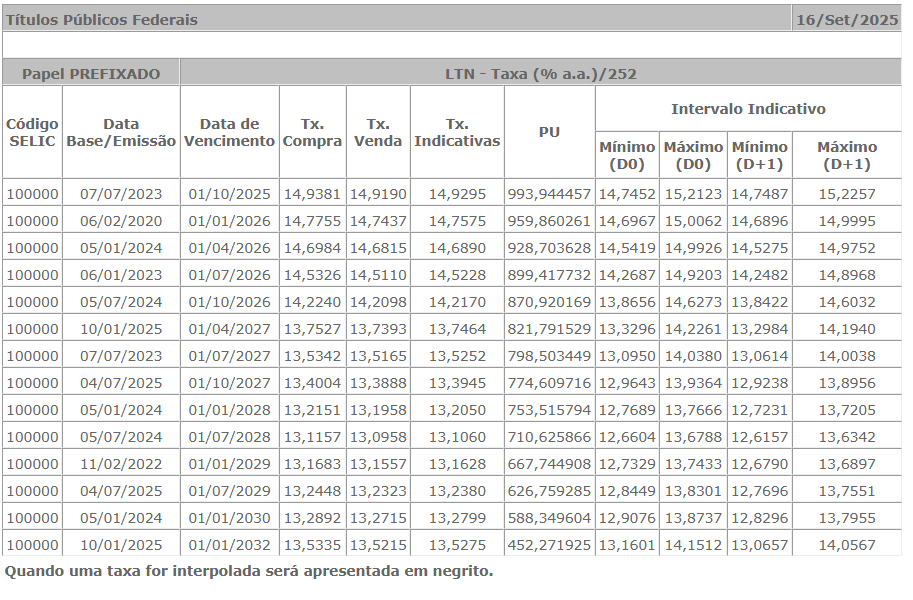
\includegraphics[width=0.7\linewidth]{ANBIMA} 

}

\caption{Taxas e preços de títulos públicos editada pela ANBIMA.}\label{fig:ANBIMA}
\end{figure}

A taxa sem risco também é denominada de taxa básica. É necessário
fazer-se o ajuste da Equação 2 para expurgar a inflação desta taxa.

\begin{equation}
\text{TMA}_{\text{ajust. sem. infl.}} = \frac{1+\text{TMA}_{\text{ajust}}}{1+\text{infl.}}-1
\end{equation}

A taxa de inflação considerada foi a mediana da expectativa do Índice de
Preços ao Consumidor Amplo (IPCA), taxa oficial de medição da inflação
brasileira, para um horizonte de 5 anos. Esta expectativa, na data de
confecção deste laudo, é de 3,90\% a.a.

Analisando-se as incertezas relacionadas à conjuntura econômica e a
condição de risco do empreendimento em análise, considerou-se um prêmio
de risco de 35\% da taxa básica adotada.

A Tabela 7 mostra as taxas consideradas e o resultado do cálculo da TMA
ajustada ao risco, com expurgo da inflação.

\begin{longtable}[]{@{}cr@{}}
\caption{Taxas consideradas para o cálculo da TMA.}\tabularnewline
\toprule\noalign{}
DESCRIÇÃO & TAXA \\
\midrule\noalign{}
\endfirsthead
\toprule\noalign{}
DESCRIÇÃO & TAXA \\
\midrule\noalign{}
\endhead
\bottomrule\noalign{}
\endlastfoot
Taxa básica (a.a.) & 13,28\% \\
Taxa básica (a.m.) & 1,04\% \\
IPCA (a.a.) & 3,90\% \\
IPCA (a.m.) & 0,32\% \\
Taxa de desconto sem infl. e sem risco (a.a.) & 9,03\% \\
Taxa de desconto sem infl. e sem risco (a.m.) & 0,72\% \\
Prêmio de risco (\% da taxa básica) & 35,00\% \\
Taxa com inflação, com risco (a.a.) & 18,55\% \\
Taxa sem inflação, com risco (a.a.) & 14,10\% \\
Taxa sem inflação, com risco (a.m.) & 1,10\% \\
\end{longtable}

Conforme apresentado na Tabela 7, a taxa mínima de atratividade ajustada
ao risco e expurgada da inflação é de 1,10\% a.m.

\subsection{Fluxo de Caixa}\label{fluxo-de-caixa}

O fluxo de caixa (FC), elaborado conforme as premissas acima, é mostrado
no \hyperref[anexo-iii]{ANEXO III}. O FC foi construído em moeda
constante, valores de set/2025.

A Tabela \ref{tab:RD} detalha as receitas e as despesas, período a
período.

A Tabela \ref{tab:FCL} apresenta o fluxo de caixa líquido do
empreendimento.

O Valor Presente Líquido (VPL) deste fluxo de caixa representa o valor
do terreno, antes do desconto de despesas iniciais utilizadas para a
aquisição da gleba, projetos, demolições, e outros. O desembolso destas
despesas ocorre, em geral, antes do início da execução física do
projeto. Estas despesas serão apresentadas e comentadas na próxima
seção.

O Valor Presente Líquido (VPL) do fluxo de caixa do empreendimento,
descontadas as despesas iniciais da Tabela 8, é de R\$ 161.199.237,50.

\subsection{Outras Despesas}\label{outras-despesas}

Algumas despesas iniciais adicionais também devem ser consideradas.
Despesas com o registro do loteamento e outras taxas cartoriais
eventualmente necessárias foram consideradas como incidindo sobre o
valor do terreno, da ordem de 1\%. Para as despesas com a aquisição dos
projetos do loteamento, foi considerado 2\% sobre os custos de
urbanização.

A Tabela 8 apresenta estes custos.

\begin{longtable}[]{@{}
  >{\raggedright\arraybackslash}p{(\linewidth - 6\tabcolsep) * \real{0.3636}}
  >{\raggedleft\arraybackslash}p{(\linewidth - 6\tabcolsep) * \real{0.1705}}
  >{\raggedleft\arraybackslash}p{(\linewidth - 6\tabcolsep) * \real{0.2386}}
  >{\raggedleft\arraybackslash}p{(\linewidth - 6\tabcolsep) * \real{0.2273}}@{}}
\caption{Despesas iniciais.}\tabularnewline
\toprule\noalign{}
\begin{minipage}[b]{\linewidth}\raggedright
ITEM
\end{minipage} & \begin{minipage}[b]{\linewidth}\raggedleft
TAXA
\end{minipage} & \begin{minipage}[b]{\linewidth}\raggedleft
REFERÊNCIA
\end{minipage} & \begin{minipage}[b]{\linewidth}\raggedleft
VALOR (R\$)
\end{minipage} \\
\midrule\noalign{}
\endfirsthead
\toprule\noalign{}
\begin{minipage}[b]{\linewidth}\raggedright
ITEM
\end{minipage} & \begin{minipage}[b]{\linewidth}\raggedleft
TAXA
\end{minipage} & \begin{minipage}[b]{\linewidth}\raggedleft
REFERÊNCIA
\end{minipage} & \begin{minipage}[b]{\linewidth}\raggedleft
VALOR (R\$)
\end{minipage} \\
\midrule\noalign{}
\endhead
\bottomrule\noalign{}
\endlastfoot
Despesas cartoriais & \(\approx1\%\) & 161.199.237,50 & 1.650.000,00 \\
Projeto & 2\% & 141.783.049,80 & 2.835.661,00 \\
Demolições & - & - & 100.000 \\
Total & - & - & 4.585.661,00 \\
\end{longtable}

\section{Enquadramento do Laudo}\label{enquadramento-do-laudo}

Conforme recomendado em ABNT (\citeproc{ref-NBR1465302}{2011}), o
presente trabalho enquadra-se como Grau II de fundamentação. Não há para
o método involutivo classificação quanto ao grau de precisão. A Tabela
\ref{tab:GF} mostra como o laudo se enquadra em cada item da ABNT
(\citeproc{ref-NBR1465302}{2011}).

\begin{longtable}[t]{r>{\raggedright\arraybackslash}p{2.5cm}>{\raggedright\arraybackslash}p{2.5cm}>{\raggedright\arraybackslash}p{2.5cm}>{\raggedright\arraybackslash}p{2.5cm}l}
\caption{\label{tab:GF}Graus de fundamentação para o método involutivo. 
      Fonte: adaptada de NBR 14.653-2}\\
\toprule
Item & Descrição & Grau III & Grau II & Grau I & Laudo\\
\midrule
\endfirsthead
\caption[]{Graus de fundamentação para o método involutiv \textit{(continued)}}\\
\toprule
Item & Descrição & Grau III & Grau II & Grau I & Laudo\\
\midrule
\endhead

\endfoot
\bottomrule
\endlastfoot
1 & Nível de detalhamento do projeto hipotético & Anteprojeto ou projeto básico & Estudo preliminar & Aproveitamento, ocupação e usos presumidos & II\\
2 & Preço de venda das unidades do projeto hipotético & No mínimo Grau II de fundamentação no método comparativo & Grau I de fundamentação no método comparativo & Estimativa & III\\
3 & Estimativa dos custos de produção & Grau III de fundamentação no método da quantificação do custo & Grau II de fundamentação no método da quantificação do custo & Grau I de fundamentação no método da quantificação do custo & I\\
4 & Prazos & Fundamentados com dados obtidos no mercado & Justificados & Arbitrados & II\\
5 & Taxas & Fundamentadas com dados obtidos no mercado & Justificadas & Arbitradas & II\\
\addlinespace
6 & Modelo & Dinâmico com fluxo de caixa & Dinâmico com equações pré-definidas & Estático & III\\
7 & Análise setorial e diagnóstico de mercado & De estrututura, conjunta, tendências e conduta & Da conjuntura & Sintéticos da conjuntura & II\\
8 & Cenários & Mínimo de 3 & 2 & 1 & III\\
9 & Análises de sensibilidade do modelo & Simulações com discussão do comportamento do modelo & Simulações com identificação das variáveis mais significativas & Sem simulação & III\\*
\end{longtable}

A Tabela 10 mostra o enquadramento para obtenção do grau de
fundamentação atingido na presente avaliação.

\begin{longtable}[]{@{}
  >{\raggedright\arraybackslash}p{(\linewidth - 6\tabcolsep) * \real{0.3071}}
  >{\centering\arraybackslash}p{(\linewidth - 6\tabcolsep) * \real{0.3286}}
  >{\centering\arraybackslash}p{(\linewidth - 6\tabcolsep) * \real{0.1571}}
  >{\centering\arraybackslash}p{(\linewidth - 6\tabcolsep) * \real{0.2071}}@{}}
\caption{Enquadramento do presente laudo.}\tabularnewline
\toprule\noalign{}
\begin{minipage}[b]{\linewidth}\raggedright
Graus
\end{minipage} & \begin{minipage}[b]{\linewidth}\centering
III
\end{minipage} & \begin{minipage}[b]{\linewidth}\centering
II
\end{minipage} & \begin{minipage}[b]{\linewidth}\centering
I
\end{minipage} \\
\midrule\noalign{}
\endfirsthead
\toprule\noalign{}
\begin{minipage}[b]{\linewidth}\raggedright
Graus
\end{minipage} & \begin{minipage}[b]{\linewidth}\centering
III
\end{minipage} & \begin{minipage}[b]{\linewidth}\centering
II
\end{minipage} & \begin{minipage}[b]{\linewidth}\centering
I
\end{minipage} \\
\midrule\noalign{}
\endhead
\bottomrule\noalign{}
\endlastfoot
Pontos Mínimos & 22 & 13 & 9 \\
Pontos Obtidos & 21 & - & - \\
Itens Obrigatórios no grau correspondente & 2,6,7 e 8, com demais no
mínimo no grau II & 2,6,7 e 8 no grau II & Todos, no mínimo, no grau
I \\
\end{longtable}

Dado que não foram atingidos os 22 pontos necessários ao enquadramento
no Grau III de Fundamentação, e o item 7 não se enquadrou no grau III ,
o laudo atingiu apenas o Grau II de fundamentação.

\section{Determinação do valor mais
provável}\label{determinauxe7uxe3o-do-valor-mais-provuxe1vel}

Temos como valor de mercado mais provável do imóvel total (gleba),
considerando o arredondamento admissível pela Norma
(\citeproc{ref-NBR1465301}{ABNT, 2019}, item 7.7.1, alínea a.), a
quantia de R\$ 161.000.000 (cento e sessenta e um milhões de reais).

No \hyperref[anexo-v]{ANEXO V} podem ser vistos os resultados da Análise
de Sensibilidade das variáveis utilizadas como \emph{input} para o
método involutivo. No \hyperref[anexo-vi]{ANEXO VI} é possível ver a
prospeção de cenários realizada para o empreendimento. Por fim, no
\hyperref[anexo-vii]{ANEXO VII} podem ser vistos os resultados de 1.000
simulações de Monte Carlo realizadas com duas distribuições \emph{a
priori} diferentes, a saber, a distribuição uniforme e a distribuição
beta. Maiores detalhes destas simulações e nossas considerações são
encontradas no próprio \hyperref[anexo-vii]{ANEXO VII}.

\section{Encerramento}\label{encerramento}

Admitimos como de boa fé e confiáveis as informações colhidas e
documentações que nos foram fornecidas, aliadas a informações colhidas
de terceiros creditados como idôneos, bem como as pesquisas realizadas e
necessárias à formação de elementos de convicção que possibilitaram a
conclusão do presente Laudo.

Os engenheiros responsáveis técnicos signatários do presente laudo se
colocam à disposição para quaisquer esclarecimentos que se fizerem
necessários.

O presente Laudo de Avaliação é composto por \pageref{LastPage} páginas,
editadas, numeradas, impressas em uma única face e rubricadas, sendo a
última assinada por seu responsável técnico e os seguintes ANEXOS:

\begin{itemize}
\tightlist
\item
  \hyperref[anexo-i]{ANEXO I} -- Avaliação do Lote Paradigma do
  Empreendimento Hipotético;
\item
  \hyperref[anexo-ii]{ANEXO II} -- Custos de Urbanização;
\item
  \hyperref[anexo-iii]{ANEXO III} -- Receitas e Despesas do
  Empreendimento.
\item
  \hyperref[anexo-iv]{ANEXO IV} -- Fluxo de Caixa Líquido do
  Empreendimento.
\item
  \hyperref[anexo-v]{ANEXO V} -- Análise de Sensibilidade
\item
  \hyperref[anexo-vi]{ANEXO VI} -- Análise de Cenários
\item
  \hyperref[anexo-vii]{ANEXO VII} -- Simulações de Monte Carlo
\item
  \hyperref[anexo-viii]{ANEXO VIII} -- Mapa da Macrozona Urbana de
  Primavera do Leste/MT
\end{itemize}

Florianópolis, \thedate

\vspace*{5\baselineskip}

\singlespacing

\noindent
\textbf{Eng.\textordmasculine\ Civil Luiz Fernando Palin Droubi}\newline
CREA Nº 5061849287-0/D-SP\newline Mestre em Engenharia de Transportes e
Gestão Territorial pela UFSC

\vspace*{5\baselineskip}

\noindent
\textbf{Eng.\textordmasculine\ Civil Lutemberg de Araújo Florencio}\newline
CREA Nº 180038699-0/D-PE\newline Doutor em Engenharia Civil pelo Núcleo
de \emph{Real Estate} da Poli/USP

\newpage

\section*{ANEXO I}\label{anexo-i}
\addcontentsline{toc}{section}{ANEXO I}

\subsection*{Avaliação do Lote Paradigma do Empreendimento
Hipotético}\label{avaliauxe7uxe3o-do-lote-paradigma-do-empreendimento-hipotuxe9tico}
\addcontentsline{toc}{subsection}{Avaliação do Lote Paradigma do
Empreendimento Hipotético}

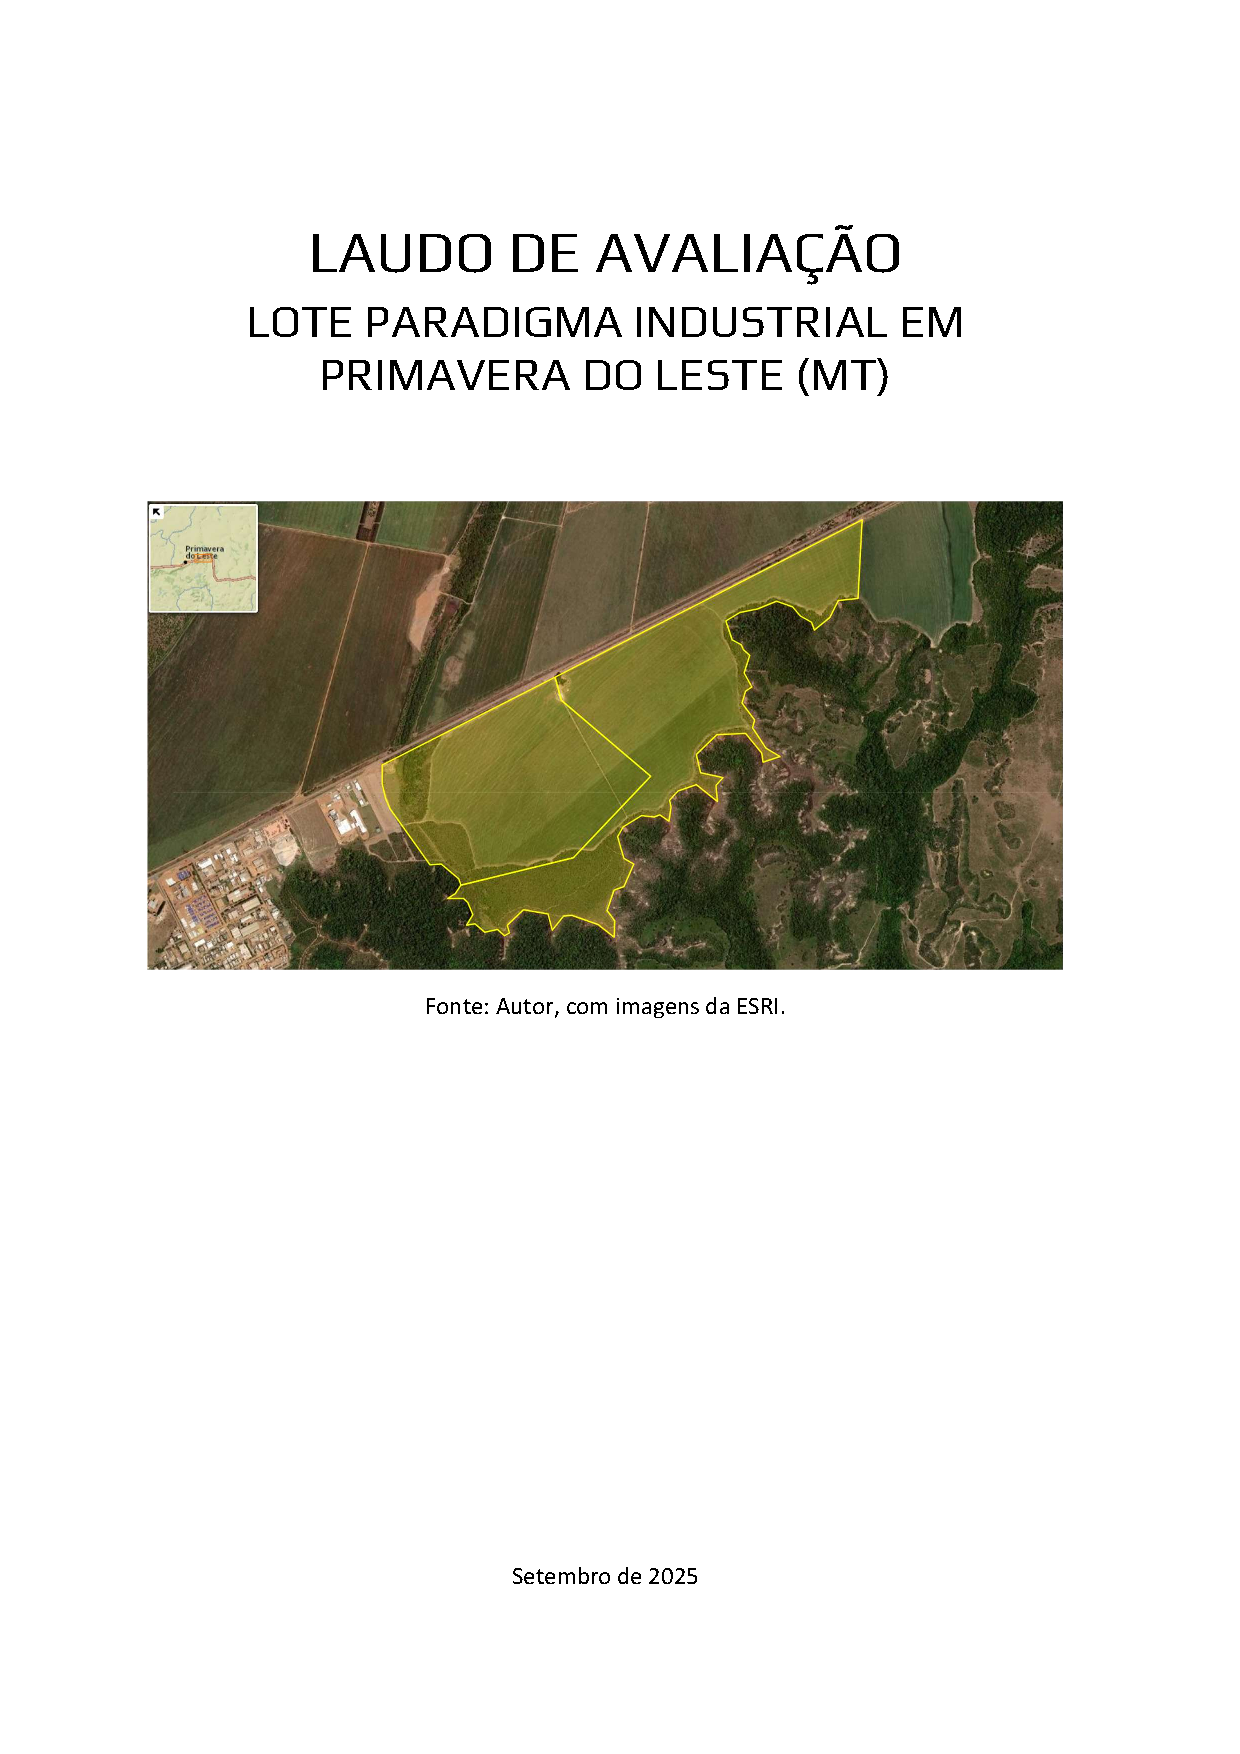
\includepdf[pages={-}]{Laudo de avaliação - Lote paradigma (VF).pdf}

\newpage

\section*{ANEXO II}\label{anexo-ii}
\addcontentsline{toc}{section}{ANEXO II}

\subsection*{Custos de Urbanização}\label{custos-de-urbanizauxe7uxe3o}
\addcontentsline{toc}{subsection}{Custos de Urbanização}

\begin{longtable}[]{@{}
  >{\raggedright\arraybackslash}p{(\linewidth - 8\tabcolsep) * \real{0.4211}}
  >{\raggedleft\arraybackslash}p{(\linewidth - 8\tabcolsep) * \real{0.1184}}
  >{\raggedleft\arraybackslash}p{(\linewidth - 8\tabcolsep) * \real{0.0526}}
  >{\raggedleft\arraybackslash}p{(\linewidth - 8\tabcolsep) * \real{0.2237}}
  >{\raggedleft\arraybackslash}p{(\linewidth - 8\tabcolsep) * \real{0.1842}}@{}}
\caption{Custos de Urbanização (R\$/1.000\(m^2\) de área
útil)*}\tabularnewline
\toprule\noalign{}
\begin{minipage}[b]{\linewidth}\raggedright
Servico
\end{minipage} & \begin{minipage}[b]{\linewidth}\raggedleft
Custo
\end{minipage} & \begin{minipage}[b]{\linewidth}\raggedleft
\%
\end{minipage} & \begin{minipage}[b]{\linewidth}\raggedleft
Valor Unitario
\end{minipage} & \begin{minipage}[b]{\linewidth}\raggedleft
Valor Total
\end{minipage} \\
\midrule\noalign{}
\endfirsthead
\toprule\noalign{}
\begin{minipage}[b]{\linewidth}\raggedright
Servico
\end{minipage} & \begin{minipage}[b]{\linewidth}\raggedleft
Custo
\end{minipage} & \begin{minipage}[b]{\linewidth}\raggedleft
\%
\end{minipage} & \begin{minipage}[b]{\linewidth}\raggedleft
Valor Unitario
\end{minipage} & \begin{minipage}[b]{\linewidth}\raggedleft
Valor Total
\end{minipage} \\
\midrule\noalign{}
\endhead
\bottomrule\noalign{}
\endlastfoot
Servicos de Topografia & 12.060 & 1 & 12 & 25.687.928 \\
Terraplenagem leve & 2.078 & 1 & 2,1 & 4.426.886 \\
Terraplenagem media & 5.968 & 0 & 0 & 0 \\
Terraplenagem pesada & 15.693 & 0 & 0 & 0 \\
Rede de Agua potavel & 11.960 & 1 & 12 & 25.473.991 \\
Rede de esgoto & 28.885 & 1 & 29 & 61.525.796 \\
Drenagem de Aguas pluviais -- galerias & 11.881 & 1 & 12 & 25.306.828 \\
Drenagem de Aguas pluviais -- guias e sarjetas & 9.787 & 1 & 9,8 &
20.846.033 \\
Pavimentacao & 31.994 & 1 & 32 & 68.147.774 \\
Rede de iluminacao publica & 3.881 & 1 & 3,9 & 8.265.635 \\
\end{longtable}

*Fonte: Editora PINI Publicação de Junho de 2025. Custos de Urbanização
calculados com base no trabalho
\say{Avaliação de Glebas –- Subsídios para Pré-Planos}

\newpage

\section*{ANEXO III}\label{anexo-iii}
\addcontentsline{toc}{section}{ANEXO III}

\subsection*{Receitas e Despesas do Empreendimento
Hipotético}\label{receitas-e-despesas-do-empreendimento-hipotuxe9tico}
\addcontentsline{toc}{subsection}{Receitas e Despesas do Empreendimento
Hipotético}

\newpage

\thispagestyle{empty}
\newgeometry{top=5mm, bottom=5mm, left=10mm, right=10mm}

\begin{landscape}\begingroup\fontsize{10}{12}\selectfont

\begin{longtable}[t]{rrrrrrrrrrrrr}
\caption{\label{tab:RD}Receitas e Despesas.}\\
\toprule
Periodo & R1 & R2 & R3 & D1 & D2 & D3 & RT & DT & RTAcum & DTAcum & Saldo & SaldoAcum\\
\midrule
\endfirsthead
\caption[]{Receitas e Despesas. \textit{(continued)}}\\
\toprule
Periodo & R1 & R2 & R3 & D1 & D2 & D3 & RT & DT & RTAcum & DTAcum & Saldo & SaldoAcum\\
\midrule
\endhead

\endfoot
\bottomrule
\endlastfoot
0 & 0 & 0 & 0 & 0 & 0 & 0 & 0 & 0 & 0 & 0 & 0 & 0\\
1 & 0 & 0 & 0 & 506.368 & 0 & 0 & 0 & 506.368 & 0 & 506.368 & -506.368 & -506.368\\
2 & 0 & 0 & 0 & 506.368 & 0 & 0 & 0 & 506.368 & 0 & 1.012.736 & -1.012.736 & -1.519.104\\
3 & 0 & 0 & 0 & 1.012.736 & 0 & 0 & 0 & 1.012.736 & 0 & 2.025.472 & -2.025.472 & -3.544.576\\
4 & 0 & 0 & 0 & 2.025.472 & 0 & 0 & 0 & 2.025.472 & 0 & 4.050.944 & -4.050.944 & -7.595.521\\
\addlinespace
5 & 0 & 0 & 0 & 3.038.208 & 0 & 0 & 0 & 3.038.208 & 0 & 7.089.152 & -7.089.152 & -14.684.673\\
6 & 0 & 0 & 0 & 3.038.208 & 0 & 0 & 0 & 3.038.208 & 0 & 10.127.361 & -10.127.361 & -24.812.034\\
7 & 0 & 0 & 0 & 3.038.208 & 0 & 0 & 0 & 3.038.208 & 0 & 13.165.569 & -13.165.569 & -37.977.603\\
8 & 0 & 0 & 0 & 3.038.208 & 0 & 0 & 0 & 3.038.208 & 0 & 16.203.777 & -16.203.777 & -54.181.380\\
9 & 0 & 0 & 0 & 4.050.944 & 0 & 0 & 0 & 4.050.944 & 0 & 20.254.721 & -20.254.721 & -74.436.101\\
\addlinespace
10 & 0 & 0 & 0 & 5.063.680 & 0 & 0 & 0 & 5.063.680 & 0 & 25.318.402 & -25.318.402 & -99.754.503\\
11 & 0 & 0 & 0 & 5.063.680 & 0 & 0 & 0 & 5.063.680 & 0 & 30.382.082 & -30.382.082 & -130.136.585\\
12 & 11.250.000 & 0 & 0 & 7.595.521 & 0 & 0 & 11.250.000 & 7.595.521 & 11.250.000 & 37.977.603 & -26.727.603 & -156.864.188\\
13 & 11.250.000 & 0 & 0 & 5.063.680 & 0 & 0 & 11.250.000 & 5.063.680 & 22.500.000 & 43.041.283 & -20.541.283 & -177.405.471\\
14 & 11.250.000 & 0 & 0 & 7.595.521 & 0 & 0 & 11.250.000 & 7.595.521 & 33.750.000 & 50.636.804 & -16.886.804 & -194.292.274\\
\addlinespace
15 & 11.250.000 & 0 & 0 & 0 & 624.521 & 0 & 11.250.000 & 624.521 & 45.000.000 & 51.261.324 & -6.261.324 & -200.553.598\\
16 & 11.250.000 & 0 & 0 & 0 & 624.521 & 0 & 11.250.000 & 624.521 & 56.250.000 & 51.885.845 & 4.364.155 & -196.189.443\\
17 & 11.250.000 & 0 & 0 & 0 & 1.249.041 & 0 & 11.250.000 & 1.249.041 & 67.500.000 & 53.134.886 & 14.365.114 & -181.824.329\\
18 & 11.250.000 & 0 & 0 & 0 & 2.498.082 & 0 & 11.250.000 & 2.498.082 & 78.750.000 & 55.632.968 & 23.117.032 & -158.707.297\\
19 & 11.250.000 & 0 & 0 & 0 & 2.498.082 & 0 & 11.250.000 & 2.498.082 & 90.000.000 & 58.131.050 & 31.868.950 & -126.838.347\\
\addlinespace
20 & 11.250.000 & 0 & 0 & 0 & 2.498.082 & 0 & 11.250.000 & 2.498.082 & 101.250.000 & 60.629.133 & 40.620.867 & -86.217.480\\
21 & 11.250.000 & 0 & 0 & 0 & 2.498.082 & 0 & 11.250.000 & 2.498.082 & 112.500.000 & 63.127.215 & 49.372.785 & -36.844.695\\
22 & 11.250.000 & 0 & 0 & 0 & 3.122.603 & 0 & 11.250.000 & 3.122.603 & 123.750.000 & 66.249.818 & 57.500.182 & 20.655.487\\
23 & 11.250.000 & 0 & 0 & 0 & 3.122.603 & 0 & 11.250.000 & 3.122.603 & 135.000.000 & 69.372.421 & 65.627.579 & 86.283.066\\
24 & 11.250.000 & 0 & 0 & 0 & 3.747.123 & 0 & 11.250.000 & 3.747.123 & 146.250.000 & 73.119.544 & 73.130.456 & 159.413.522\\
\addlinespace
25 & 11.250.000 & 0 & 0 & 0 & 3.747.123 & 0 & 11.250.000 & 3.747.123 & 157.500.000 & 76.866.668 & 80.633.332 & 240.046.854\\
26 & 11.250.000 & 0 & 0 & 0 & 4.996.165 & 0 & 11.250.000 & 4.996.165 & 168.750.000 & 81.862.832 & 86.887.168 & 326.934.022\\
27 & 11.250.000 & 0 & 0 & 0 & 6.245.206 & 0 & 11.250.000 & 6.245.206 & 180.000.000 & 88.108.038 & 91.891.962 & 418.825.984\\
28 & 7.500.000 & 3.750.000 & 0 & 0 & 9.367.809 & 0 & 11.250.000 & 9.367.809 & 191.250.000 & 97.475.847 & 93.774.153 & 512.600.137\\
29 & 0 & 11.250.000 & 0 & 0 & 6.245.206 & 0 & 11.250.000 & 6.245.206 & 202.500.000 & 103.721.053 & 98.778.947 & 611.379.085\\
\addlinespace
30 & 0 & 11.250.000 & 0 & 0 & 3.122.603 & 0 & 11.250.000 & 3.122.603 & 213.750.000 & 106.843.655 & 106.906.345 & 718.285.429\\
31 & 0 & 11.250.000 & 0 & 0 & 3.122.603 & 0 & 11.250.000 & 3.122.603 & 225.000.000 & 109.966.258 & 115.033.742 & 833.319.171\\
32 & 0 & 11.250.000 & 0 & 0 & 3.122.603 & 0 & 11.250.000 & 3.122.603 & 236.250.000 & 113.088.861 & 123.161.139 & 956.480.310\\
33 & 0 & 11.250.000 & 0 & 0 & 0 & 286.942 & 11.250.000 & 286.942 & 247.500.000 & 113.375.803 & 134.124.197 & 1.090.604.507\\
34 & 0 & 11.250.000 & 0 & 0 & 0 & 286.942 & 11.250.000 & 286.942 & 258.750.000 & 113.662.745 & 145.087.255 & 1.235.691.762\\
\addlinespace
35 & 0 & 11.250.000 & 0 & 0 & 0 & 573.884 & 11.250.000 & 573.884 & 270.000.000 & 114.236.629 & 155.763.371 & 1.391.455.133\\
36 & 0 & 11.250.000 & 0 & 0 & 0 & 573.884 & 11.250.000 & 573.884 & 281.250.000 & 114.810.512 & 166.439.488 & 1.557.894.621\\
37 & 0 & 11.250.000 & 0 & 0 & 0 & 573.884 & 11.250.000 & 573.884 & 292.500.000 & 115.384.396 & 177.115.604 & 1.735.010.225\\
38 & 0 & 11.250.000 & 0 & 0 & 0 & 1.147.768 & 11.250.000 & 1.147.768 & 303.750.000 & 116.532.164 & 187.217.836 & 1.922.228.061\\
39 & 0 & 11.250.000 & 0 & 0 & 0 & 1.147.768 & 11.250.000 & 1.147.768 & 315.000.000 & 117.679.931 & 197.320.069 & 2.119.548.129\\
\addlinespace
40 & 0 & 11.250.000 & 0 & 0 & 0 & 1.147.768 & 11.250.000 & 1.147.768 & 326.250.000 & 118.827.699 & 207.422.301 & 2.326.970.431\\
41 & 0 & 11.250.000 & 0 & 0 & 0 & 1.147.768 & 11.250.000 & 1.147.768 & 337.500.000 & 119.975.466 & 217.524.534 & 2.544.494.964\\
42 & 0 & 11.250.000 & 0 & 0 & 0 & 1.721.651 & 11.250.000 & 1.721.651 & 348.750.000 & 121.697.118 & 227.052.882 & 2.771.547.846\\
43 & 0 & 11.250.000 & 0 & 0 & 0 & 1.721.651 & 11.250.000 & 1.721.651 & 360.000.000 & 123.418.769 & 236.581.231 & 3.008.129.077\\
44 & 0 & 11.250.000 & 0 & 0 & 0 & 1.721.651 & 11.250.000 & 1.721.651 & 371.250.000 & 125.140.420 & 246.109.580 & 3.254.238.657\\
\addlinespace
45 & 0 & 3.750.000 & 7.500.000 & 0 & 0 & 2.295.535 & 11.250.000 & 2.295.535 & 382.500.000 & 127.435.955 & 255.064.045 & 3.509.302.701\\
46 & 0 & 0 & 11.250.000 & 0 & 0 & 2.295.535 & 11.250.000 & 2.295.535 & 393.750.000 & 129.731.491 & 264.018.509 & 3.773.321.211\\
47 & 0 & 0 & 11.250.000 & 0 & 0 & 2.295.535 & 11.250.000 & 2.295.535 & 405.000.000 & 132.027.026 & 272.972.974 & 4.046.294.185\\
48 & 0 & 0 & 11.250.000 & 0 & 0 & 1.721.651 & 11.250.000 & 1.721.651 & 416.250.000 & 133.748.677 & 282.501.323 & 4.328.795.508\\
49 & 0 & 0 & 11.250.000 & 0 & 0 & 2.295.535 & 11.250.000 & 2.295.535 & 427.500.000 & 136.044.212 & 291.455.788 & 4.620.251.296\\
\addlinespace
50 & 0 & 0 & 11.250.000 & 0 & 0 & 1.434.709 & 11.250.000 & 1.434.709 & 438.750.000 & 137.478.922 & 301.271.078 & 4.921.522.375\\
51 & 0 & 0 & 11.250.000 & 0 & 0 & 860.826 & 11.250.000 & 860.826 & 450.000.000 & 138.339.747 & 311.660.253 & 5.233.182.628\\
52 & 0 & 0 & 11.250.000 & 0 & 0 & 573.884 & 11.250.000 & 573.884 & 461.250.000 & 138.913.631 & 322.336.369 & 5.555.518.997\\
53 & 0 & 0 & 11.250.000 & 0 & 0 & 573.884 & 11.250.000 & 573.884 & 472.500.000 & 139.487.515 & 333.012.485 & 5.888.531.482\\
54 & 0 & 0 & 11.250.000 & 0 & 0 & 573.884 & 11.250.000 & 573.884 & 483.750.000 & 140.061.398 & 343.688.602 & 6.232.220.083\\
\addlinespace
55 & 0 & 0 & 11.250.000 & 0 & 0 & 573.884 & 11.250.000 & 573.884 & 495.000.000 & 140.635.282 & 354.364.718 & 6.586.584.801\\
56 & 0 & 0 & 11.250.000 & 0 & 0 & 573.884 & 11.250.000 & 573.884 & 506.250.000 & 141.209.166 & 365.040.834 & 6.951.625.635\\
57 & 0 & 0 & 11.250.000 & 0 & 0 & 286.942 & 11.250.000 & 286.942 & 517.500.000 & 141.496.108 & 376.003.892 & 7.327.629.527\\
58 & 0 & 0 & 11.250.000 & 0 & 0 & 286.942 & 11.250.000 & 286.942 & 528.750.000 & 141.783.050 & 386.966.950 & 7.714.596.477\\
59 & 0 & 0 & 3.750.000 & 0 & 0 & 0 & 3.750.000 & 0 & 532.500.000 & 141.783.050 & 390.716.950 & 8.105.313.428\\*
\end{longtable}
\endgroup{}
\end{landscape}

\restoregeometry

\section*{ANEXO IV}\label{anexo-iv}
\addcontentsline{toc}{section}{ANEXO IV}

\subsection*{Fluxo de Caixa do Empreendimento
Hipotético}\label{fluxo-de-caixa-do-empreendimento-hipotuxe9tico}
\addcontentsline{toc}{subsection}{Fluxo de Caixa do Empreendimento
Hipotético}

Com as receitas e despesas constantes da Tabela \ref{tab:RD}, foi
calculado o Fluxo de Caixa Líquido do empreendimento, considerando-se
para tanto um desconto nas receitas brutas de 17,62\%, referente ao BDI
do Loteador, e um acréscimo nas Despesas Brutas de 23,09\%, referente ao
BDI do Urbanizador. A Receita Líquida (RL) e a Despesa Líquida (DL)
podem ser vistas na Tabela \ref{tab:FCL}, assim como o Saldo Líquido
(SL) do caixa do empreendimento.

\begin{longtable}[t]{rrrr}
\caption{\label{tab:FCL}Fluxo de Caixa Líquido}\\
\toprule
Periodo & RL & DL & SL\\
\midrule
0 & 0 & 0,0 & 0,00\\
1 & 0 & 623.288,4 & -623.288,41\\
2 & 0 & 623.288,4 & -623.288,41\\
3 & 0 & 1.246.576,8 & -1.246.576,83\\
4 & 0 & 2.493.153,7 & -2.493.153,66\\
\addlinespace
5 & 0 & 3.739.730,5 & -3.739.730,49\\
6 & 0 & 3.739.730,5 & -3.739.730,49\\
7 & 0 & 3.739.730,5 & -3.739.730,49\\
8 & 0 & 3.739.730,5 & -3.739.730,49\\
9 & 0 & 4.986.307,3 & -4.986.307,31\\
\addlinespace
10 & 0 & 6.232.884,1 & -6.232.884,14\\
11 & 0 & 6.232.884,1 & -6.232.884,14\\
12 & 9.267.750 & 9.349.326,2 & -81.576,21\\
13 & 9.267.750 & 6.232.884,1 & 3.034.865,86\\
14 & 9.267.750 & 9.349.326,2 & -81.576,21\\
\addlinespace
15 & 9.267.750 & 768.722,4 & 8.499.027,62\\
16 & 9.267.750 & 768.722,4 & 8.499.027,62\\
17 & 9.267.750 & 1.537.444,8 & 7.730.305,24\\
18 & 9.267.750 & 3.074.889,5 & 6.192.860,49\\
19 & 9.267.750 & 3.074.889,5 & 6.192.860,49\\
\addlinespace
20 & 9.267.750 & 3.074.889,5 & 6.192.860,49\\
21 & 9.267.750 & 3.074.889,5 & 6.192.860,49\\
22 & 9.267.750 & 3.843.611,9 & 5.424.138,11\\
23 & 9.267.750 & 3.843.611,9 & 5.424.138,11\\
24 & 9.267.750 & 4.612.334,3 & 4.655.415,73\\
\addlinespace
25 & 9.267.750 & 4.612.334,3 & 4.655.415,73\\
26 & 9.267.750 & 6.149.779,0 & 3.117.970,98\\
27 & 9.267.750 & 7.687.223,8 & 1.580.526,22\\
28 & 9.267.750 & 11.530.835,7 & -2.263.085,66\\
29 & 9.267.750 & 7.687.223,8 & 1.580.526,22\\
\addlinespace
30 & 9.267.750 & 3.843.611,9 & 5.424.138,11\\
31 & 9.267.750 & 3.843.611,9 & 5.424.138,11\\
32 & 9.267.750 & 3.843.611,9 & 5.424.138,11\\
33 & 9.267.750 & 353.196,8 & 8.914.553,23\\
34 & 9.267.750 & 353.196,8 & 8.914.553,23\\
\addlinespace
35 & 9.267.750 & 706.393,5 & 8.561.356,46\\
36 & 9.267.750 & 706.393,5 & 8.561.356,46\\
37 & 9.267.750 & 706.393,5 & 8.561.356,46\\
38 & 9.267.750 & 1.412.787,1 & 7.854.962,93\\
39 & 9.267.750 & 1.412.787,1 & 7.854.962,93\\
\addlinespace
40 & 9.267.750 & 1.412.787,1 & 7.854.962,93\\
41 & 9.267.750 & 1.412.787,1 & 7.854.962,93\\
42 & 9.267.750 & 2.119.180,6 & 7.148.569,39\\
43 & 9.267.750 & 2.119.180,6 & 7.148.569,39\\
44 & 9.267.750 & 2.119.180,6 & 7.148.569,39\\
\addlinespace
45 & 9.267.750 & 2.825.574,1 & 6.442.175,86\\
46 & 9.267.750 & 2.825.574,1 & 6.442.175,86\\
47 & 9.267.750 & 2.825.574,1 & 6.442.175,86\\
48 & 9.267.750 & 2.119.180,6 & 7.148.569,39\\
49 & 9.267.750 & 2.825.574,1 & 6.442.175,86\\
\addlinespace
50 & 9.267.750 & 1.765.983,8 & 7.501.766,16\\
51 & 9.267.750 & 1.059.590,3 & 8.208.159,70\\
52 & 9.267.750 & 706.393,5 & 8.561.356,46\\
53 & 9.267.750 & 706.393,5 & 8.561.356,46\\
54 & 9.267.750 & 706.393,5 & 8.561.356,46\\
\addlinespace
55 & 9.267.750 & 706.393,5 & 8.561.356,46\\
56 & 9.267.750 & 706.393,5 & 8.561.356,46\\
57 & 9.267.750 & 353.196,8 & 8.914.553,23\\
58 & 9.267.750 & 353.196,8 & 8.914.553,23\\
59 & 3.089.250 & 0,0 & 3.089.250,00\\
\bottomrule
\end{longtable}

\subsection{Valor Presente Líquido}\label{valor-presente-luxedquido}

Dado o Fluxo de Caixa Líquido da Tabela \ref{tab:FCL}, com uma taxa de
desconto de 1,10\% a.m., chega-se a um Valor Presente Líquido de R\$
165.784.898,48. Descontando-se as despesas iniciais com taxas
cartoriais, projetos e demolições, que somam R\$ 4.585.661,00,
calcula-se um Valor Presente Líquido para o empreendimento de R\$
161.199.237,48.

\newpage

\section*{ANEXO V}\label{anexo-v}
\addcontentsline{toc}{section}{ANEXO V}

\subsection*{Análises de
Sensibilidade}\label{anuxe1lises-de-sensibilidade}
\addcontentsline{toc}{subsection}{Análises de Sensibilidade}

\subsubsection*{Preço de Venda dos
Lotes}\label{preuxe7o-de-venda-dos-lotes}
\addcontentsline{toc}{subsubsection}{Preço de Venda dos Lotes}

Inicialmente será verificada a sensibilidade do modelo
econômico-financeiro em relação à varição da variável \emph{Preço de
Venda dos Lotes}. Será adotado um intervalo de variação de \(\pm\) 15\%
em torno do valor estimado para os lotes, de R\$ 3.750.000. Assim, o
Fluxo de Caixa do Empreendimento será refeito considerando-se o valor do
lote entre R\$ 3.187.500,00 e R\$ 4.312.500,00.

\begin{figure}[H]

{\centering \includegraphics[width=0.7\linewidth]{images/SensLote-1} 

}

\caption{Análise de Sensibilidade. Valor do Lote.}\label{fig:SensLote}
\end{figure}

\subsubsection*{Custos de
Urbanização}\label{custos-de-urbanizauxe7uxe3o-1}
\addcontentsline{toc}{subsubsection}{Custos de Urbanização}

A sensibilidade do modelo econômico-financeiro em relação à varição da
variável \emph{Custos de Urbanização} será verificada. Será adotado um
intervalo de variação de \(\pm\) 10\% em torno do custo estimado, de R\$
193.783.480,80. Como o Fluxo de Caixa do Empreendimento é dividido em
três etapas de diferentes características, a variação do custo de
urbanização será realizada aplicando-se uma variação ao custo de
urbanização por 1.000 m2 de área útil previsto em cada etapa, ou seja, a
estimativa será realizada alterando-se o valor previsto de R\$
90.978,16/1.000m2 de área útil e, posteriormente, refazendo todo o Fluxo
de Caixa, para aferir a variação no Valor Presente Líquido decorrente
destas variações.

\begin{figure}[H]

{\centering \includegraphics[width=0.7\linewidth]{images/SensCUrb-1} 

}

\caption{Análise de Sensibilidade. Custos de Urbanização.}\label{fig:SensCUrb}
\end{figure}

\subsubsection*{Taxa mínima de
atratividade}\label{taxa-muxednima-de-atratividade}
\addcontentsline{toc}{subsubsection}{Taxa mínima de atratividade}

Por fim, foi realizada a análise de sensibilidade da variável \emph{taxa
mínima de atratividade}, incluso o risco. Na prática, foi realizada a
alteração do prêmio de risco, dentro do intervalo de 20\% e 50\%, o que,
por sua vez levou a um intervalo de varição da taxa mínima de
atratividade entre

\begin{figure}[H]

{\centering \includegraphics[width=0.7\linewidth]{images/SensTMA-1} 

}

\caption{Análise de Sensibilidade. TMA (\%).}\label{fig:SensTMA}
\end{figure}

\newpage

\section*{ANEXO VI}\label{anexo-vi}
\addcontentsline{toc}{section}{ANEXO VI}

\subsection*{Cenários}\label{cenuxe1rios}
\addcontentsline{toc}{subsection}{Cenários}

O estudo de cenários também é recomendado pela ABNT
(\citeproc{ref-NBR1465302}{2011}) quando se usa o método involutivo.

Comumente, analisam-se 3 cenários: um mais provável ou neutro, um
cenário pessimista e um cenário otimista. Nestes cenários são
consideradas variações simultâneas nas variáveis chaves do fluxo de
caixa.

O cenário mais provável é aquele já apresentado para determinar o valor
da gleba.

Para os cenários pessimista e otimista consideram-se variações
simultâneas nas variáveis chaves, todas na mesma direção. Ou seja, uma
combinação de variáveis que diminuem o valor da gleba (cenário
pessimista) ou aumentam o valor dela (cenário otimista).

\subsubsection*{Cenário mais
provável}\label{cenuxe1rio-mais-provuxe1vel}
\addcontentsline{toc}{subsubsection}{Cenário mais provável}

A Tabela 14 abaixo mostra os valores considerados no cenário mais
provável.

\begin{longtable}[]{@{}
  >{\raggedright\arraybackslash}p{(\linewidth - 4\tabcolsep) * \real{0.3704}}
  >{\raggedleft\arraybackslash}p{(\linewidth - 4\tabcolsep) * \real{0.1235}}
  >{\raggedleft\arraybackslash}p{(\linewidth - 4\tabcolsep) * \real{0.5062}}@{}}
\caption{Cenário mais provável.}\tabularnewline
\toprule\noalign{}
\begin{minipage}[b]{\linewidth}\raggedright
Item
\end{minipage} & \begin{minipage}[b]{\linewidth}\raggedleft
Variação
\end{minipage} & \begin{minipage}[b]{\linewidth}\raggedleft
Valor
\end{minipage} \\
\midrule\noalign{}
\endfirsthead
\toprule\noalign{}
\begin{minipage}[b]{\linewidth}\raggedright
Item
\end{minipage} & \begin{minipage}[b]{\linewidth}\raggedleft
Variação
\end{minipage} & \begin{minipage}[b]{\linewidth}\raggedleft
Valor
\end{minipage} \\
\midrule\noalign{}
\endhead
\bottomrule\noalign{}
\endlastfoot
PU de Venda do Lote & 0,0\% & R\$ 250\(/m^2\) \\
Custos de Urbanização & 0,0\% & R\$ 112,53\(/m^2 \text{a.u.}\) \\
Adicional ao Prêmio de Risco & 0,0\% & 35\% \\
\end{longtable}

\subsubsection*{Cenário pessimista}\label{cenuxe1rio-pessimista}
\addcontentsline{toc}{subsubsection}{Cenário pessimista}

Como a combinação de todos os eventos extremos é pouco provável,
tomar-se-ão situações intermediárias. A Tabela 15 abaixo apresenta as
variações consideradas no cenário pessimista.

\begin{longtable}[]{@{}
  >{\raggedright\arraybackslash}p{(\linewidth - 4\tabcolsep) * \real{0.3409}}
  >{\raggedleft\arraybackslash}p{(\linewidth - 4\tabcolsep) * \real{0.1364}}
  >{\raggedleft\arraybackslash}p{(\linewidth - 4\tabcolsep) * \real{0.5227}}@{}}
\caption{Cenário pessimista.}\tabularnewline
\toprule\noalign{}
\begin{minipage}[b]{\linewidth}\raggedright
Item
\end{minipage} & \begin{minipage}[b]{\linewidth}\raggedleft
Variação
\end{minipage} & \begin{minipage}[b]{\linewidth}\raggedleft
Valor
\end{minipage} \\
\midrule\noalign{}
\endfirsthead
\toprule\noalign{}
\begin{minipage}[b]{\linewidth}\raggedright
Item
\end{minipage} & \begin{minipage}[b]{\linewidth}\raggedleft
Variação
\end{minipage} & \begin{minipage}[b]{\linewidth}\raggedleft
Valor
\end{minipage} \\
\midrule\noalign{}
\endhead
\bottomrule\noalign{}
\endlastfoot
PU de Venda do Lote & -0,05\% & R\$ 237,50\(/m^2\) \\
Custos de Urbanização & +0,05\% & R\$ 118,15\(/m^2 \text{a.u.}\) \\
Adicional ao Prêmio de Risco & +7,50 p.p. & 42,50\% \\
\end{longtable}

\subsubsection*{Cenário otimista}\label{cenuxe1rio-otimista}
\addcontentsline{toc}{subsubsection}{Cenário otimista}

Também neste caso, a combinação de todos os eventos extremos é pouco
provável. Tomar-se-ão, então, situações intermediárias. A Tabela 14
abaixo apresenta as variações consideradas no cenário pessimista.

\begin{longtable}[]{@{}
  >{\raggedright\arraybackslash}p{(\linewidth - 4\tabcolsep) * \real{0.3488}}
  >{\raggedleft\arraybackslash}p{(\linewidth - 4\tabcolsep) * \real{0.1395}}
  >{\raggedleft\arraybackslash}p{(\linewidth - 4\tabcolsep) * \real{0.5116}}@{}}
\caption{Cenário otimista.}\tabularnewline
\toprule\noalign{}
\begin{minipage}[b]{\linewidth}\raggedright
Item
\end{minipage} & \begin{minipage}[b]{\linewidth}\raggedleft
Variação
\end{minipage} & \begin{minipage}[b]{\linewidth}\raggedleft
Valor
\end{minipage} \\
\midrule\noalign{}
\endfirsthead
\toprule\noalign{}
\begin{minipage}[b]{\linewidth}\raggedright
Item
\end{minipage} & \begin{minipage}[b]{\linewidth}\raggedleft
Variação
\end{minipage} & \begin{minipage}[b]{\linewidth}\raggedleft
Valor
\end{minipage} \\
\midrule\noalign{}
\endhead
\bottomrule\noalign{}
\endlastfoot
Preço de Venda do Lote & +5,00\% & 262,50\(/m^2\) \\
Custos de Urbanização & -5,00\% & 106,90\(/m^2 \text{a.u.}\) \\
Adicional ao Prêmio de Risco & -7,50 p.p. & 27,5\% \\
\end{longtable}

\subsection*{Resultados}\label{resultados}
\addcontentsline{toc}{subsection}{Resultados}

A Tabela 17 mostra os resultados para os 3 cenários simulados. A Figura
\ref{fig:Cenarios} ilustra com um gráfico o impacto no valor da gleba.

\begin{longtable}[]{@{}
  >{\raggedright\arraybackslash}p{(\linewidth - 4\tabcolsep) * \real{0.3659}}
  >{\raggedleft\arraybackslash}p{(\linewidth - 4\tabcolsep) * \real{0.2683}}
  >{\raggedleft\arraybackslash}p{(\linewidth - 4\tabcolsep) * \real{0.3659}}@{}}
\caption{Cenário otimista.}\tabularnewline
\toprule\noalign{}
\begin{minipage}[b]{\linewidth}\raggedright
Cenário
\end{minipage} & \begin{minipage}[b]{\linewidth}\raggedleft
Valor da Gleba
\end{minipage} & \begin{minipage}[b]{\linewidth}\raggedleft
Variação (\%)
\end{minipage} \\
\midrule\noalign{}
\endfirsthead
\toprule\noalign{}
\begin{minipage}[b]{\linewidth}\raggedright
Cenário
\end{minipage} & \begin{minipage}[b]{\linewidth}\raggedleft
Valor da Gleba
\end{minipage} & \begin{minipage}[b]{\linewidth}\raggedleft
Variação (\%)
\end{minipage} \\
\midrule\noalign{}
\endhead
\bottomrule\noalign{}
\endlastfoot
Pessimista & R\$ 134.704.096,97 & -16,44\% \\
Provável & R\$ 161.199.237,48 & 0,0\% \\
Otimista & R\$ 189.599.304,70 & 17,62\% \\
\end{longtable}

\begin{figure}[H]

{\centering \includegraphics[width=0.7\linewidth]{images/Cenarios-1} 

}

\caption{Valor da Gleba para diferentes cenários.}\label{fig:Cenarios}
\end{figure}

\newpage

\section*{ANEXO VII}\label{anexo-vii}
\addcontentsline{toc}{section}{ANEXO VII}

\subsection*{Simulações de Monte Carlo com distribuição
uniforme}\label{simulauxe7uxf5es-de-monte-carlo-com-distribuiuxe7uxe3o-uniforme}
\addcontentsline{toc}{subsection}{Simulações de Monte Carlo com
distribuição uniforme}

Foram realizadas \(n =\) 1000 simulações de Monte Carlo considerando que
as variáveis-chave VU do Lote Paradigma (VU), Custos de Construção (CC)
e Taxa Mínima de Atratividade (TMA) variam em um determinado
\emph{range} de valores \textbf{de maneira uniforme}. Os \emph{ranges}
de valores considerados foram:

\begin{itemize}
\tightlist
\item
  VU: de 90\% a 110\% do valor da estimativa central para o lote
  paradigma;
\item
  CC: de 85\% a 115\% dos custos de urbanização descritos no
  \hyperref[anexo-ii]{ANEXO II};
\item
  TMA: de 85\% a 115\% da TMA utilizada para estimar o valor central da
  gleba (1,10\%).
\end{itemize}

Para a simulação foi adotado que a correlação entre as variáveis
segueria o exposto na Tabela \ref{tab:dependencia}.

\begin{longtable}[t]{lrrr}
\caption{\label{tab:dependencia}Matriz de Covariancia -- variaveis 50\% dependentes}\\
\toprule
 & VU & CC & TMA\\
\midrule
\cellcolor{gray!10}{VU} & \cellcolor{gray!10}{1.0} & \cellcolor{gray!10}{0.5} & \cellcolor{gray!10}{-0.5}\\
CC & 0.5 & 1.0 & 0.5\\
\cellcolor{gray!10}{TMA} & \cellcolor{gray!10}{-0.5} & \cellcolor{gray!10}{0.5} & \cellcolor{gray!10}{1.0}\\
\bottomrule
\end{longtable}

Os resultados das simulações podem ser visualizados no histograma da
Figura \ref{fig:unifMC}.

\begin{figure}[H]

{\centering \includegraphics[width=0.6\linewidth]{images/unifMC-1} 

}

\caption{Simulações de Monte Carlo com distribuição a priori uniforme.}\label{fig:unifMC}
\end{figure}

O valor médio dos VPL obtidos com as simulações foi de R\$
161.657.628,41, com desvio-padrão igual a R\$ 22.294.642,16. Apenas 10\%
dos valores ficaram abaixo de R\$ 132.554.621,49 e outros 10\% ficaram
acima de R\$ 191.561.104,79. Esta grande dispersão dos valores em torno
da média deve-se ao fato que a distribuição a priori adotada foi a
distribuição uniforme, que atribui igual probabilidade de ocorrência a
quaisquer valores dentro do \emph{range} de valores admissíveis
pré-estabelecido.

\subsection*{Simulações de Monte Carlo com distribuição
beta}\label{simulauxe7uxf5es-de-monte-carlo-com-distribuiuxe7uxe3o-beta}
\addcontentsline{toc}{subsection}{Simulações de Monte Carlo com
distribuição beta}

Nas simulações da seção anterior, a distribuição dos valores dentro do
\emph{range} de valores pré-estabelecido para cada variável foi
considerada uniforme, como antes esclarecido. No entanto, é razoável
supor que há uma maior probabilidade de ocorrência dos valores centrais
do que dos valores extremos dos intervalos de valores pré-estabelecidos.
A distribuição beta é utilizada, em geral, para simular a maior
probabilidade de ocorrência dos valores centrais, propiciando assim
simulações mais realistas. Assim, foram elaboradas \(n =\) 1000
simulações de Monte Carlo, considerando os mesmos \emph{ranges} antes
estabelecidos para as simulações com distribuição uniforme, porém agora
com distribuição de probabilidade beta com parâmetros de forma ambos
iguais a 7.

Os resultados das simulações podem ser visualizados no histograma da
Figura \ref{fig:betaMC}.

\begin{figure}[H]

{\centering \includegraphics[width=0.7\linewidth]{images/betaMC-1} 

}

\caption{Simulações de Monte Carlo com distribuição a priori beta.}\label{fig:betaMC}
\end{figure}

Baseados nas \(n =\) 1000 simulações efetuadas, obteve-se um valor médio
de \(\overline{X} = \text{R\$ }\) 161.287.587,91, com desvio-padrão
igual a \(s = \text{R\$ }\) 10.048.563,60. Com estes parâmetros foi
elaborada a Figura abaixo, em que mostra-se com a distribuição normal
teórica, 80\% dos valores ficaram dentro do intervalo laranja, entre R\$
148.409.835,49 e R\$ 174.165.340,33. Tais valores foram, após
arredondamento, utilizados para formar o \emph{intervalo de valores
prováveis}. Este intervalo foi adotado como uma espécie de intervalo de
confiança para o valor central da gleba, apesar de não haver
procedimento normatizado para este fim quando da utilização do Método
Involutivo.

\begin{figure}[H]

{\centering \includegraphics[width=0.7\linewidth]{images/unnamed-chunk-22-1} 

}

\caption{Distribuição Teórica com parâmetros estimados segundo simulações de Monte Carlo.}\label{fig:unnamed-chunk-22}
\end{figure}

Com relação às simulações, 10\% dos valores ficaram abaixo de R\$
148.373.461,60 e outros 10\% ficaram acima de R\$ 174.061.148,28,
quantis muito próximos aos obtidos com os parâmetros da distribuição
normal ajustada aos dados, o que mostra a convergência das simulações
conforme o Teorema Central do Limite.

\newpage

\section*{ANEXO VIII}\label{anexo-viii}
\addcontentsline{toc}{section}{ANEXO VIII}

\begin{landscape}

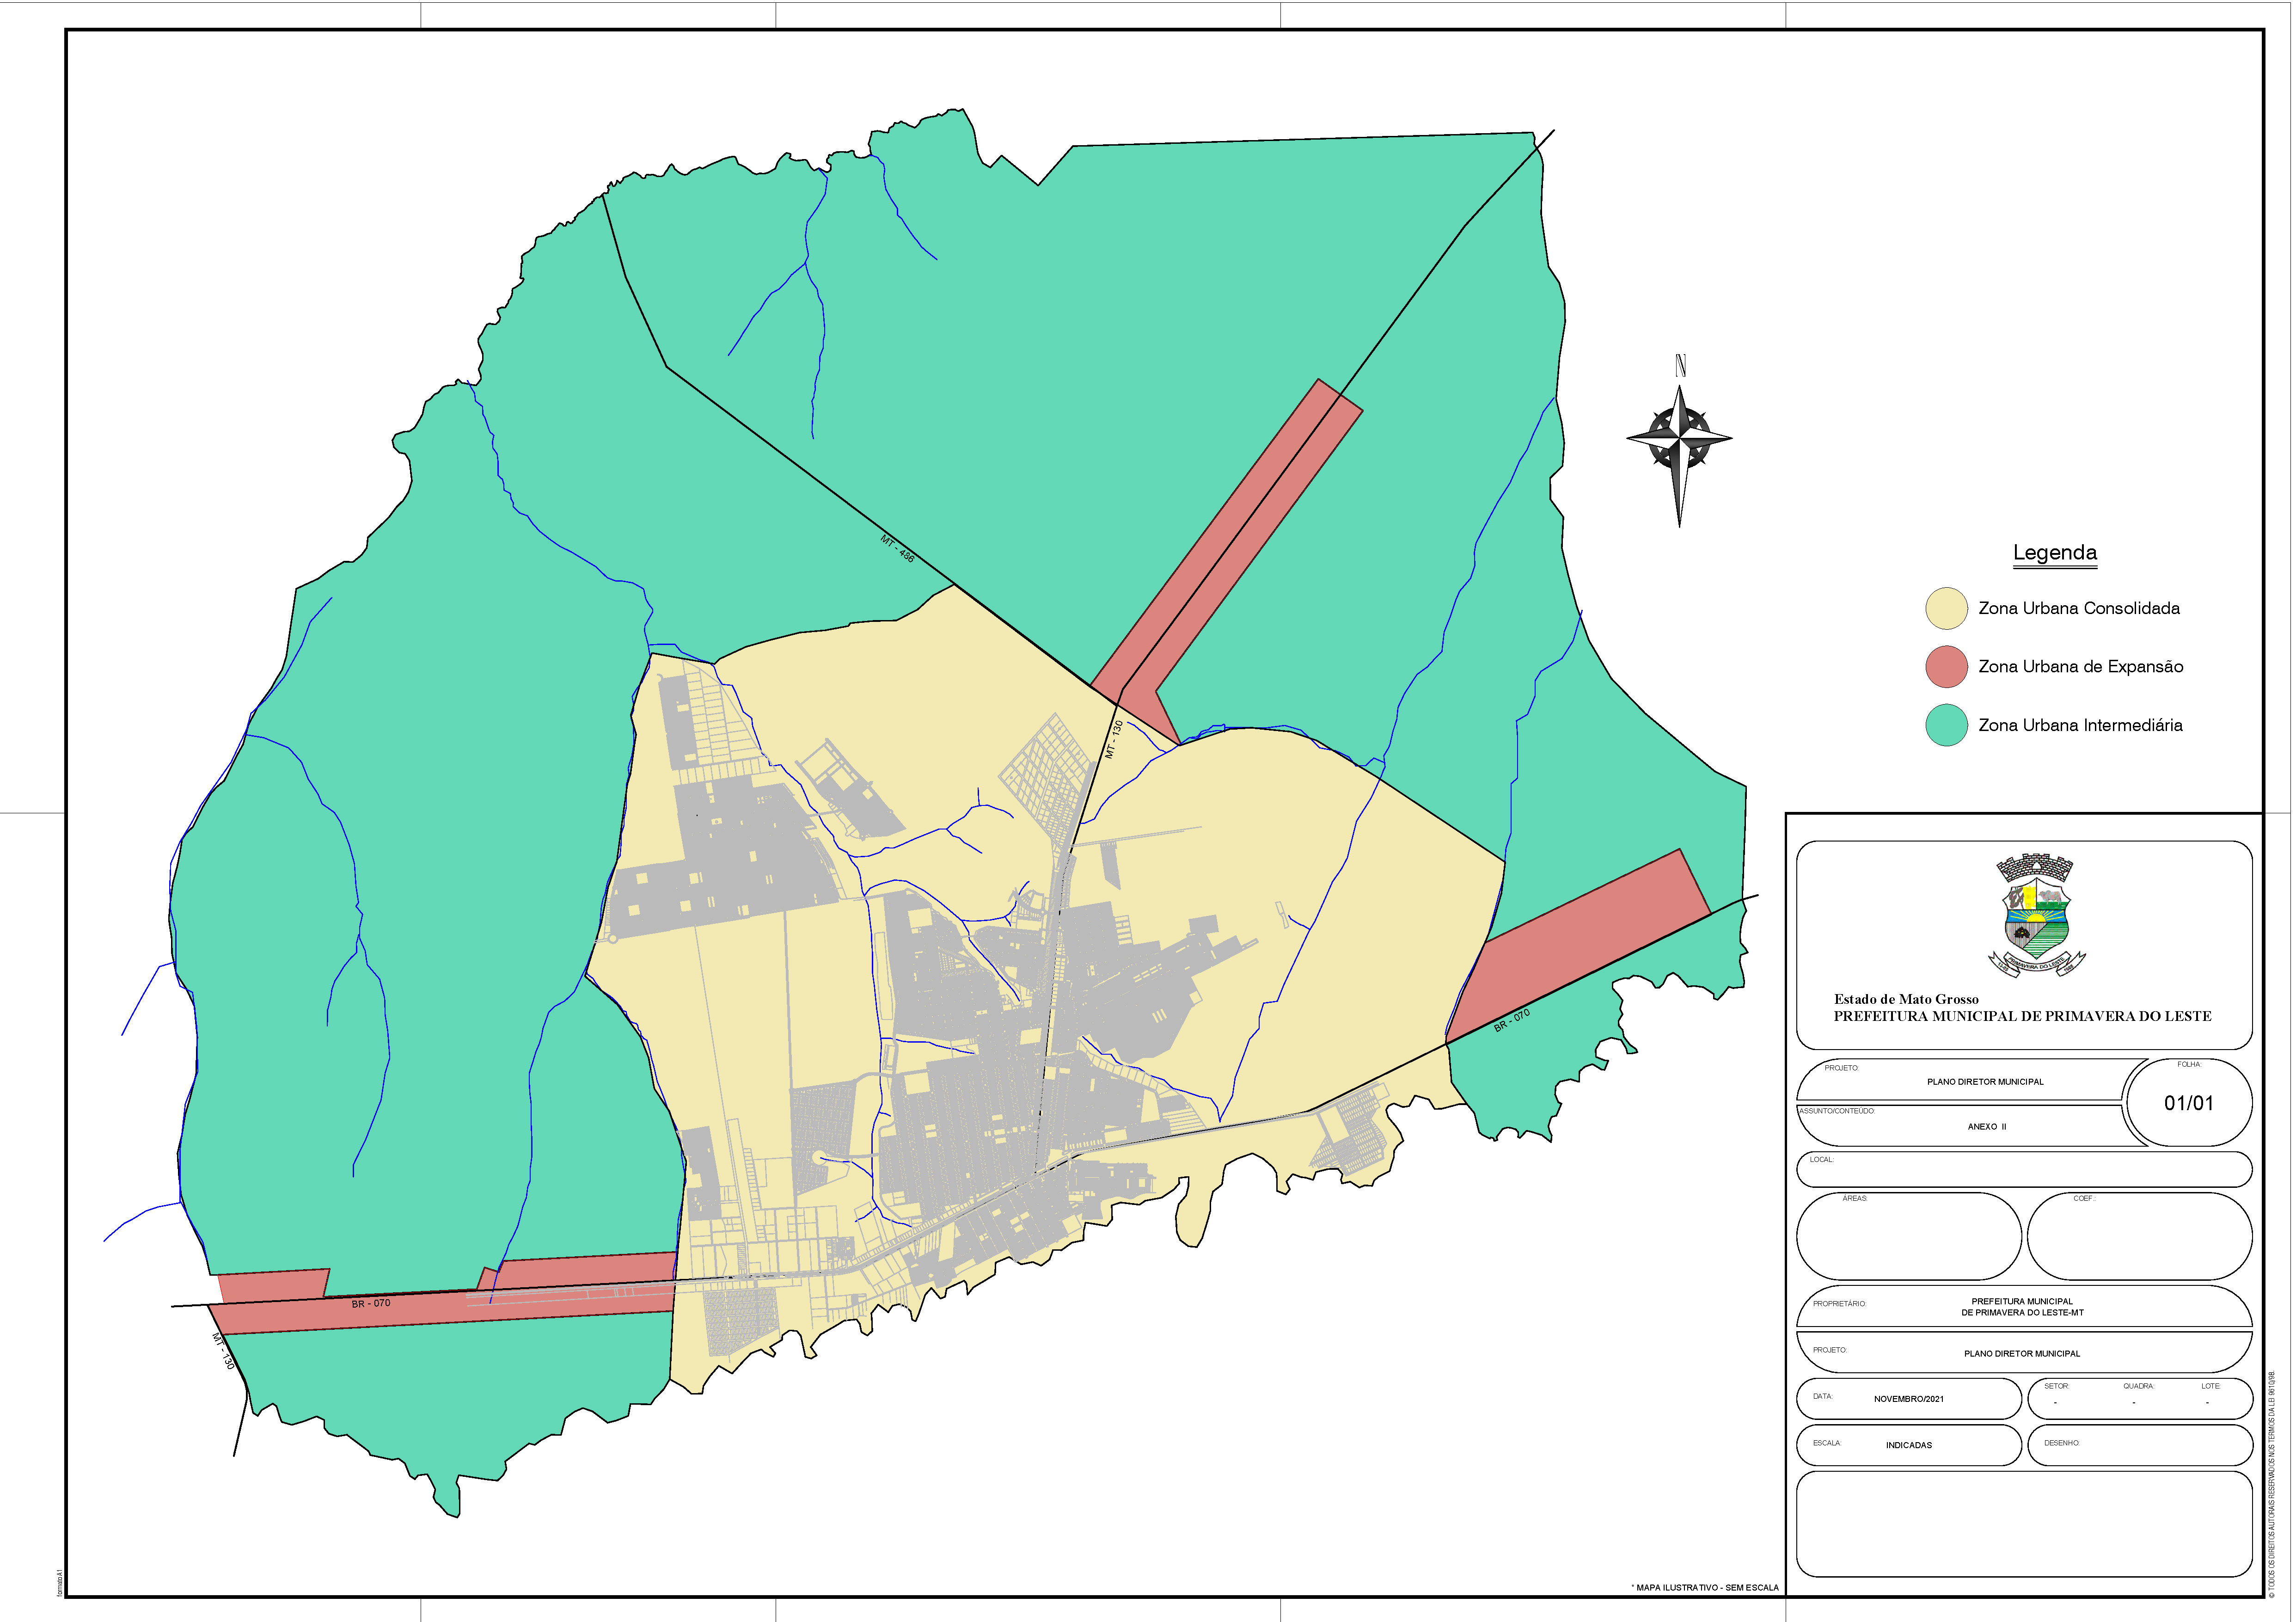
\includepdf[pages={-},angle=90]{Macrozona Urbana-R00-A1.pdf}

\end{landscape}

\section*{ANEXO IX}\label{anexo-ix}
\addcontentsline{toc}{section}{ANEXO IX}

\subsection*{Documentação
utilizada}\label{documentauxe7uxe3o-utilizada-1}
\addcontentsline{toc}{subsection}{Documentação utilizada}

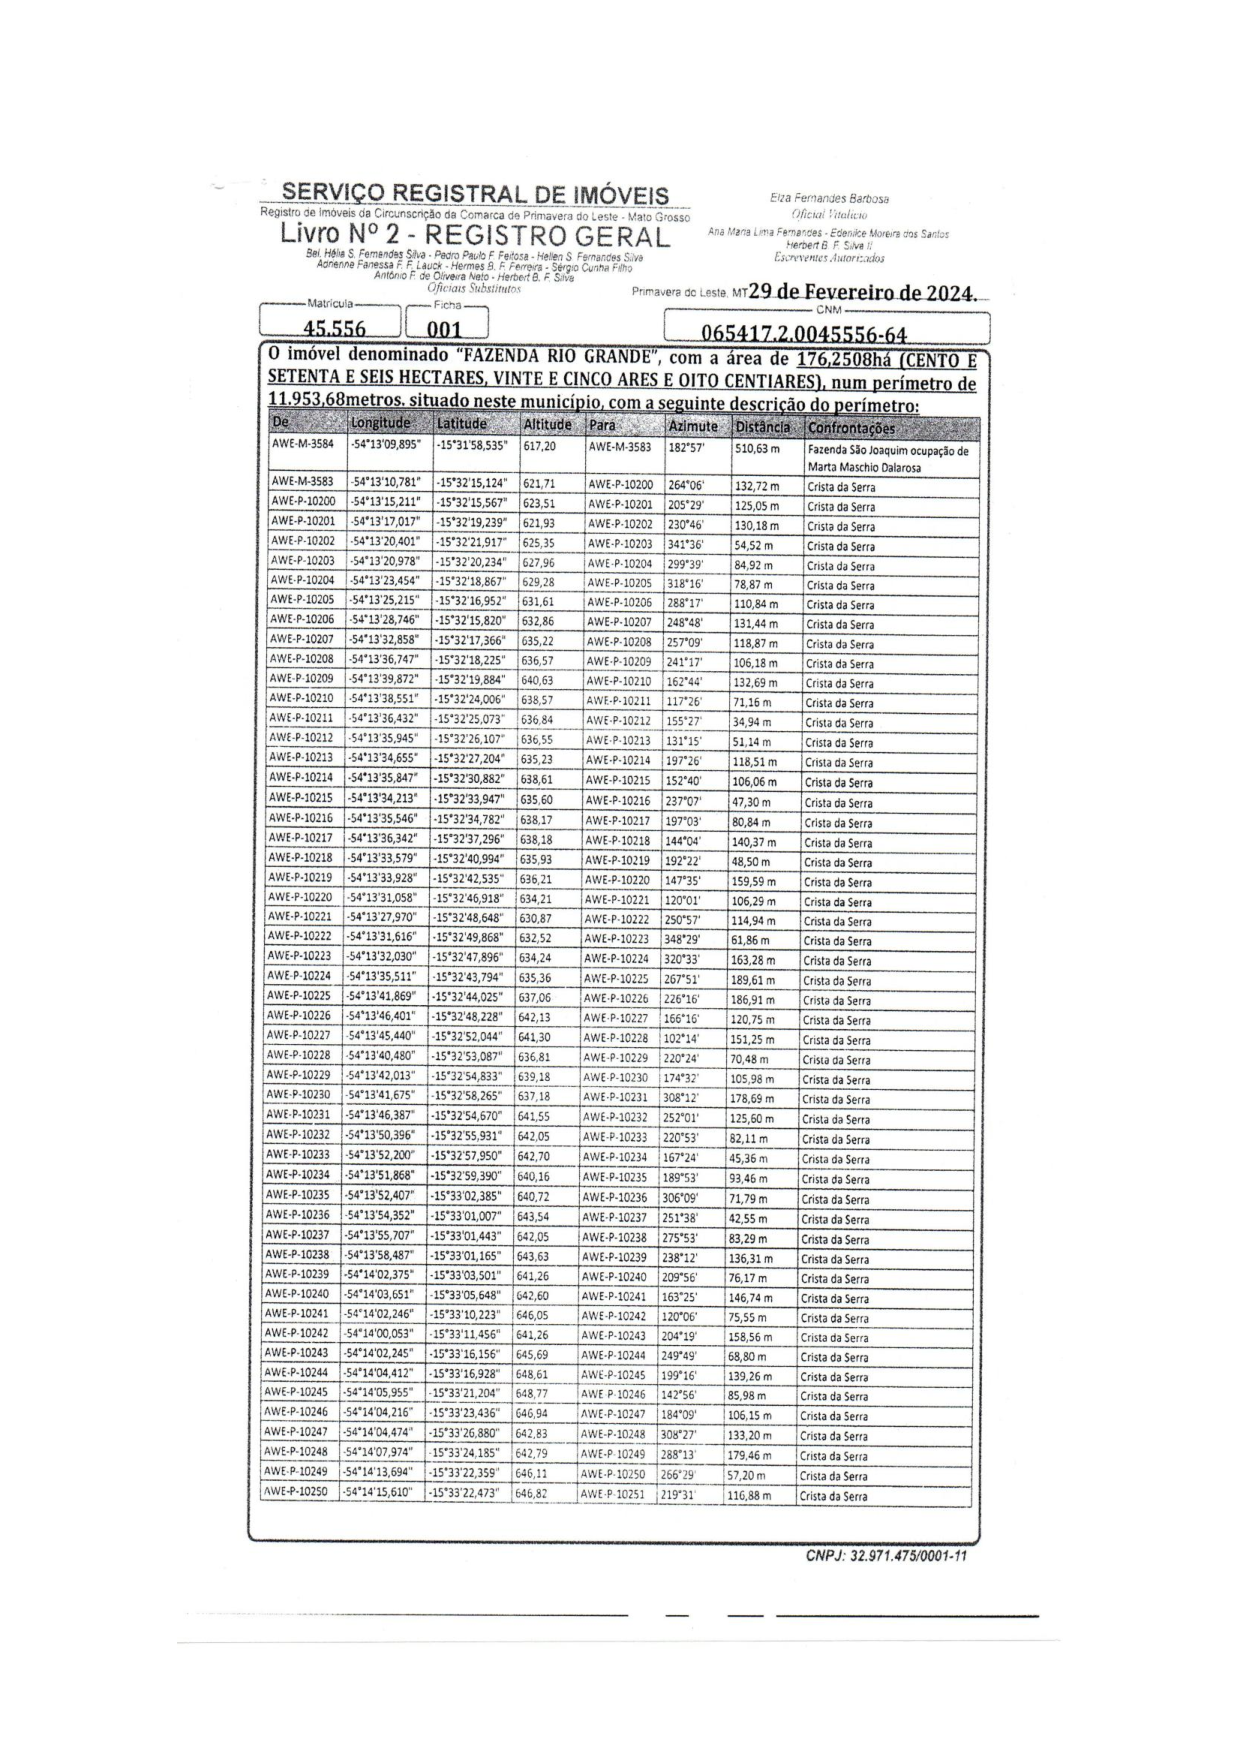
\includepdf[pages={-}]{./refs/MAT 45556_ANTONIO VARGAS.pdf}

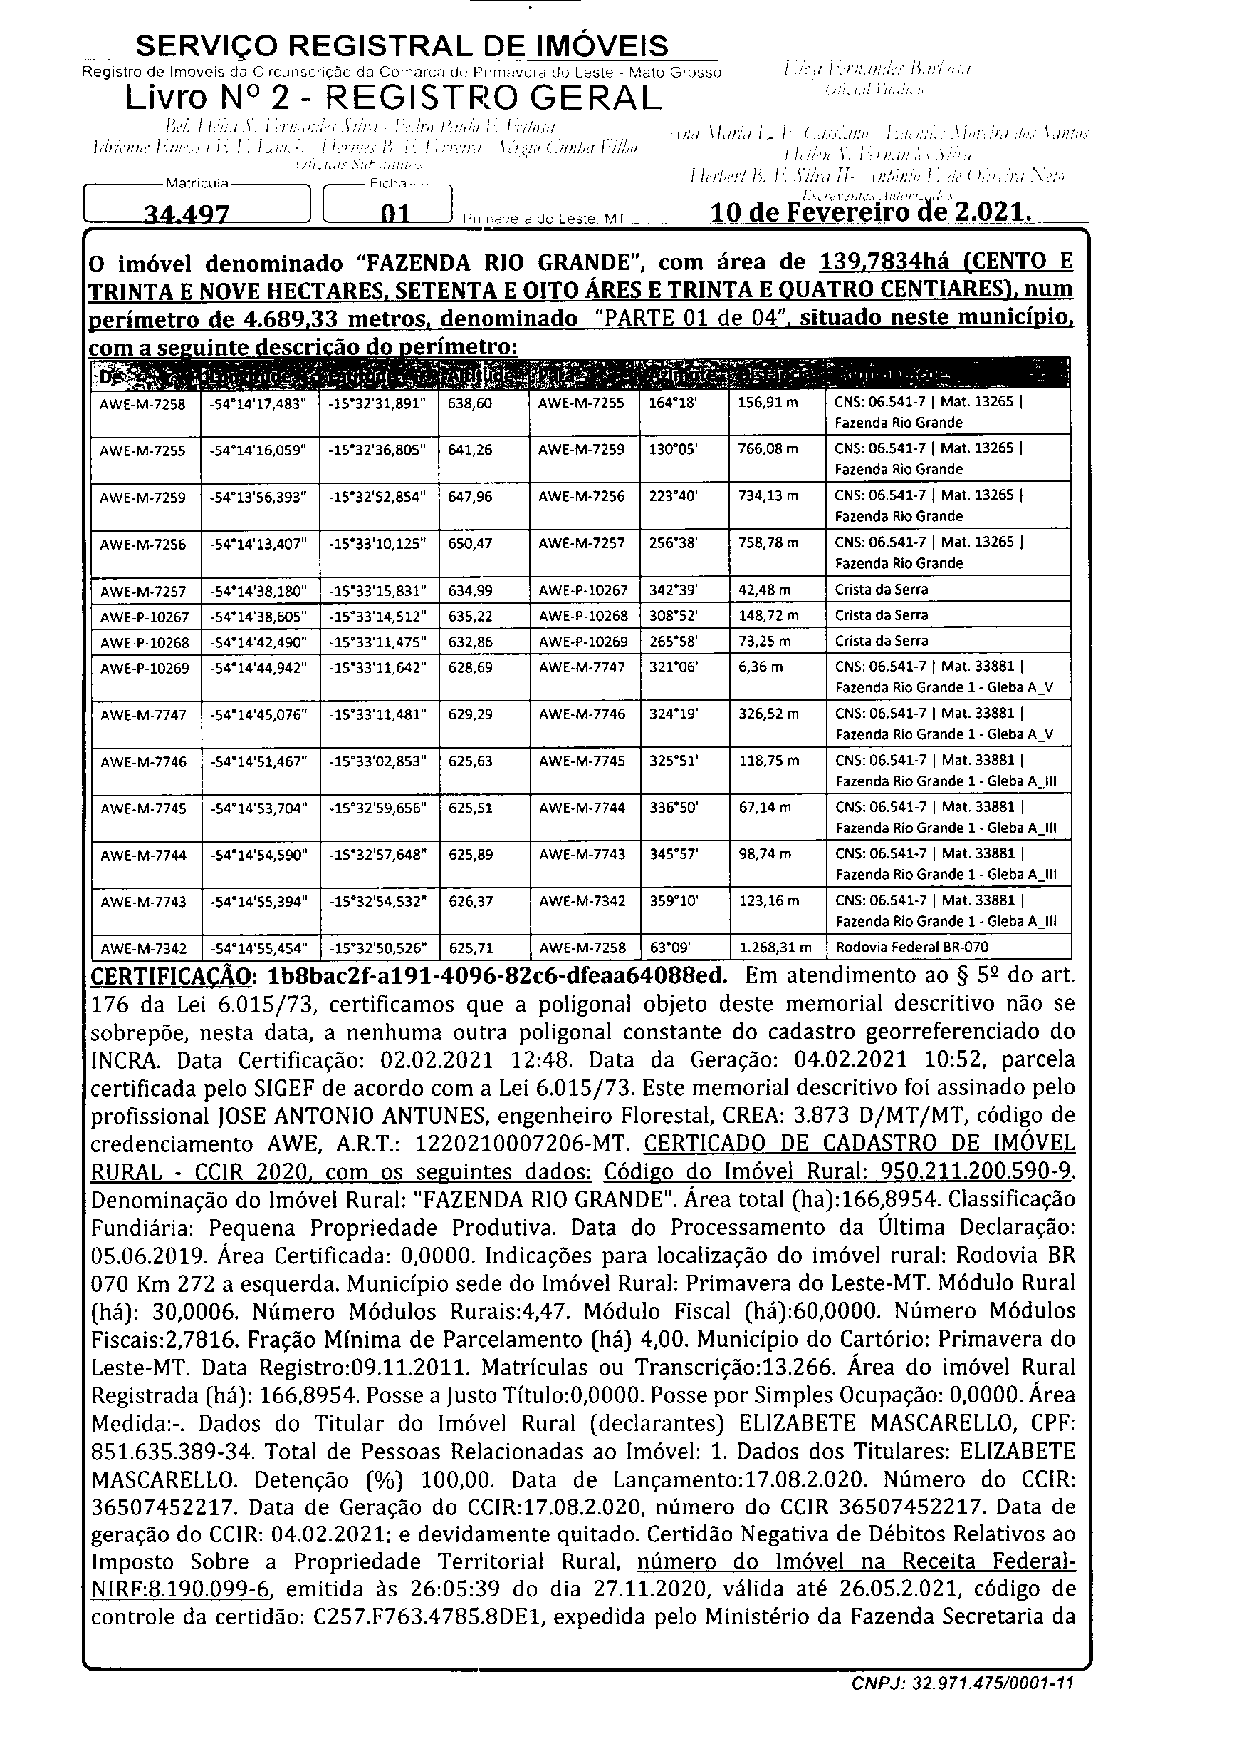
\includepdf[pages={-}]{./refs/MAT 34497_ELIZABETE MASCARELLO.pdf}

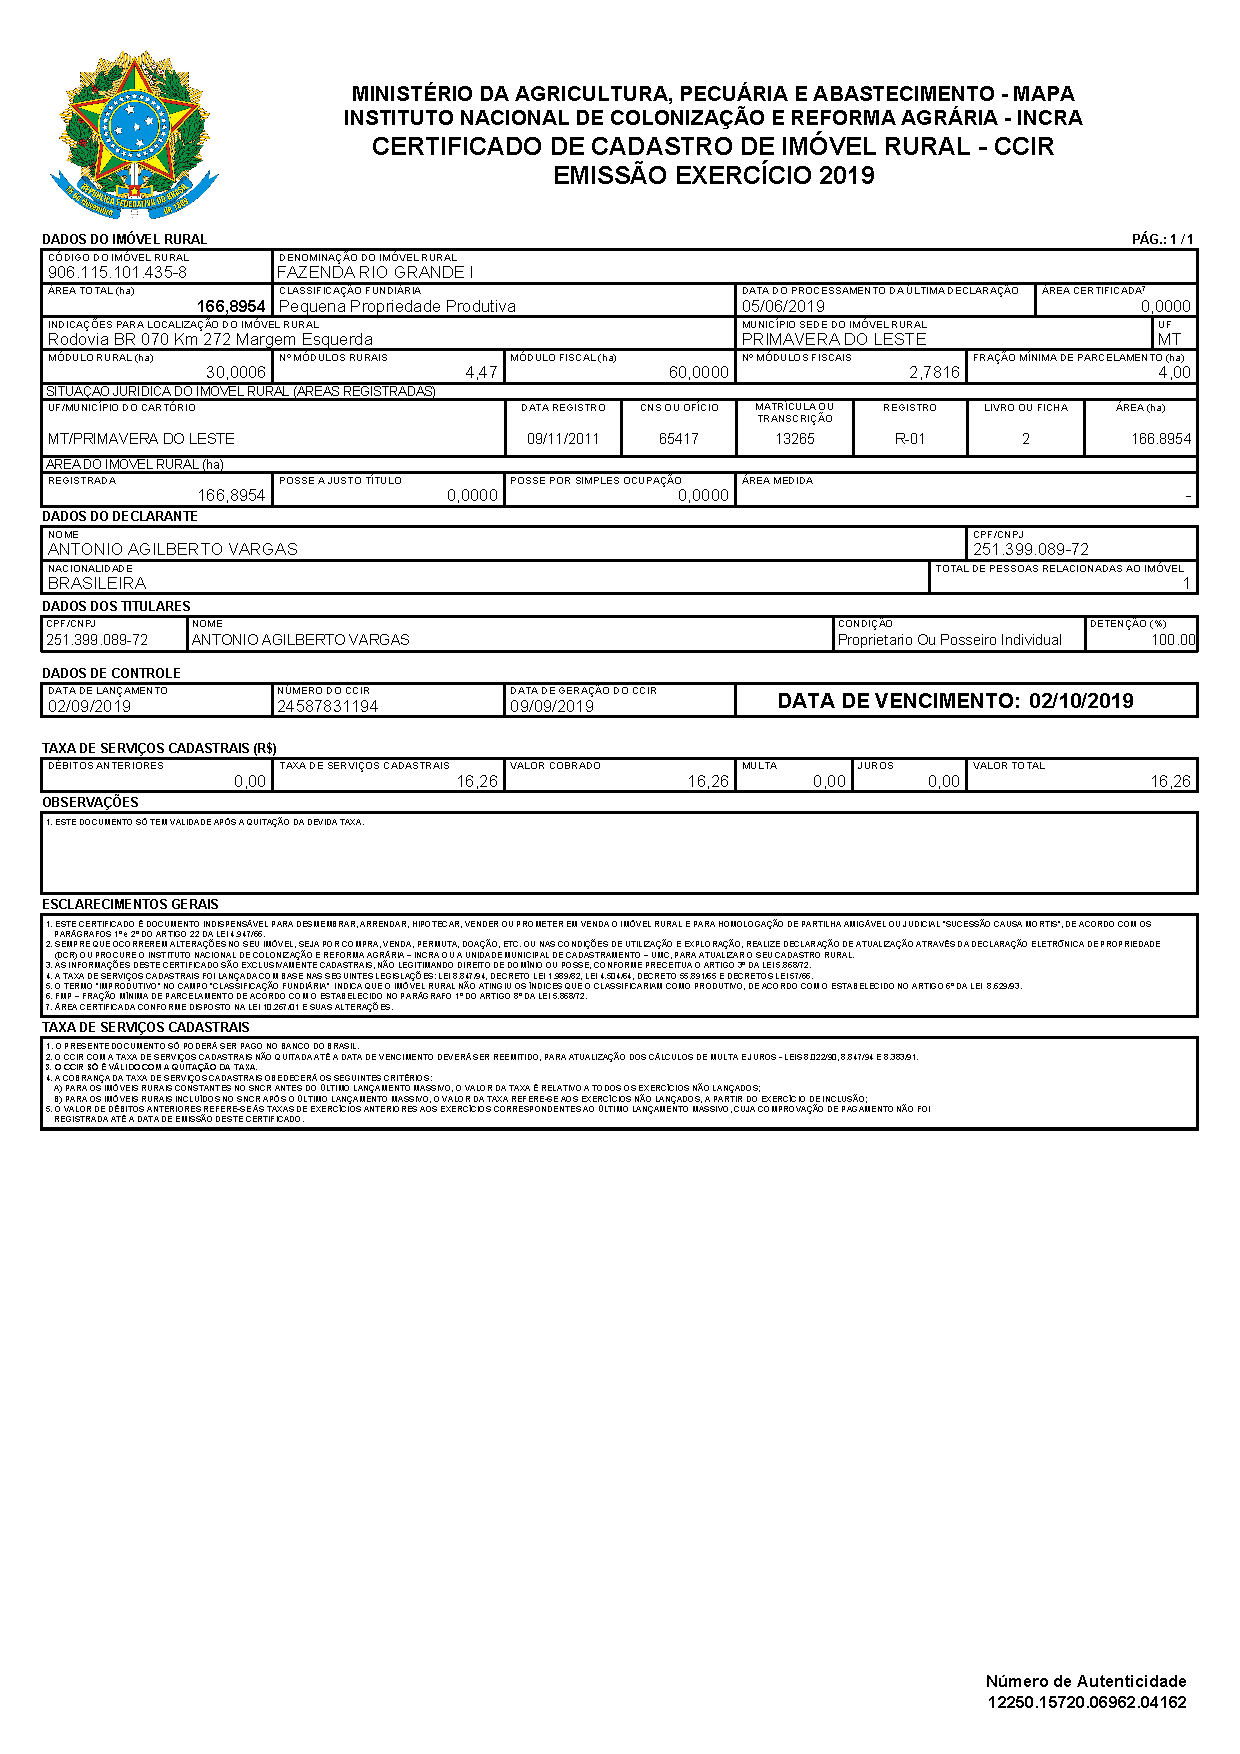
\includepdf[pages={-}]{./refs/CCIR_ANTONIO.pdf}

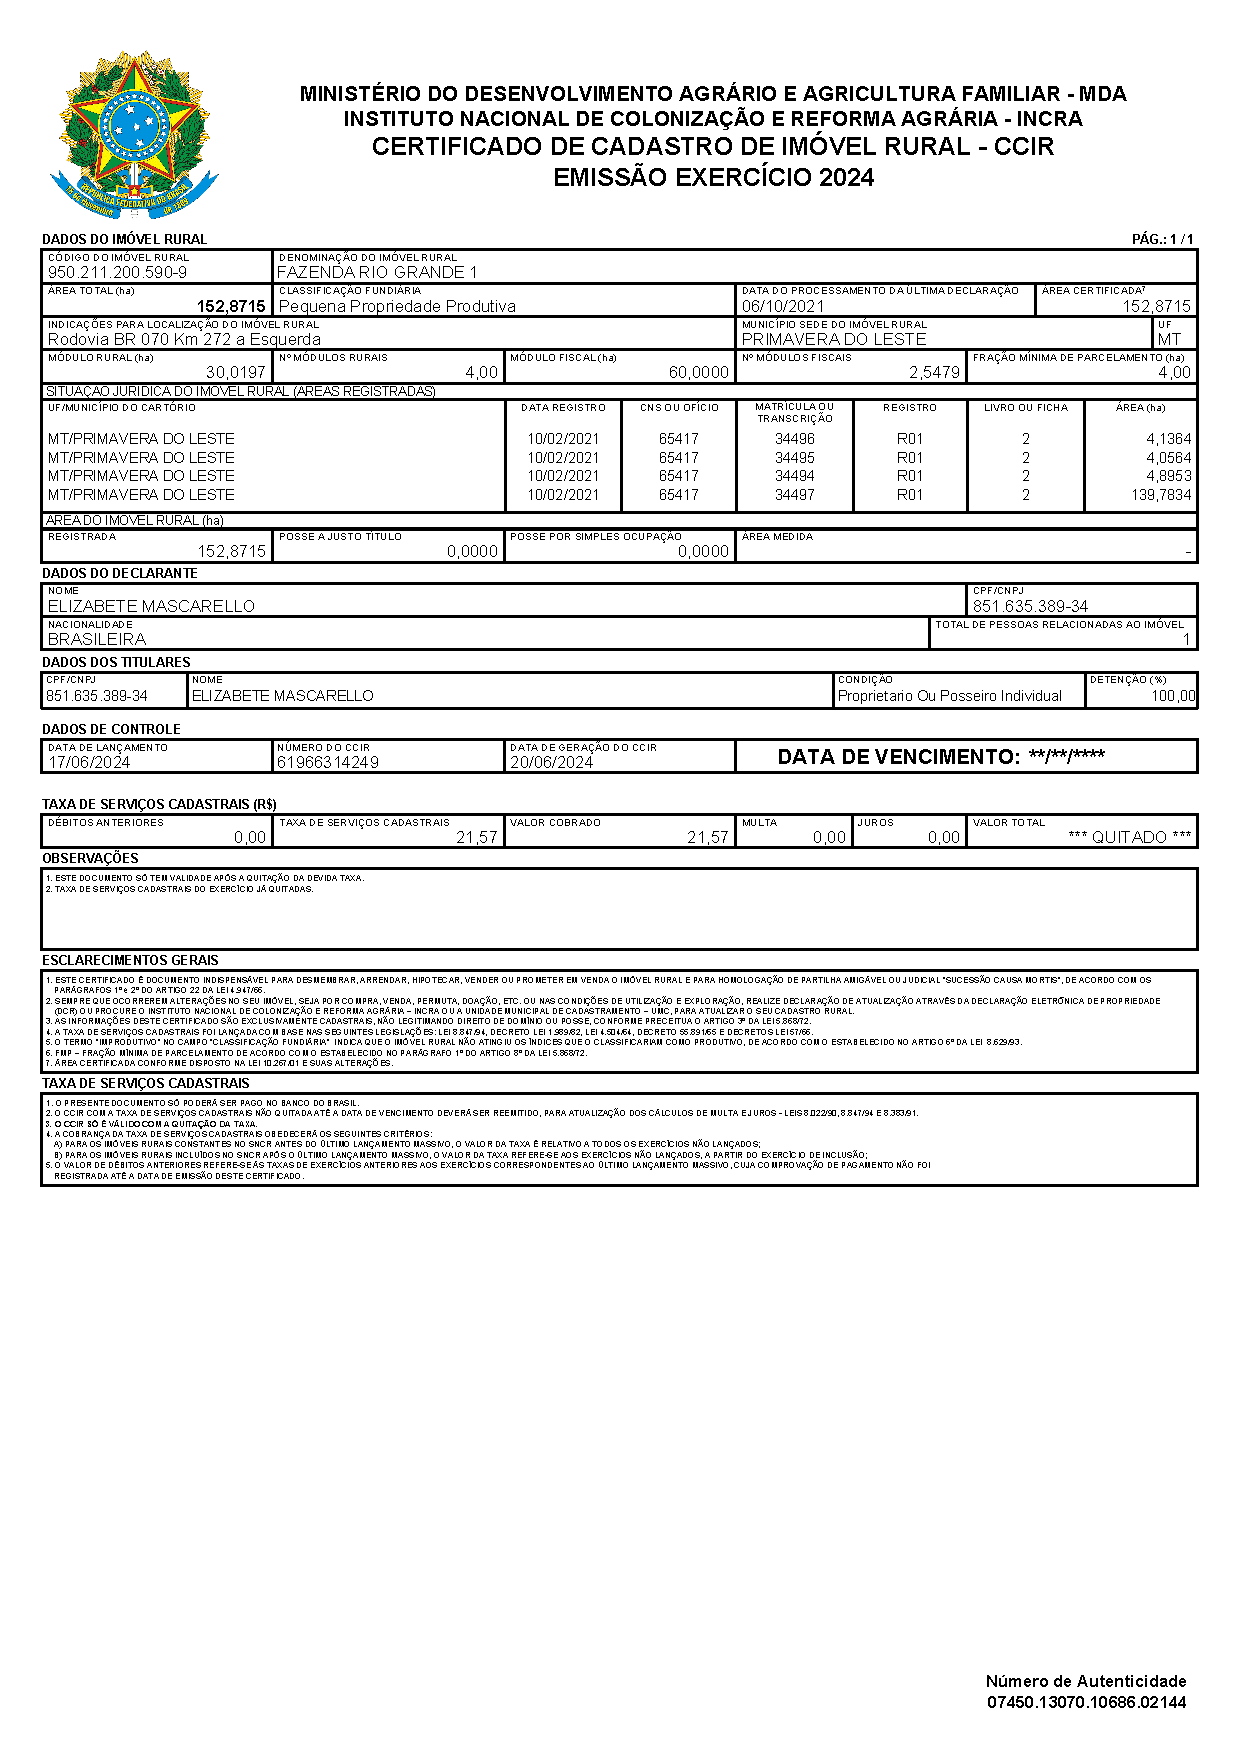
\includepdf[pages={-}]{./refs/CCIR_ELIZABETE.pdf}

\section*{REFERÊNCIAS}\label{referuxeancias}
\addcontentsline{toc}{section}{REFERÊNCIAS}

\phantomsection\label{refs}
\begin{CSLReferences}{0}{0}
\bibitem[\citeproctext]{ref-NBR1465302}
ABNT. \textbf{{NBR} 14653-2: Avaliacao de bens -- parte 2: Imoveis
urbanos}. Rio de Janeiro: Associacao Brasileira de Normas Tecnicas,
2011.

\bibitem[\citeproctext]{ref-NBR1465301}
ABNT. \textbf{{NBR} 14653-1: Avaliacao de bens -- parte 1: Procedimentos
gerais}. Rio de Janeiro: Associacao Brasileira de Normas Tecnicas, 2019.

\end{CSLReferences}

\end{document}
